\chapter{DESENVOLVIMENTO E RESULTADOS}\label{cap:desenvolvimento}

Este capítulo apresenta a implementação do sistema de comunicação digital proposto, detalhando cada etapa do processo, desde a geração dos bits até a recuperação do datagrama no receptor. A seguir, são descritas as principais componentes do sistema, incluindo a cadeia de transmissão, o canal de comunicação com ruído adicionado, a detecção de portadora e a cadeia de recepção.

\section{CADEIA DE TRANSMISSÃO}\label{sec:transmissao}

teste

\subsection{Sequência de transmissão}\label{sec:geracao_bits}

\begin{figure}[H]
	\centering
	\caption{Streambits do datagrama ARGOS-3}\label{fig:datagrama_time}
	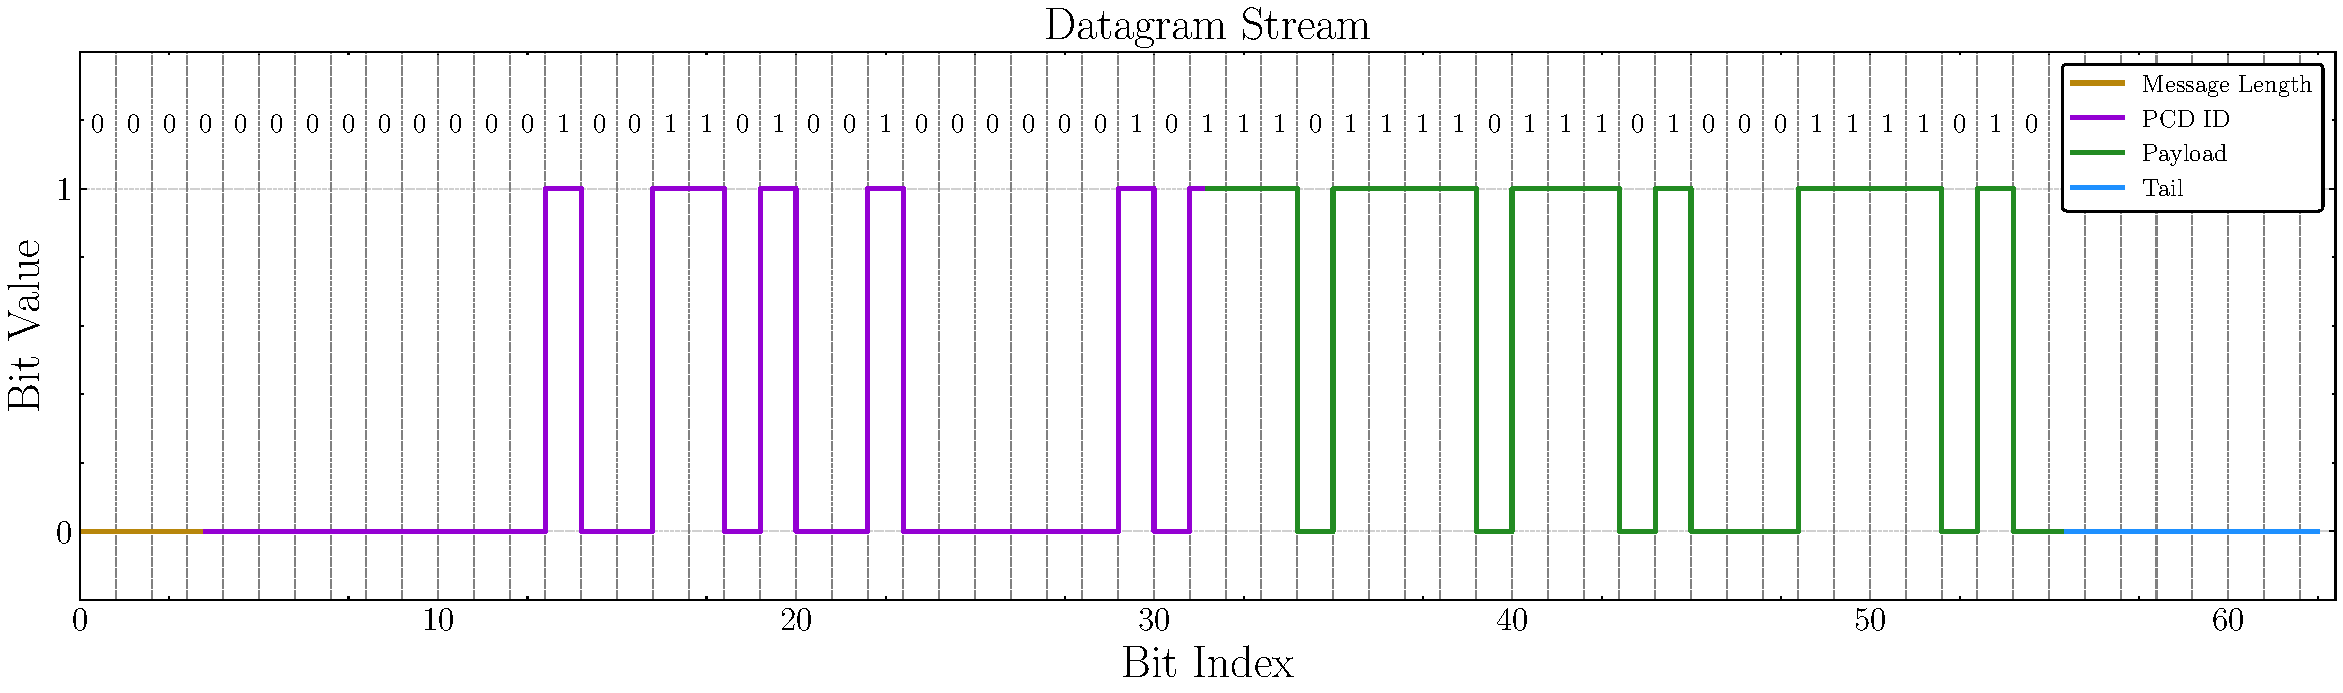
\includegraphics[width=\linewidth]{assets/cap3/transmitter_datagram_time.pdf}
\end{figure}

\begin{figure}[H]
	\centering
	\caption{Multiplexação com preâmbulo}\label{fig:mux_time}
	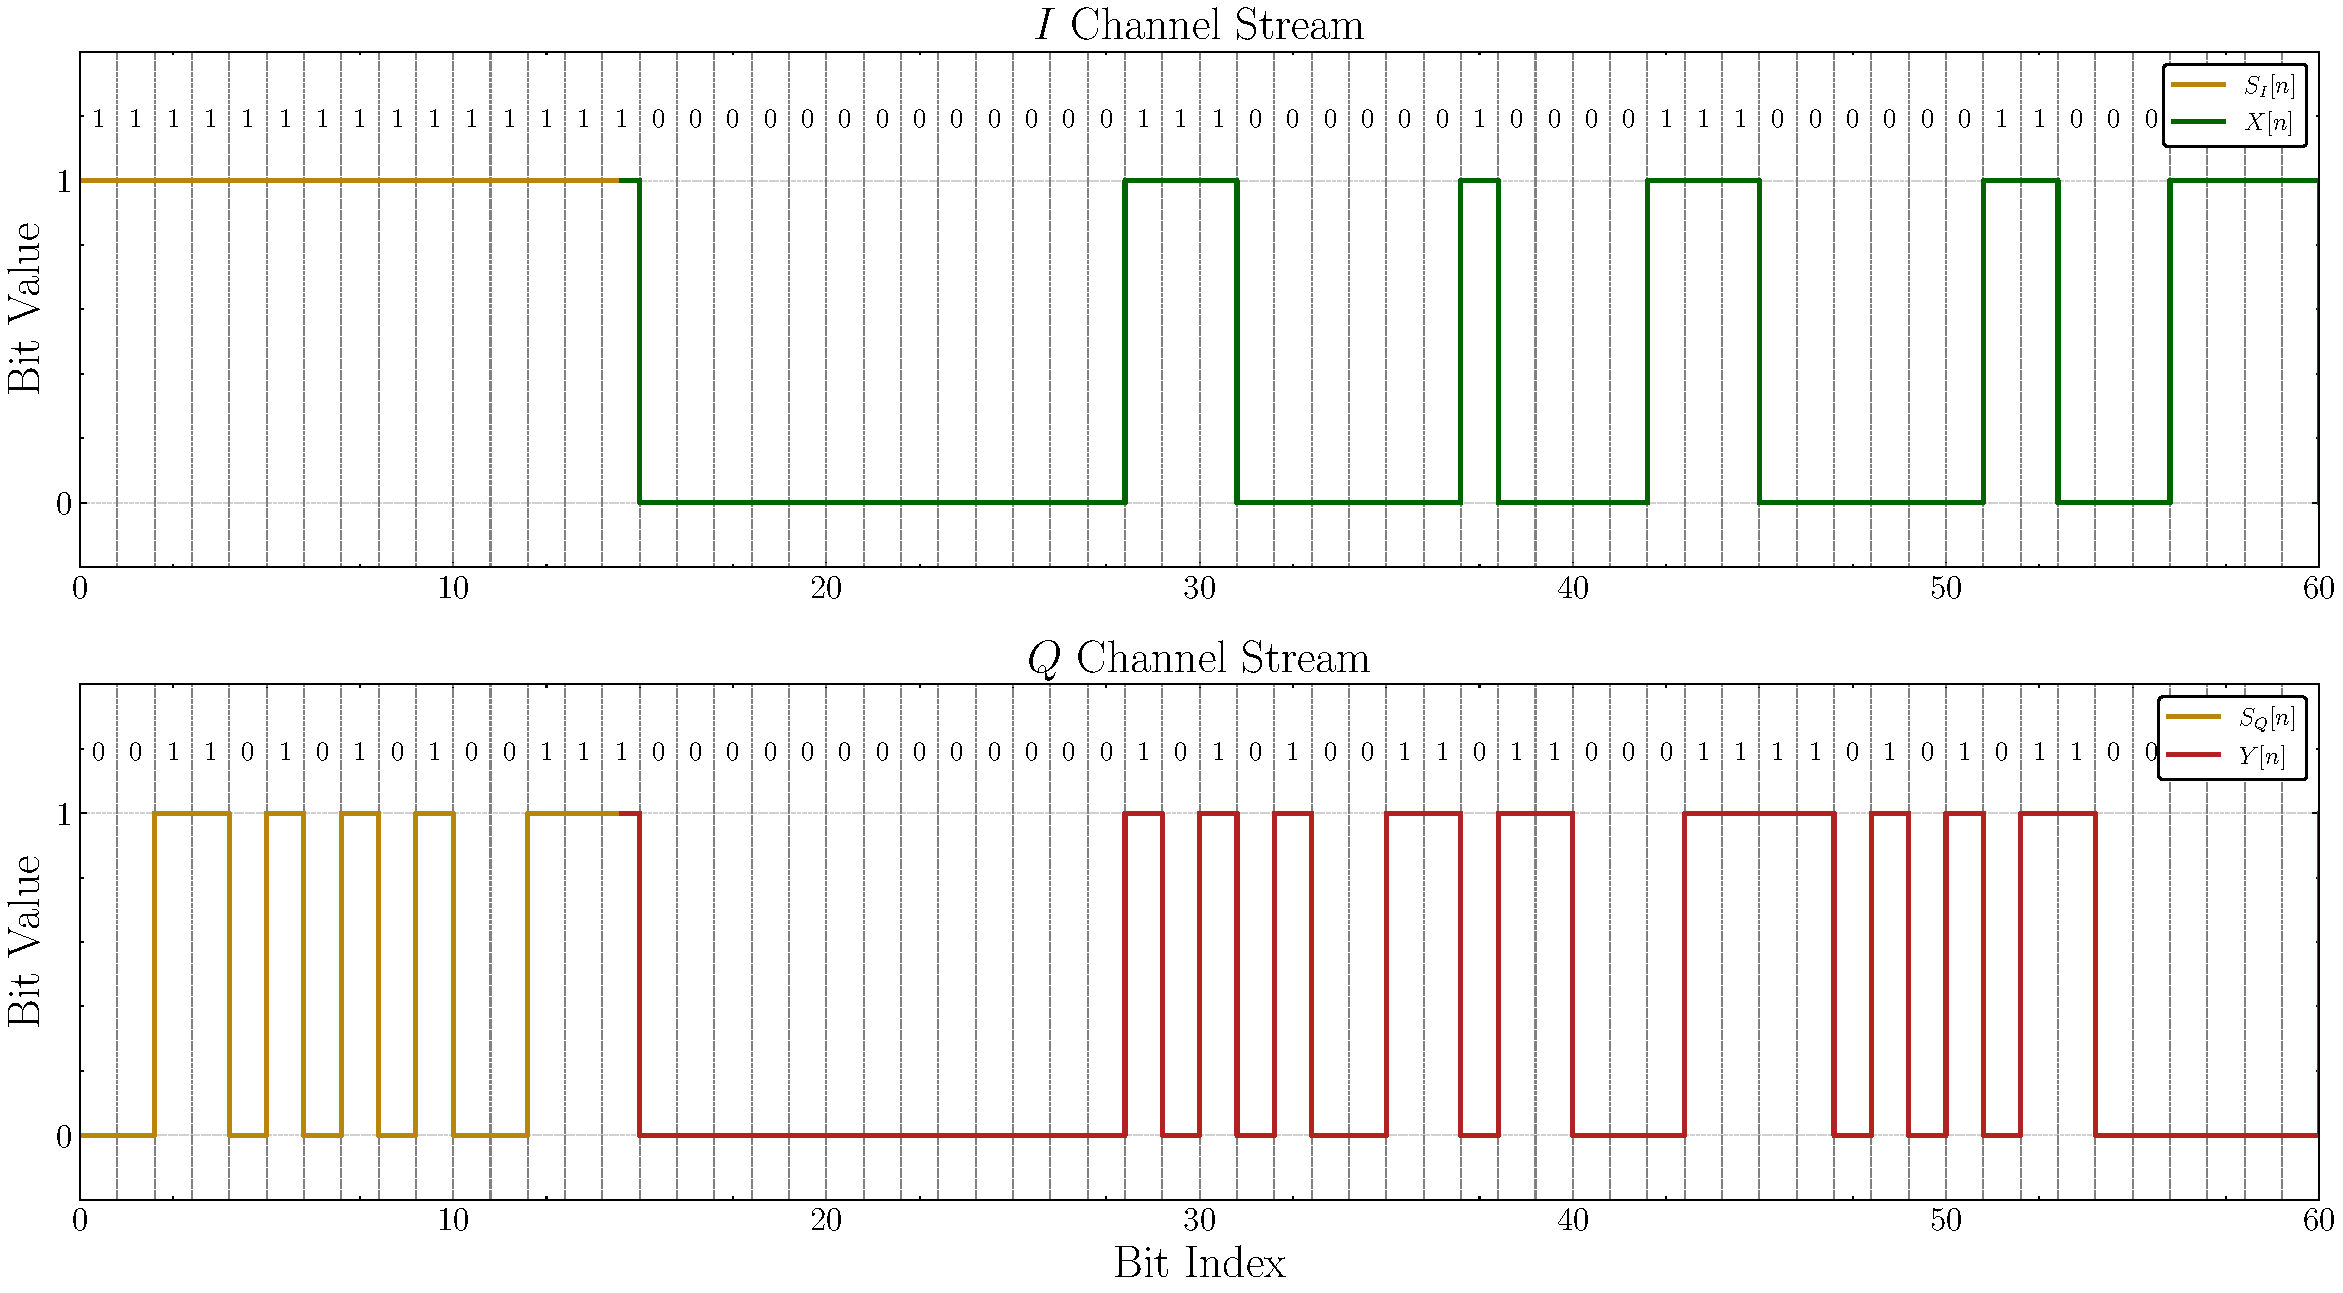
\includegraphics[width=\linewidth]{assets/cap3/transmitter_mux_time.pdf}
\end{figure}


\begin{figure}[H]
	\centering
	\caption{Codificação de linha}\label{fig:encoder_time}
	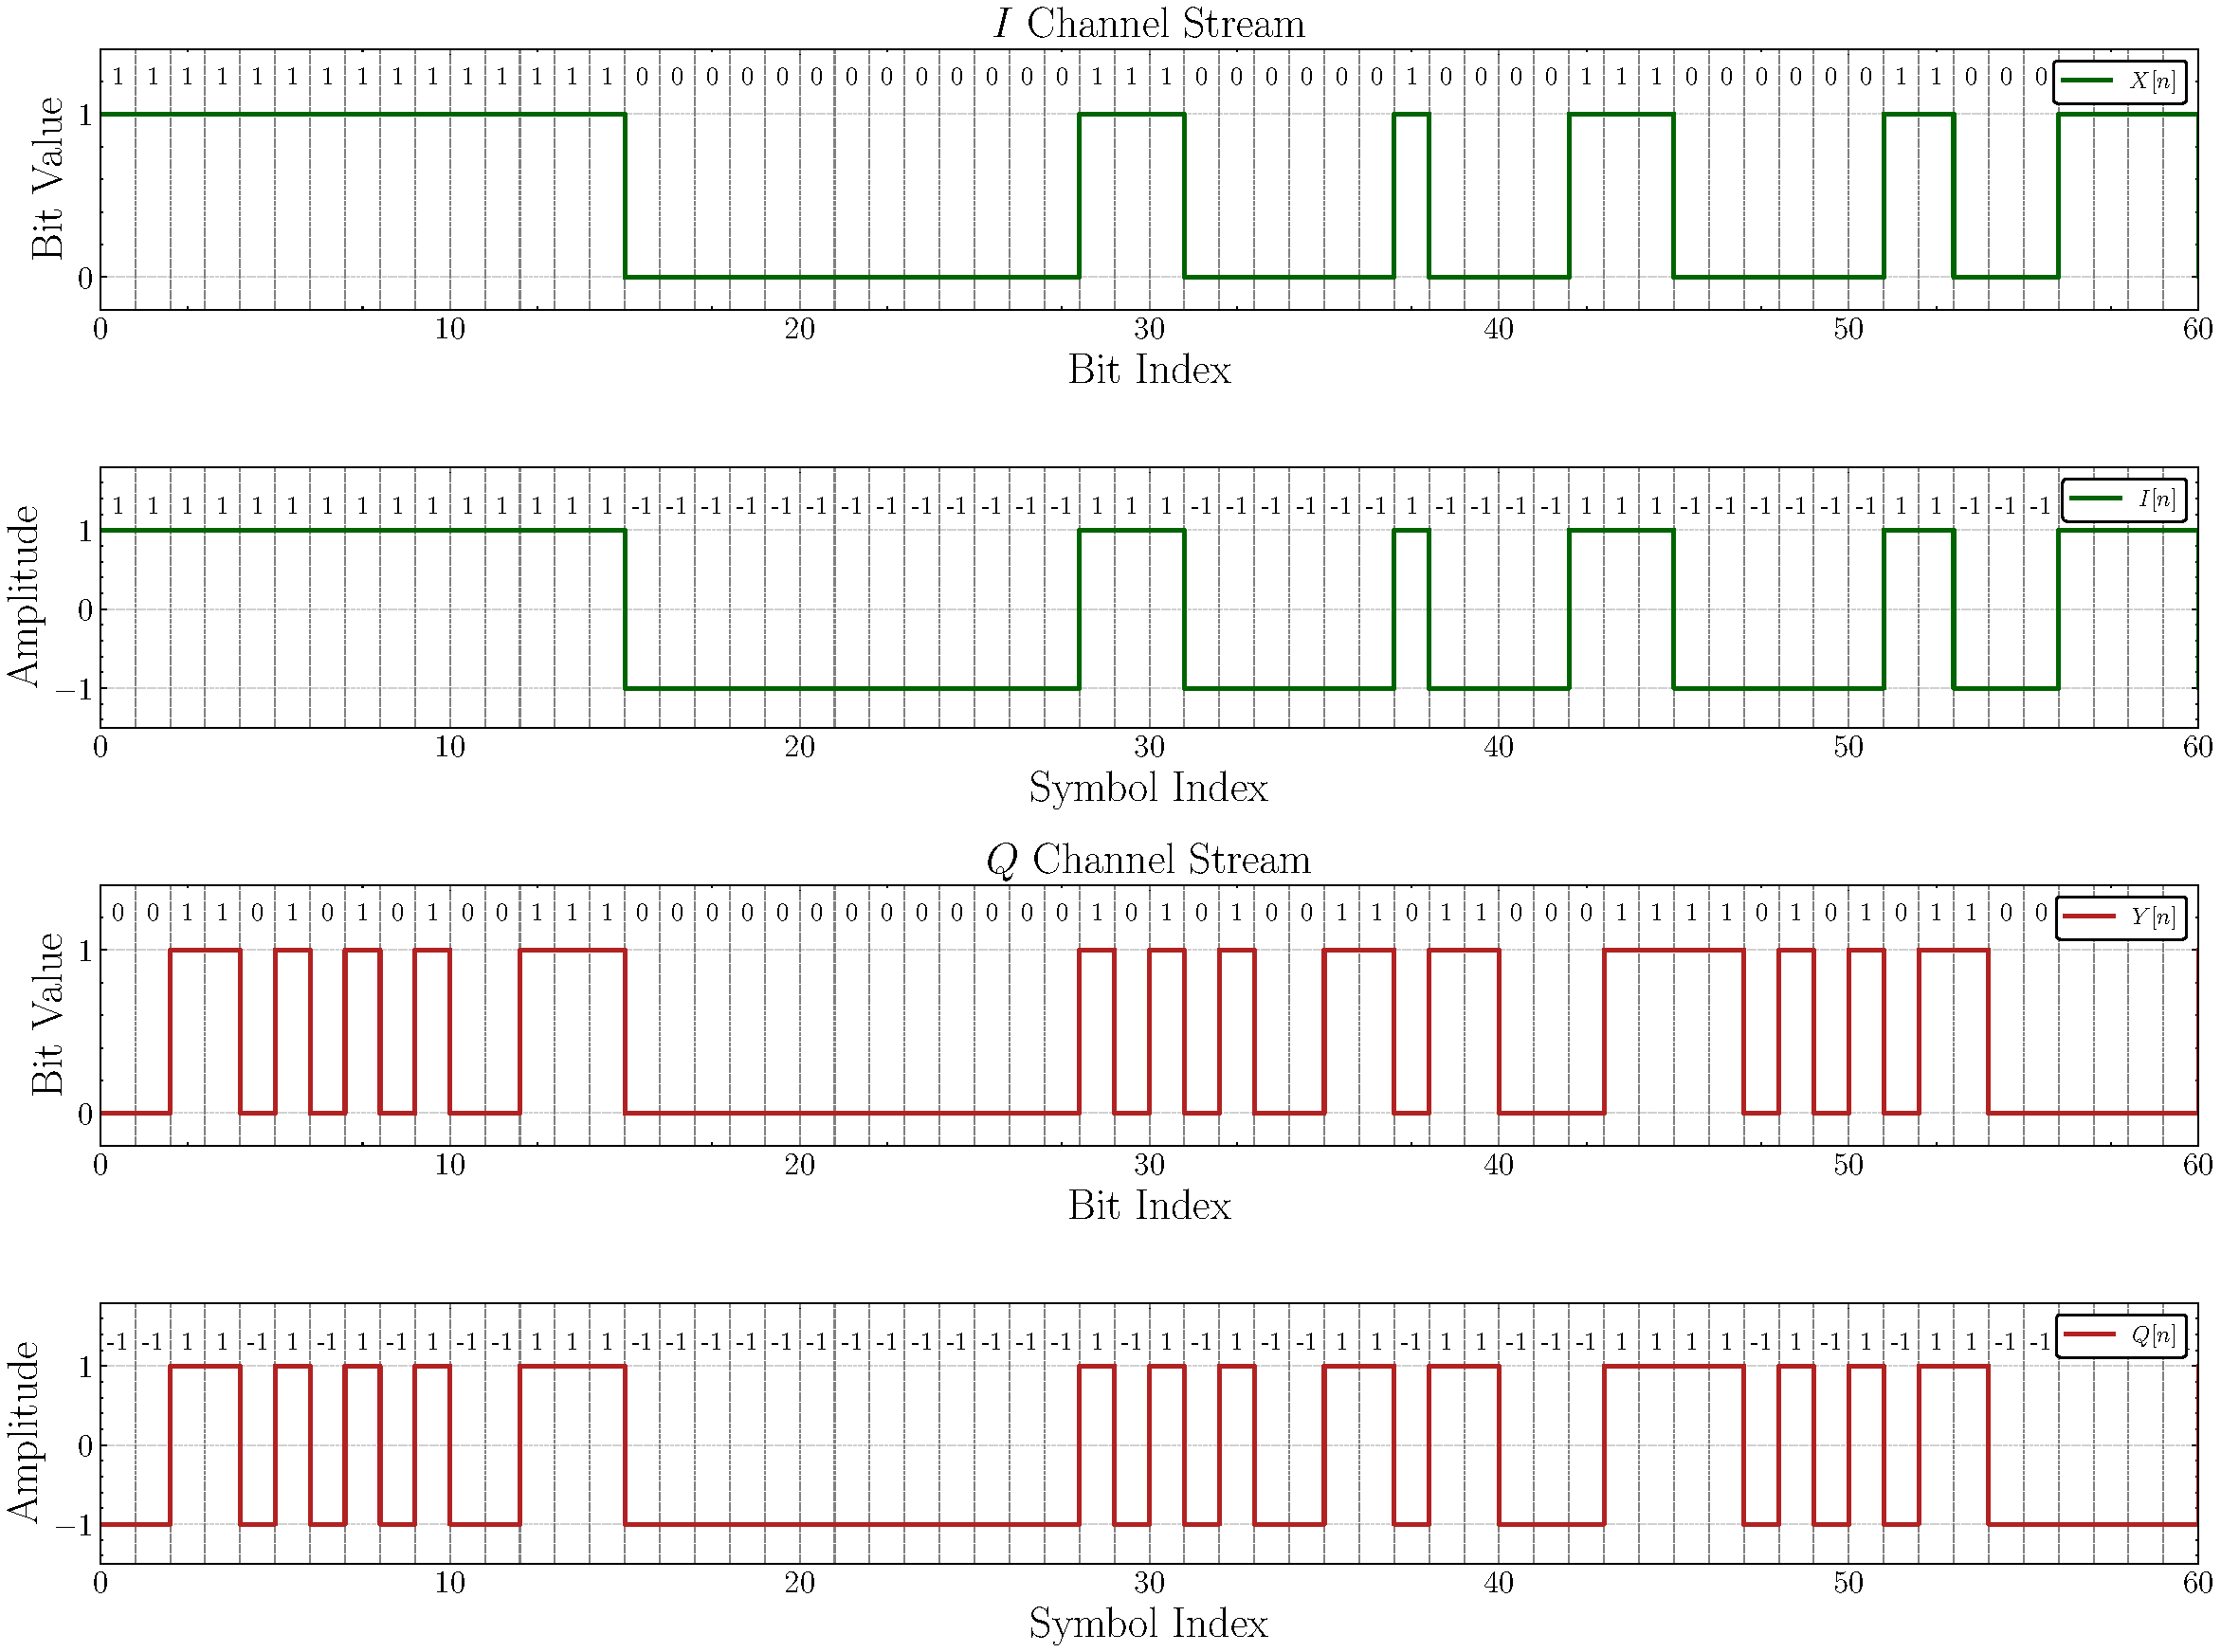
\includegraphics[width=\linewidth]{assets/cap3/transmitter_encoder_time.pdf}
\end{figure}

\subsection{Modulação de pulso RRC e Manchester}



\subsubsection{Pulso RRC e Manchester}

\begin{figure}[H]
	\centering
	\caption{Resposta ao impulso - Pulso RRC}\label{fig:impulse_response_rrc}
	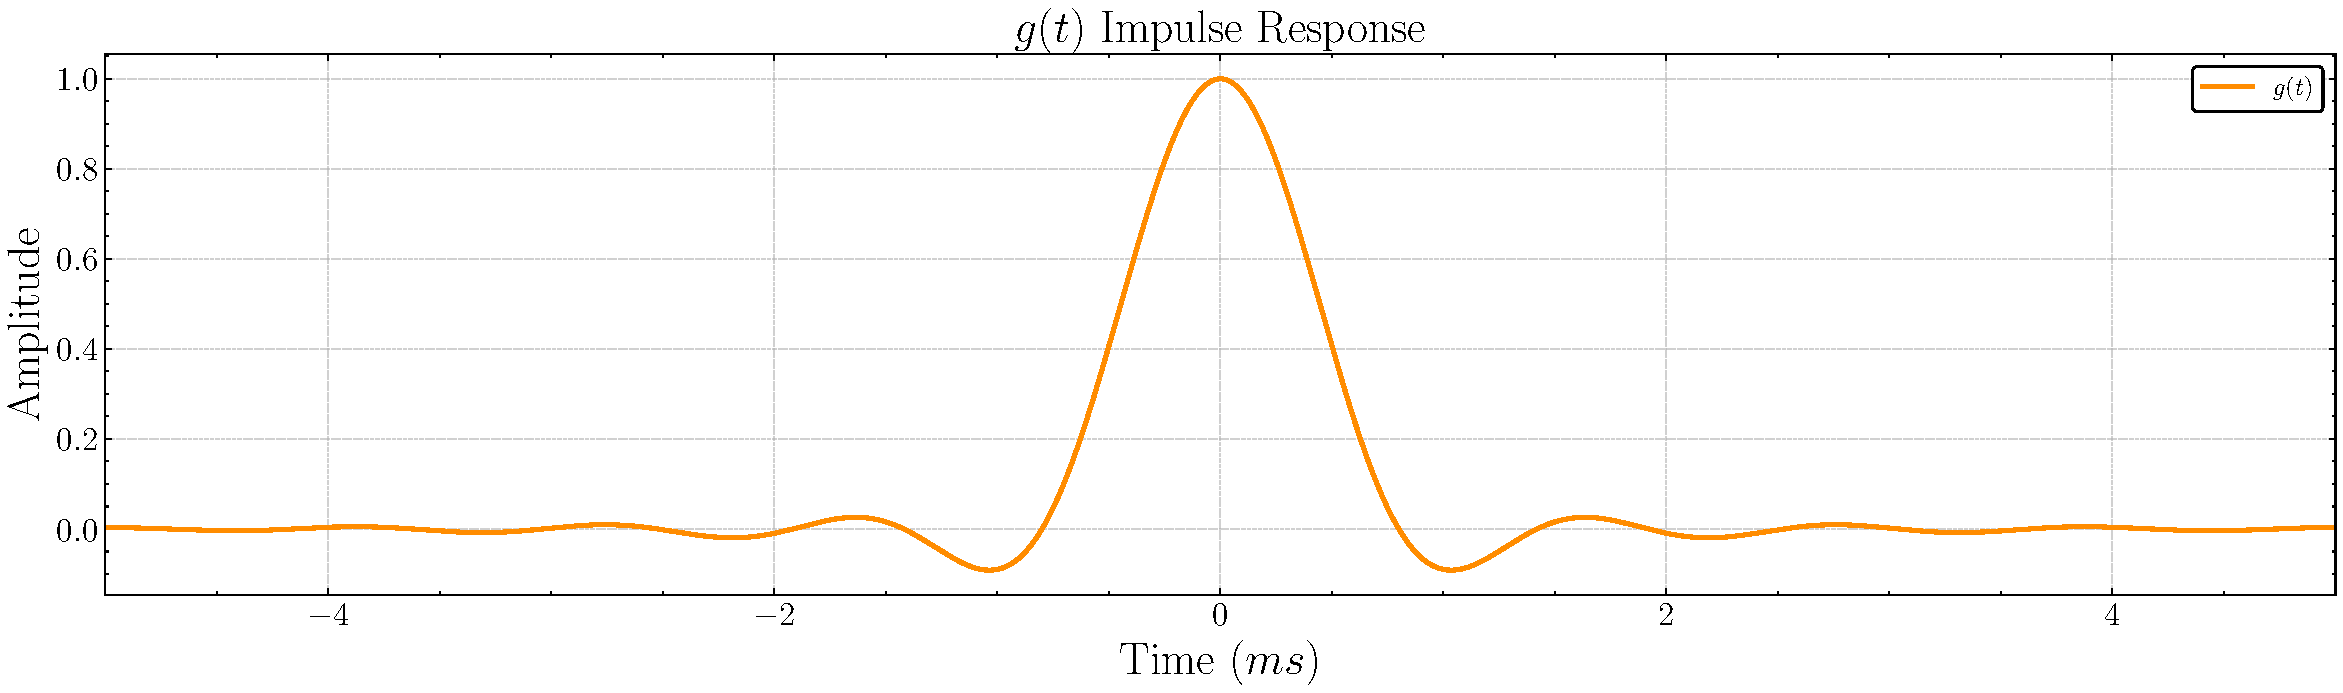
\includegraphics[width=\linewidth]{assets/cap3/example_formatter_impulse.pdf}
\end{figure}

\begin{figure}[H]
	\centering
	\caption{Resposta ao impulso - Pulso Manchester}\label{fig:impulse_response_man}
	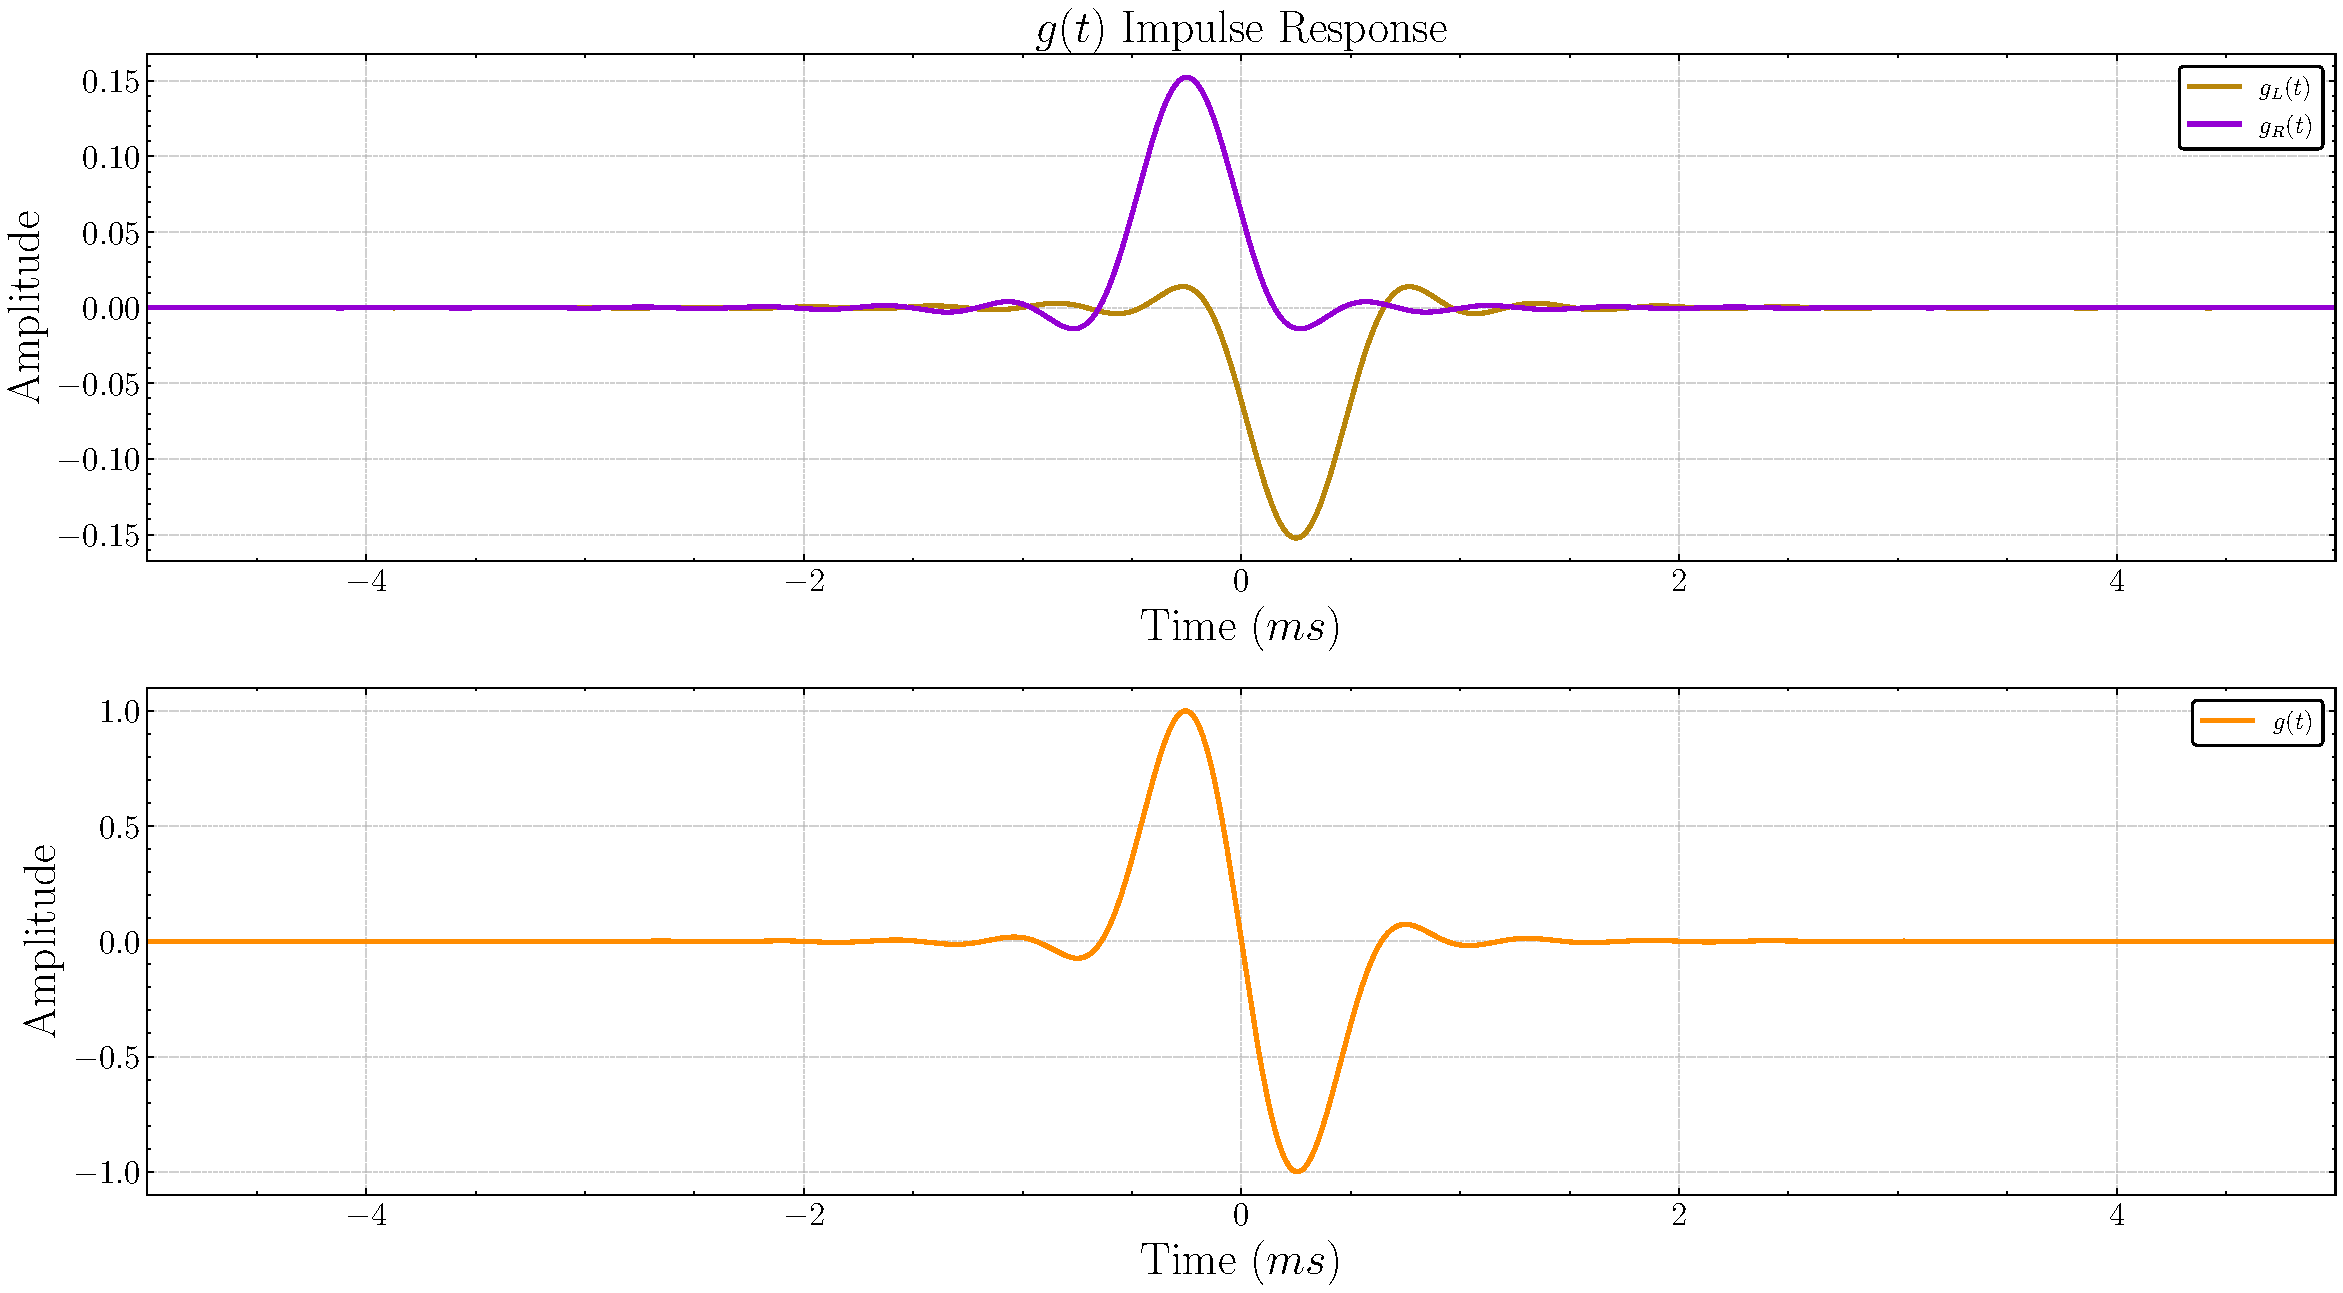
\includegraphics[width=\linewidth]{assets/cap3/example_formatter_impulse_man.pdf}
\end{figure}


\subsubsection{Modulação de pulso dos canais I e Q}


\begin{figure}[H]
	\centering
	\caption{Modulação de pulso dos canais I e Q}\label{fig:transmitter_formatter_time}
	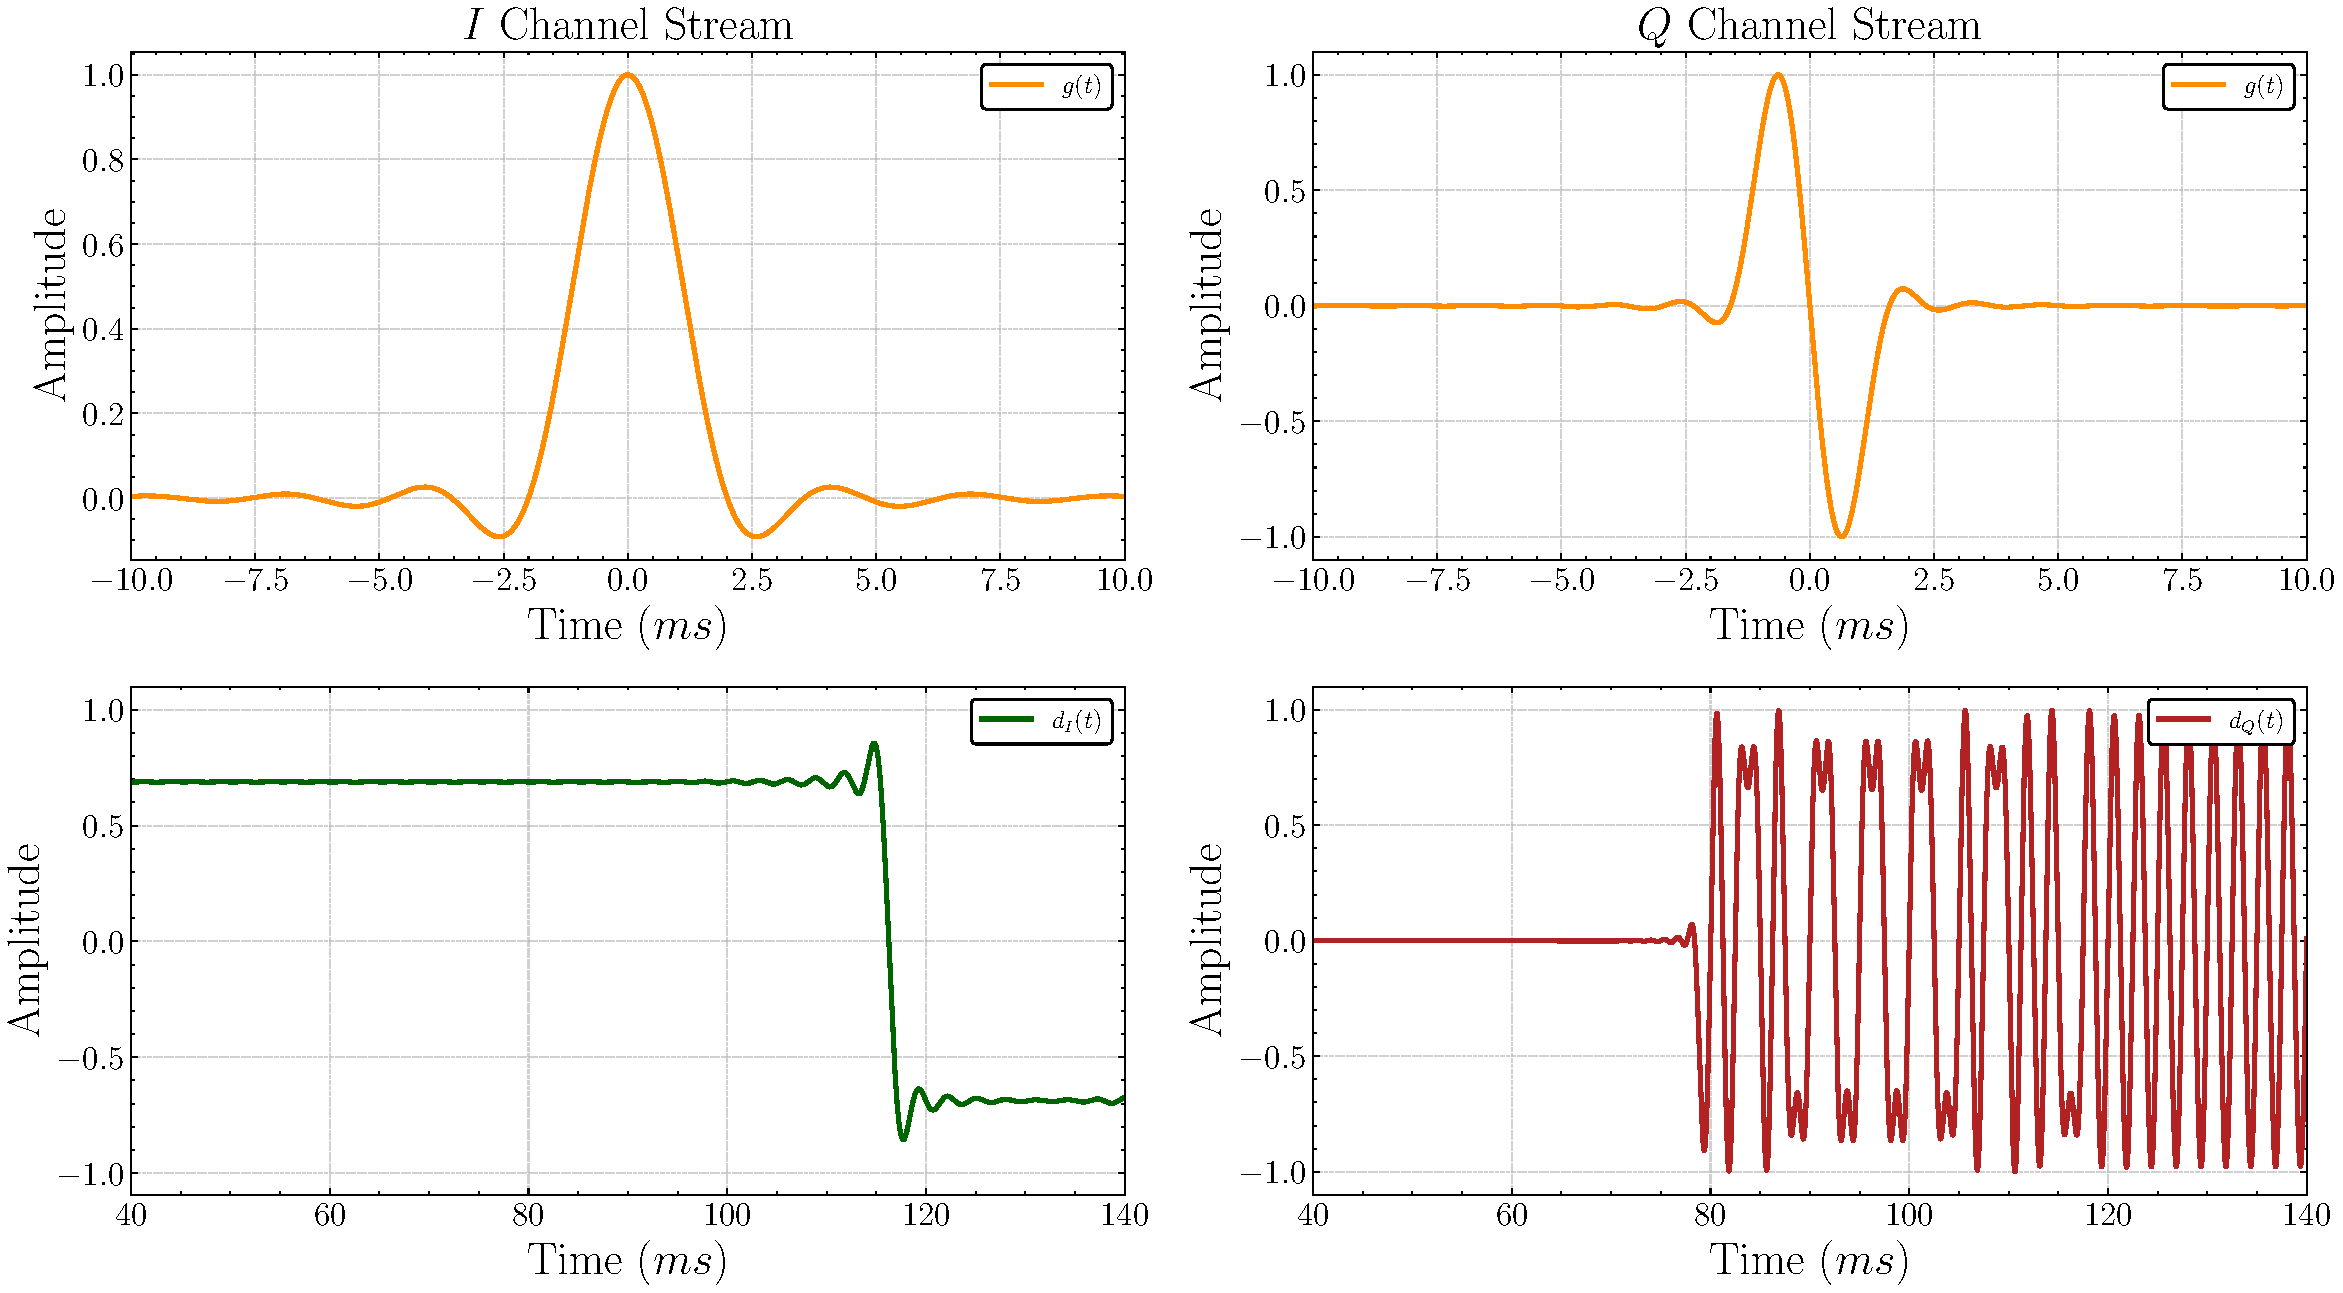
\includegraphics[width=\linewidth]{assets/cap3/transmitter_formatter_time.pdf}
\end{figure}


\subsection{Modulação em fase em quadratura (QPSK)}\label{sec:qpsk}

\begin{figure}[H]
	\centering
	\caption{Modulação em banda passante canais $I$ e $Q$}\label{fig:transmitter_modulator_time}
	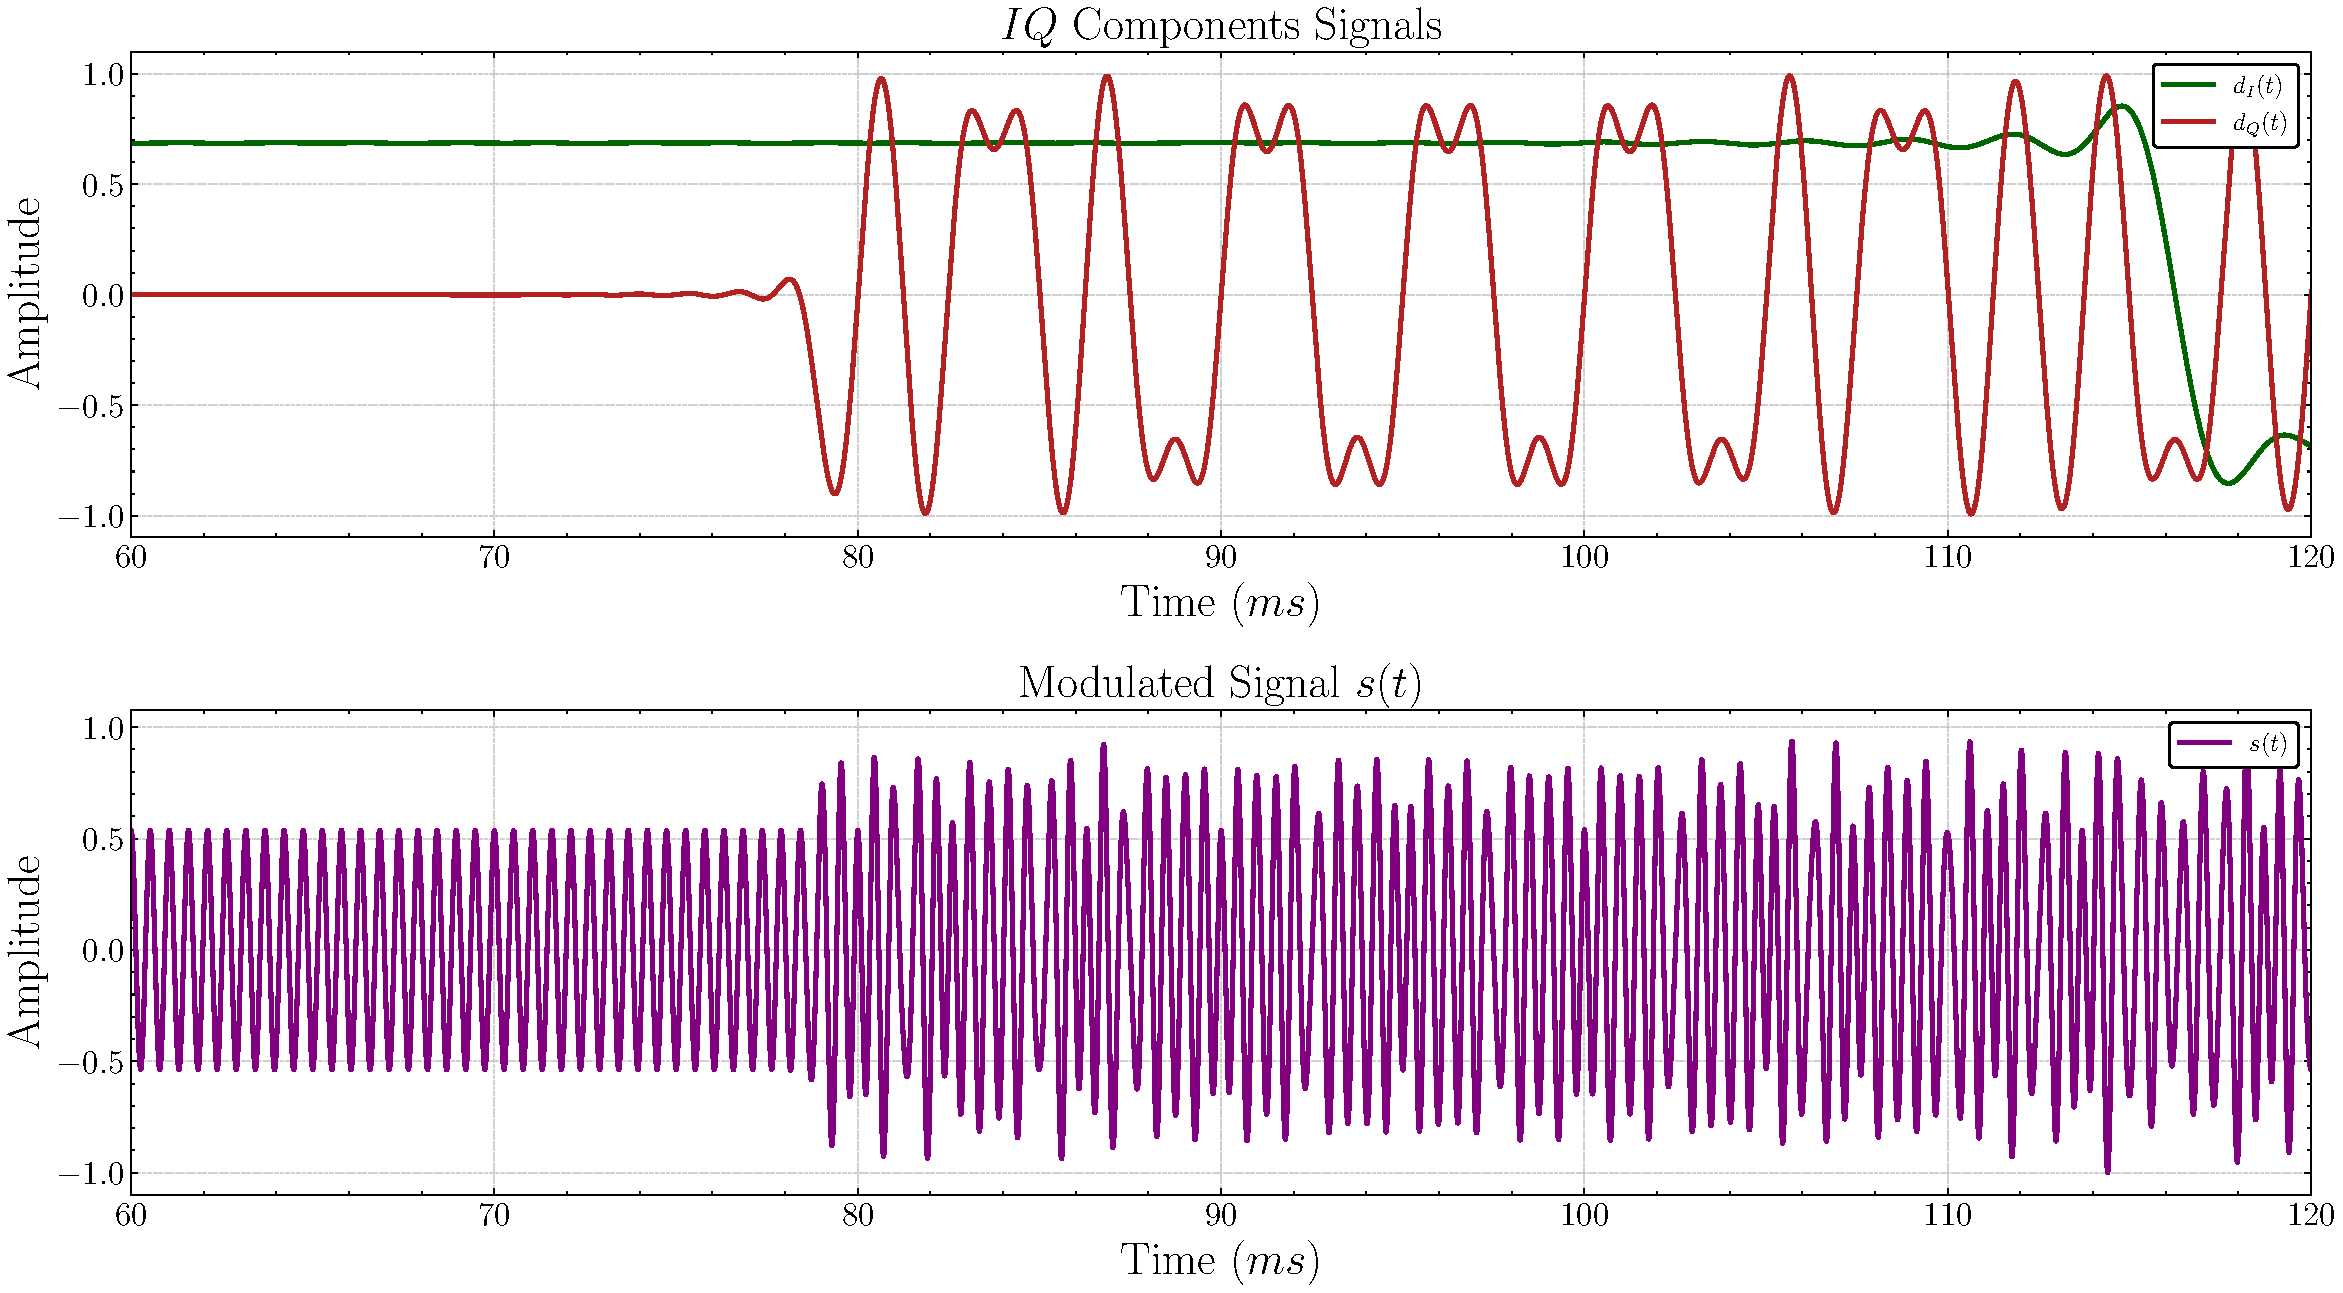
\includegraphics[width=\linewidth]{assets/cap3/transmitter_modulator_time.pdf}
\end{figure}


\begin{figure}[H]
	\centering
	\caption{Fase e Constelação do sinal modulado $s(t)$}\label{fig:transmitter_modulator_constellation}
	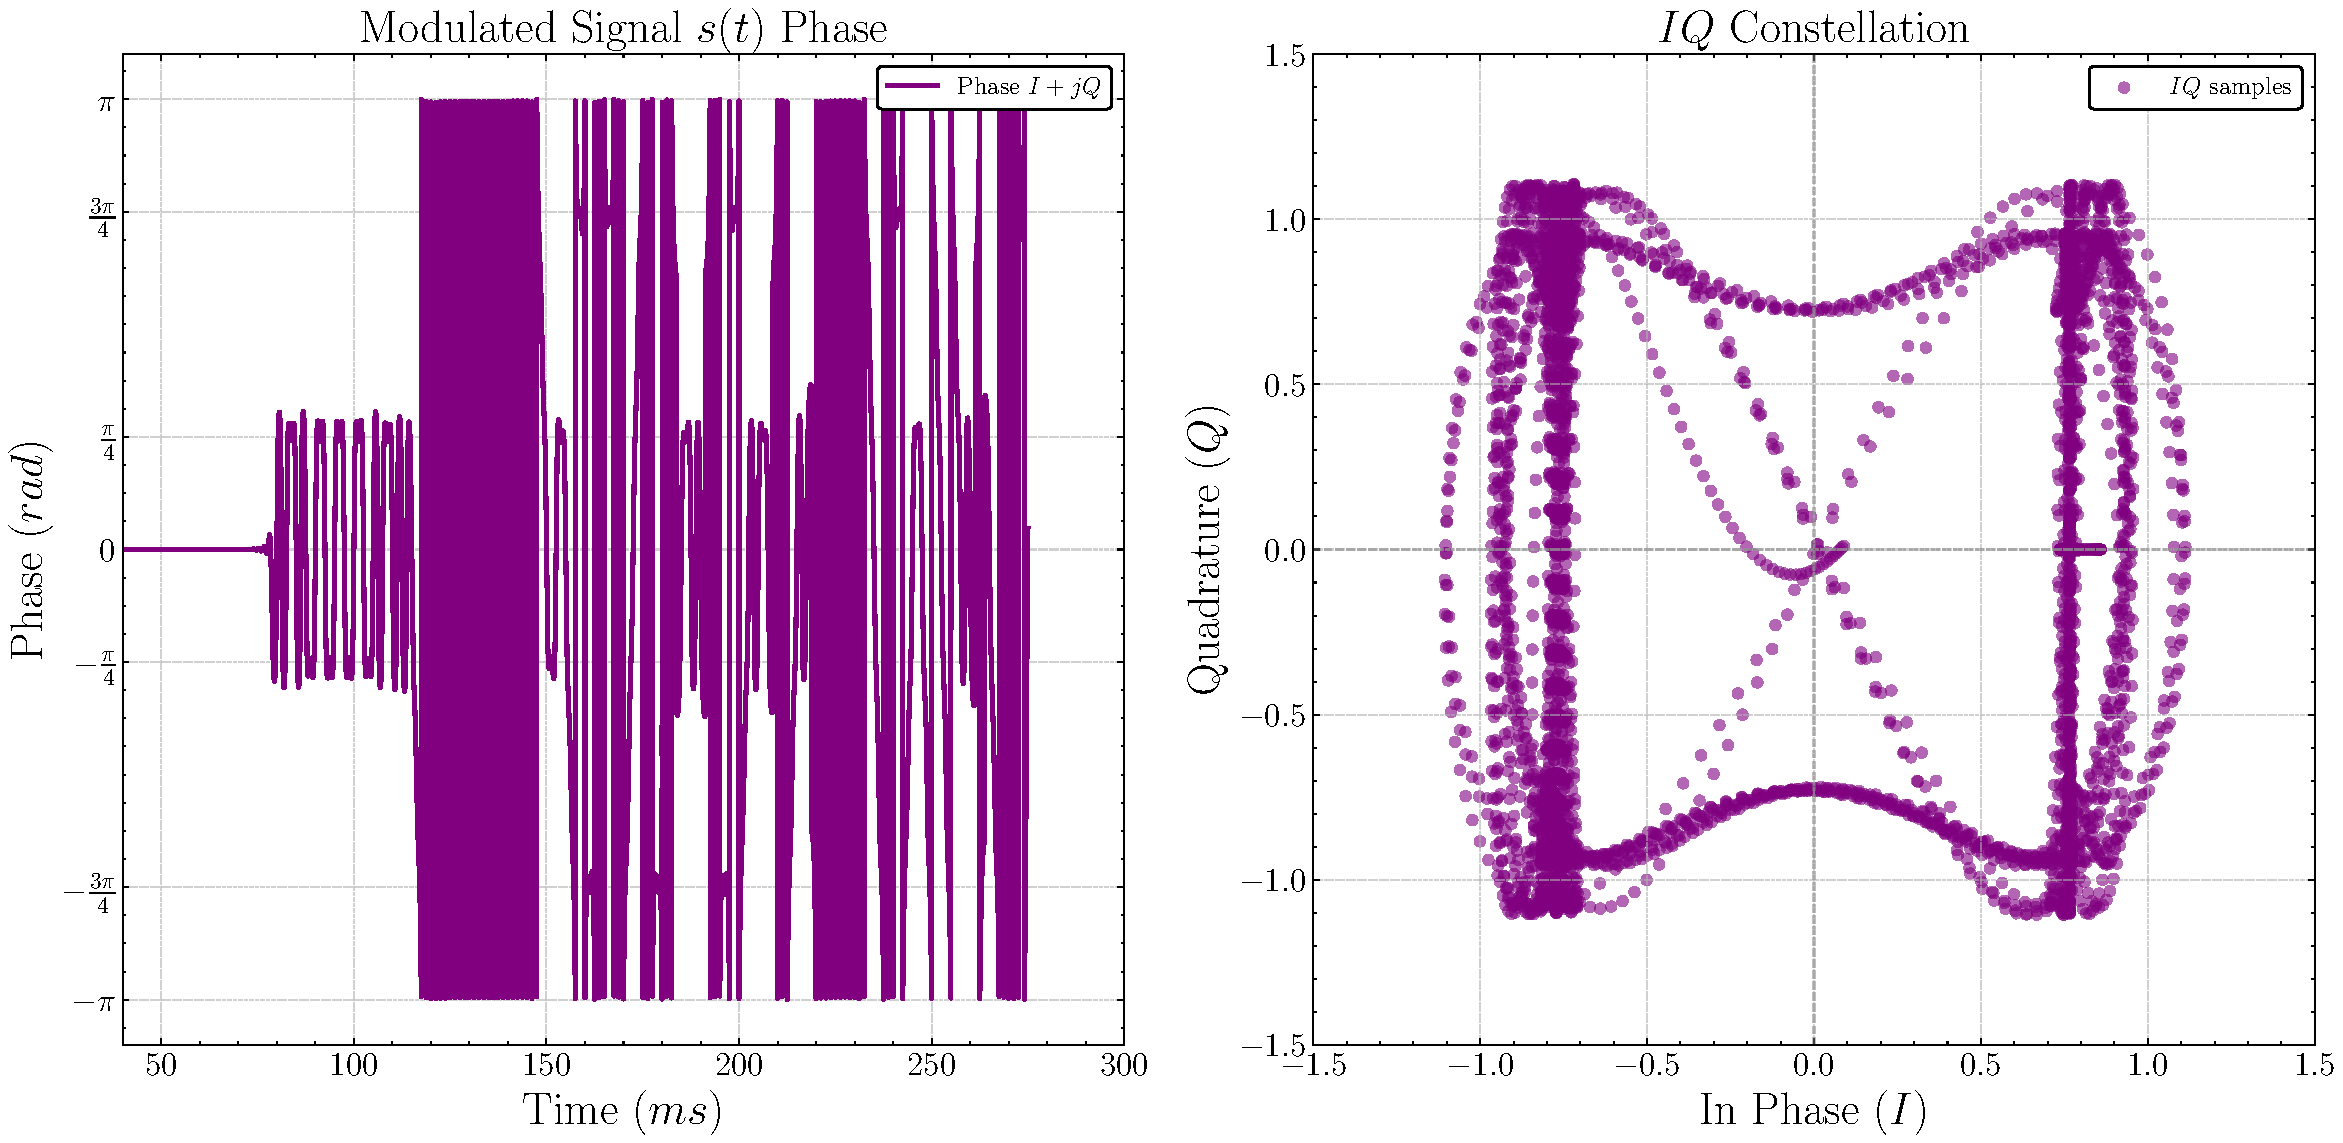
\includegraphics[width=\linewidth]{assets/cap3/transmitter_modulator_constellation.pdf}
\end{figure}


\subsubsection{Adição de portadora pura}

\begin{figure}[H]
	\centering
	\caption{Comparação de portadora pura e sinal modulado}\label{fig:transmitter_modulator_portadora}
	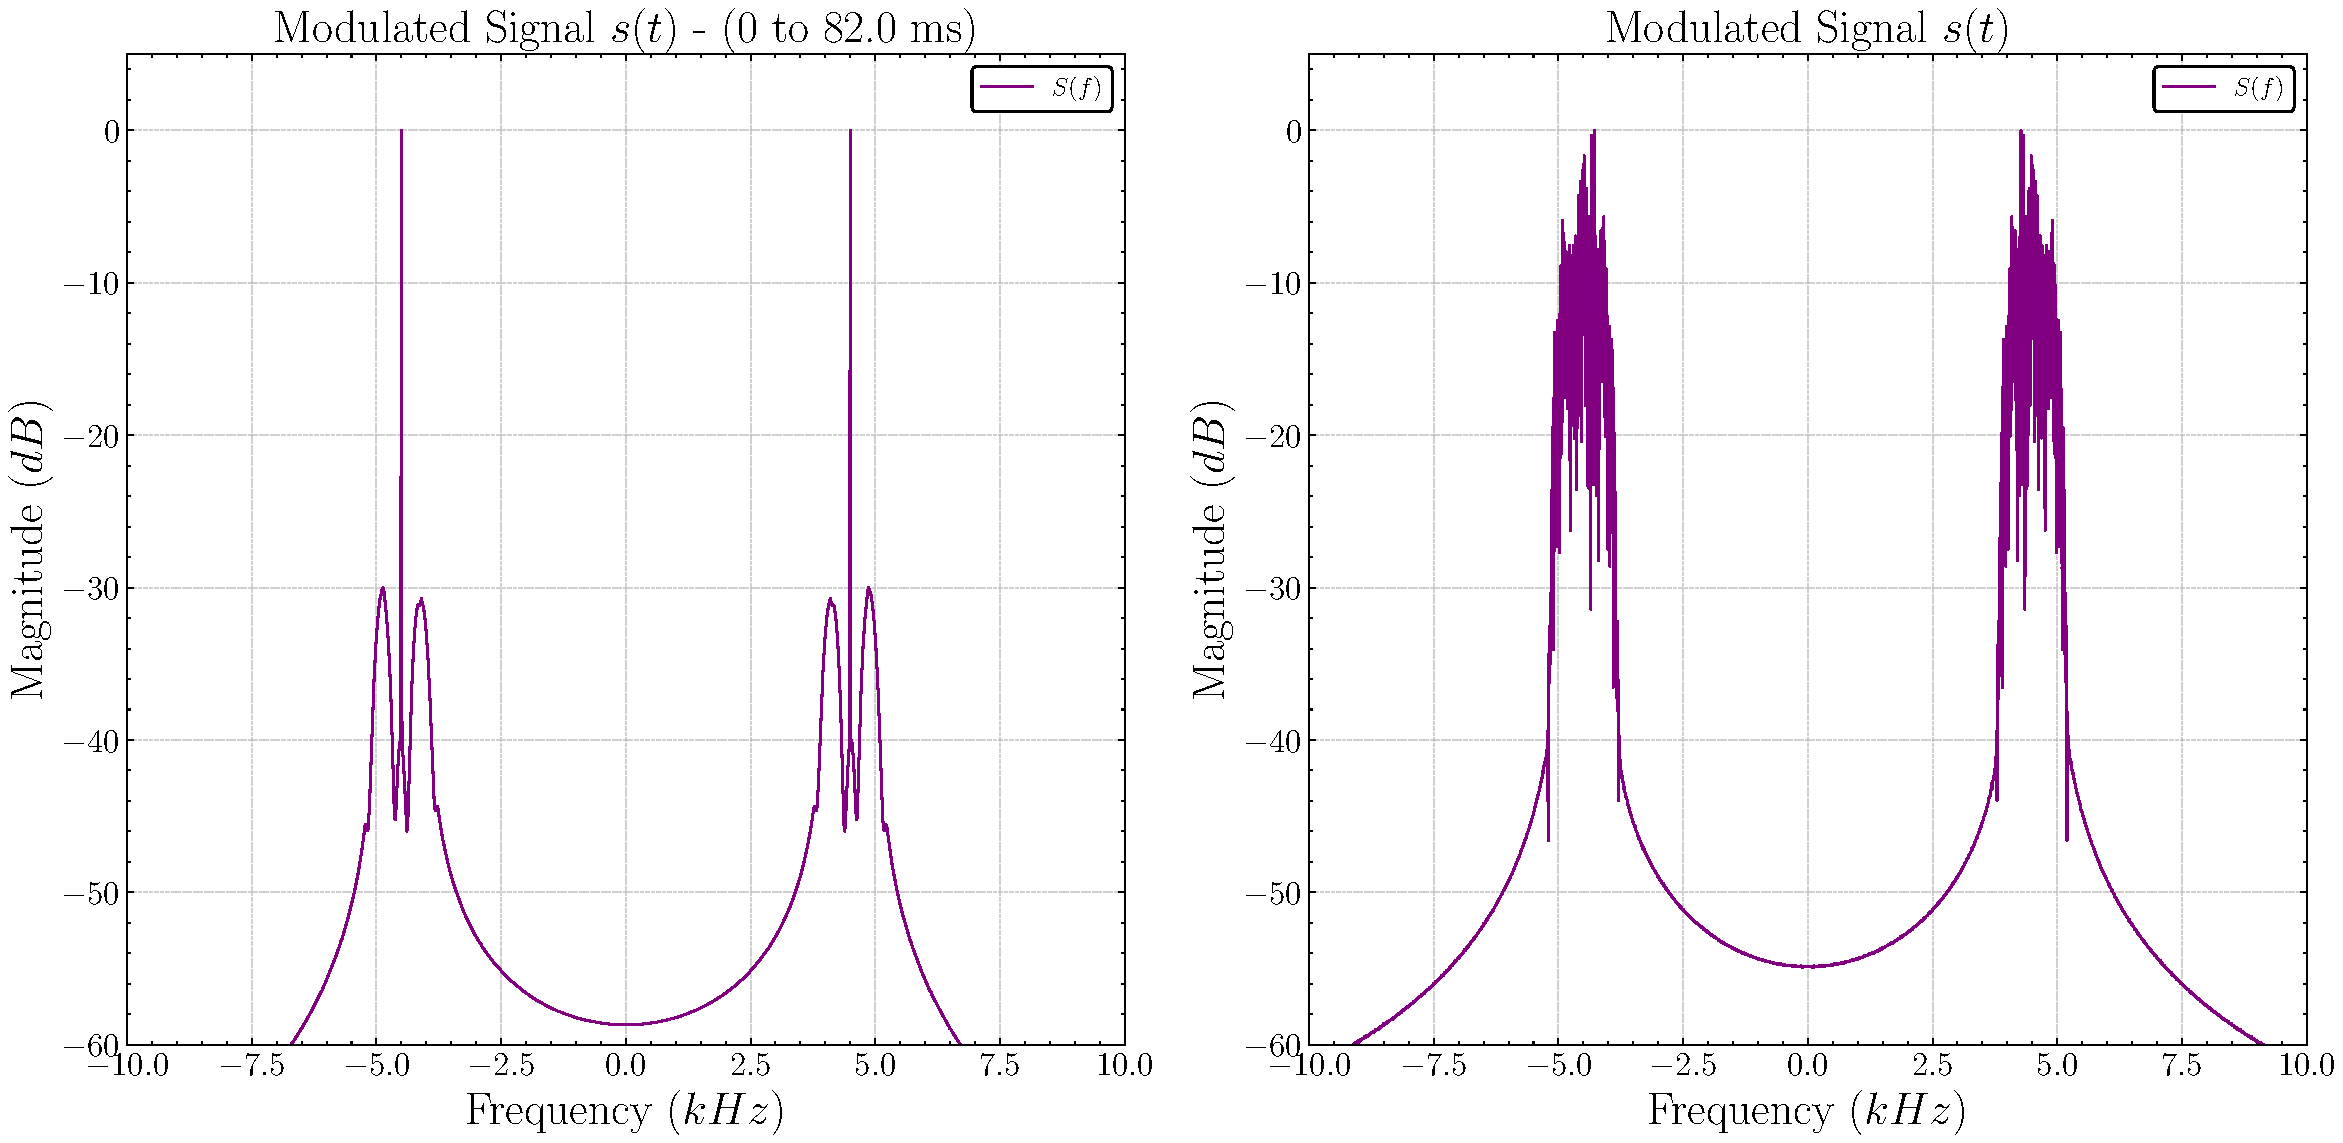
\includegraphics[width=\linewidth]{assets/cap3/transmitter_modulator_portadora.pdf}
\end{figure}


\section{CANAL E ADIÇÃO DE RUÍDO}\label{sec:canal}

\subsection{Modelo de canal}\label{sec:modelo_canal}

\begin{figure}[H]
	\centering
	\caption{Adição de multiplas transmissões no canal}\label{fig:channel_time}
	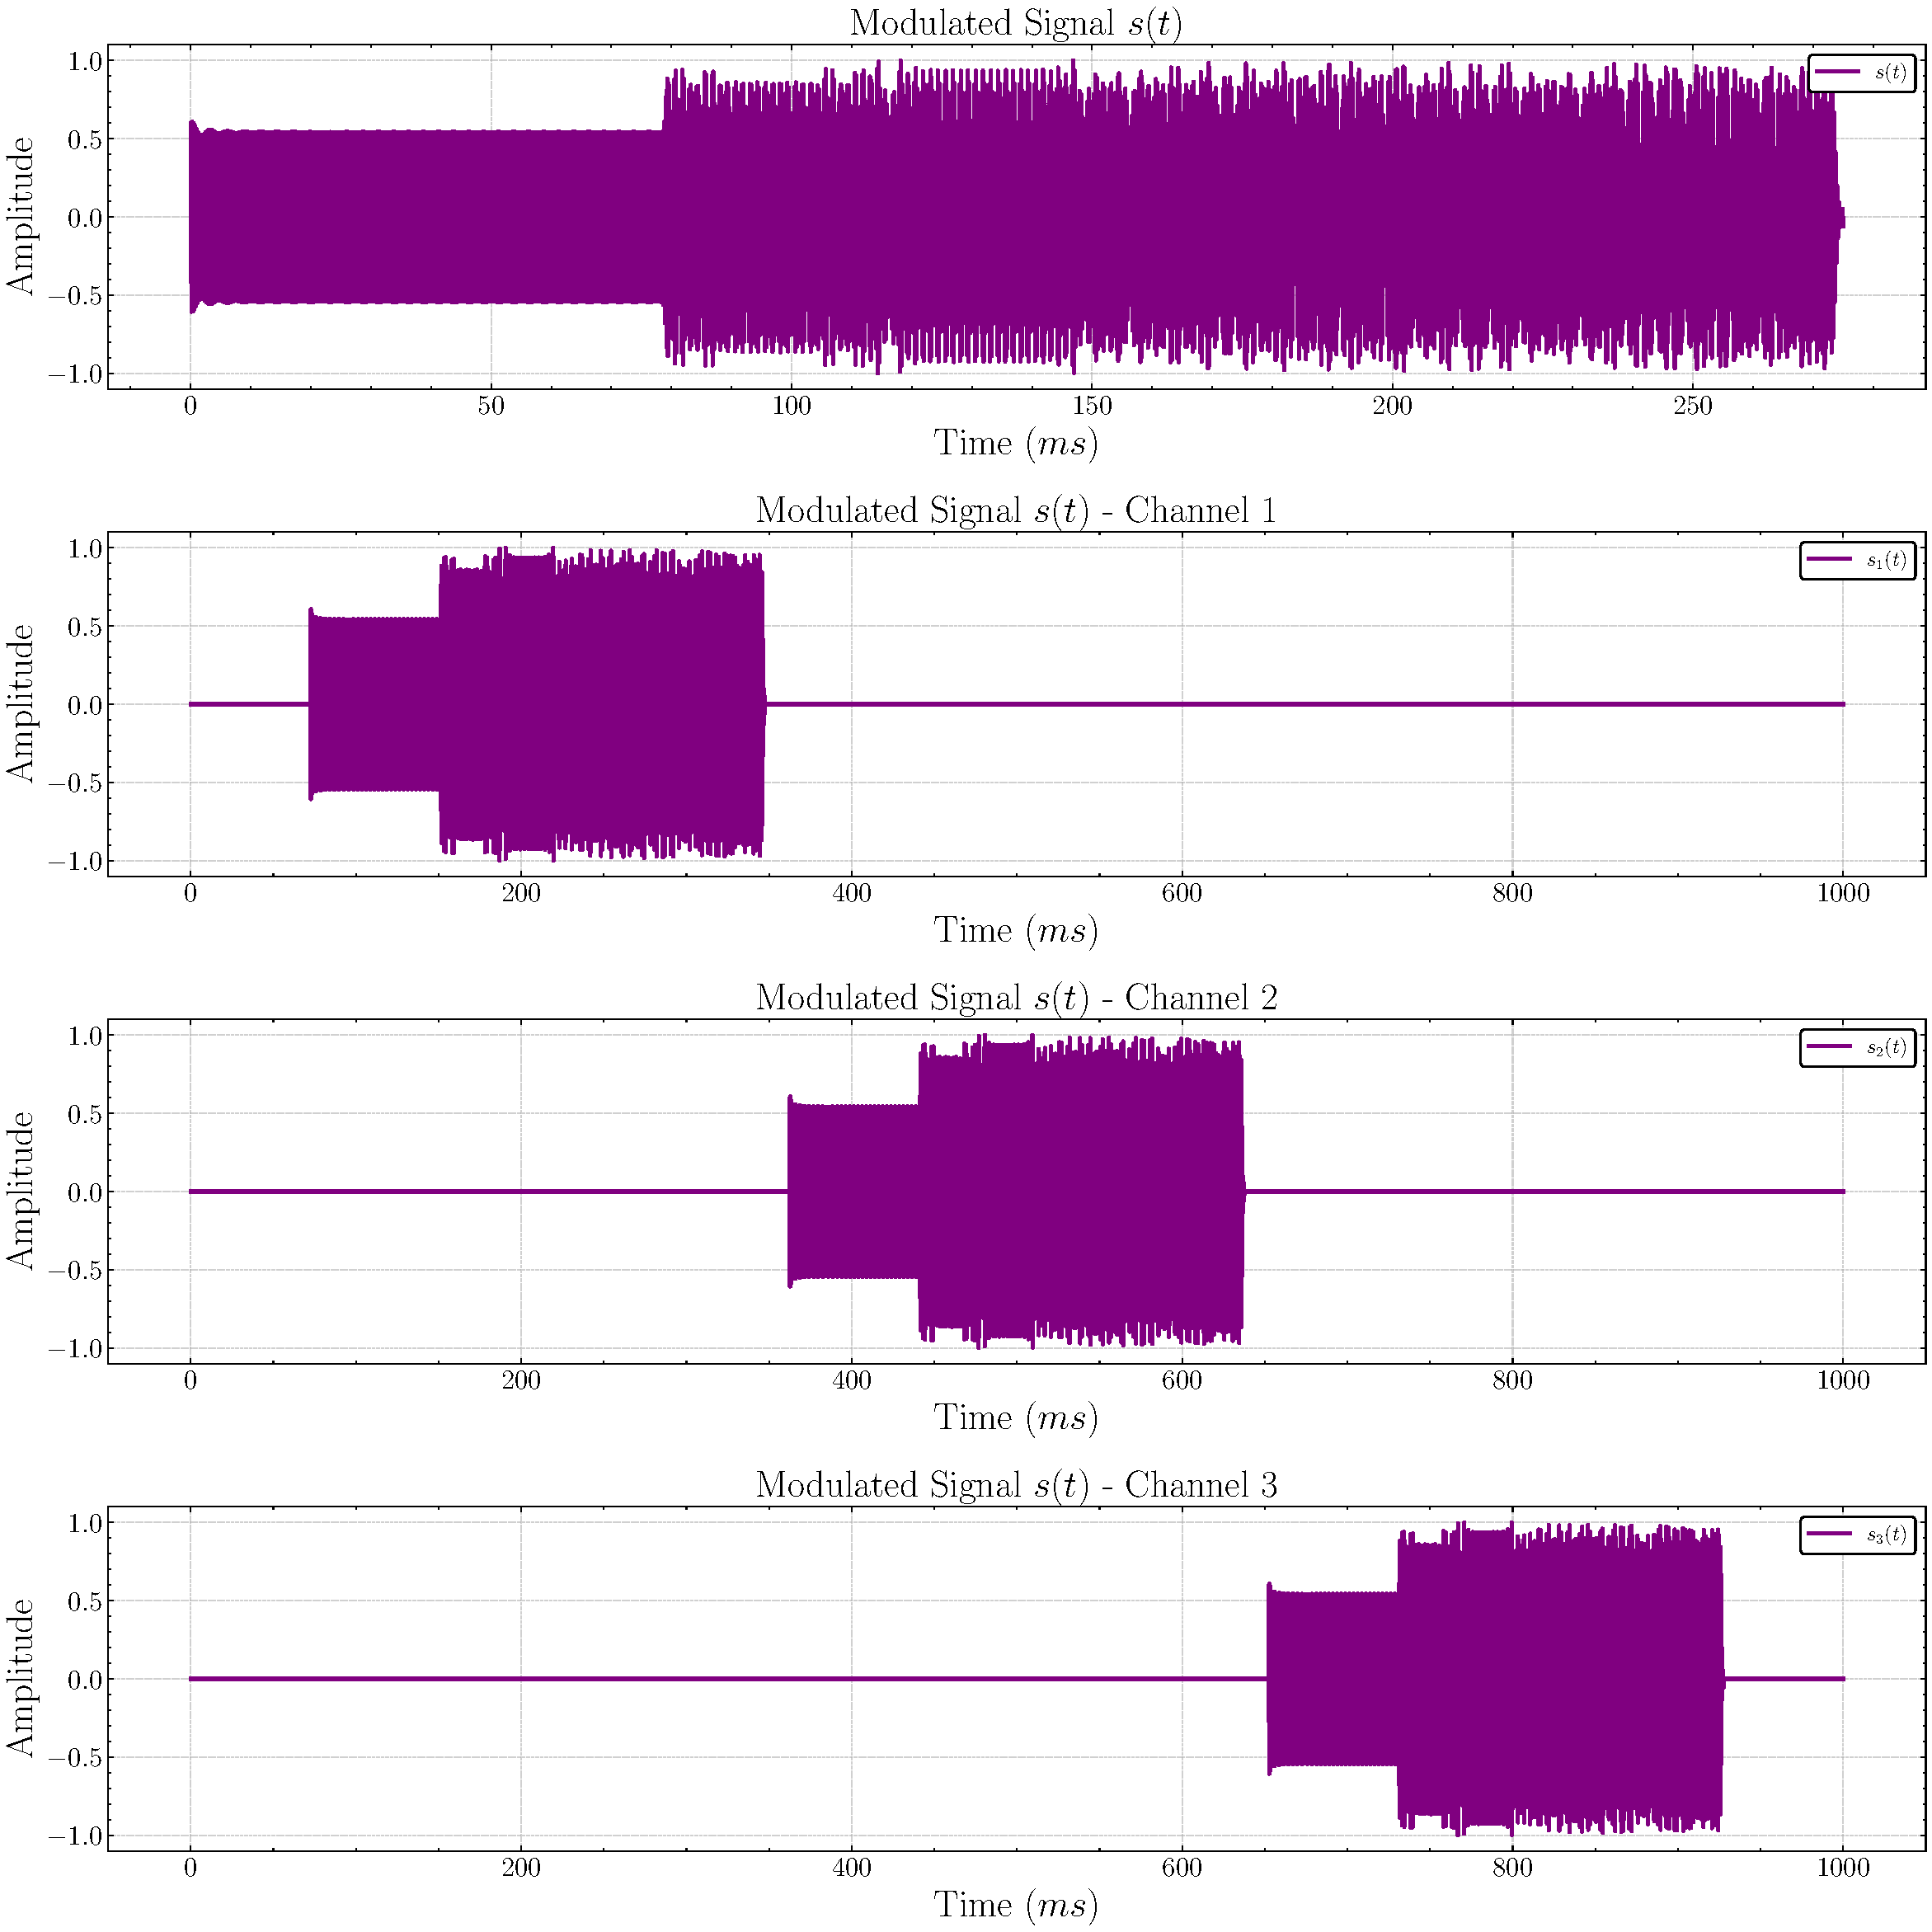
\includegraphics[width=\linewidth]{assets/cap3/example_channel_time_subchannels.pdf}
\end{figure}

\subsection{Geração de ruído AWGN}\label{sec:geracao_ruido}

\begin{figure}[H]
	\centering
	\caption{Adição de ruído ao canal}\label{fig:add_noise_time}
	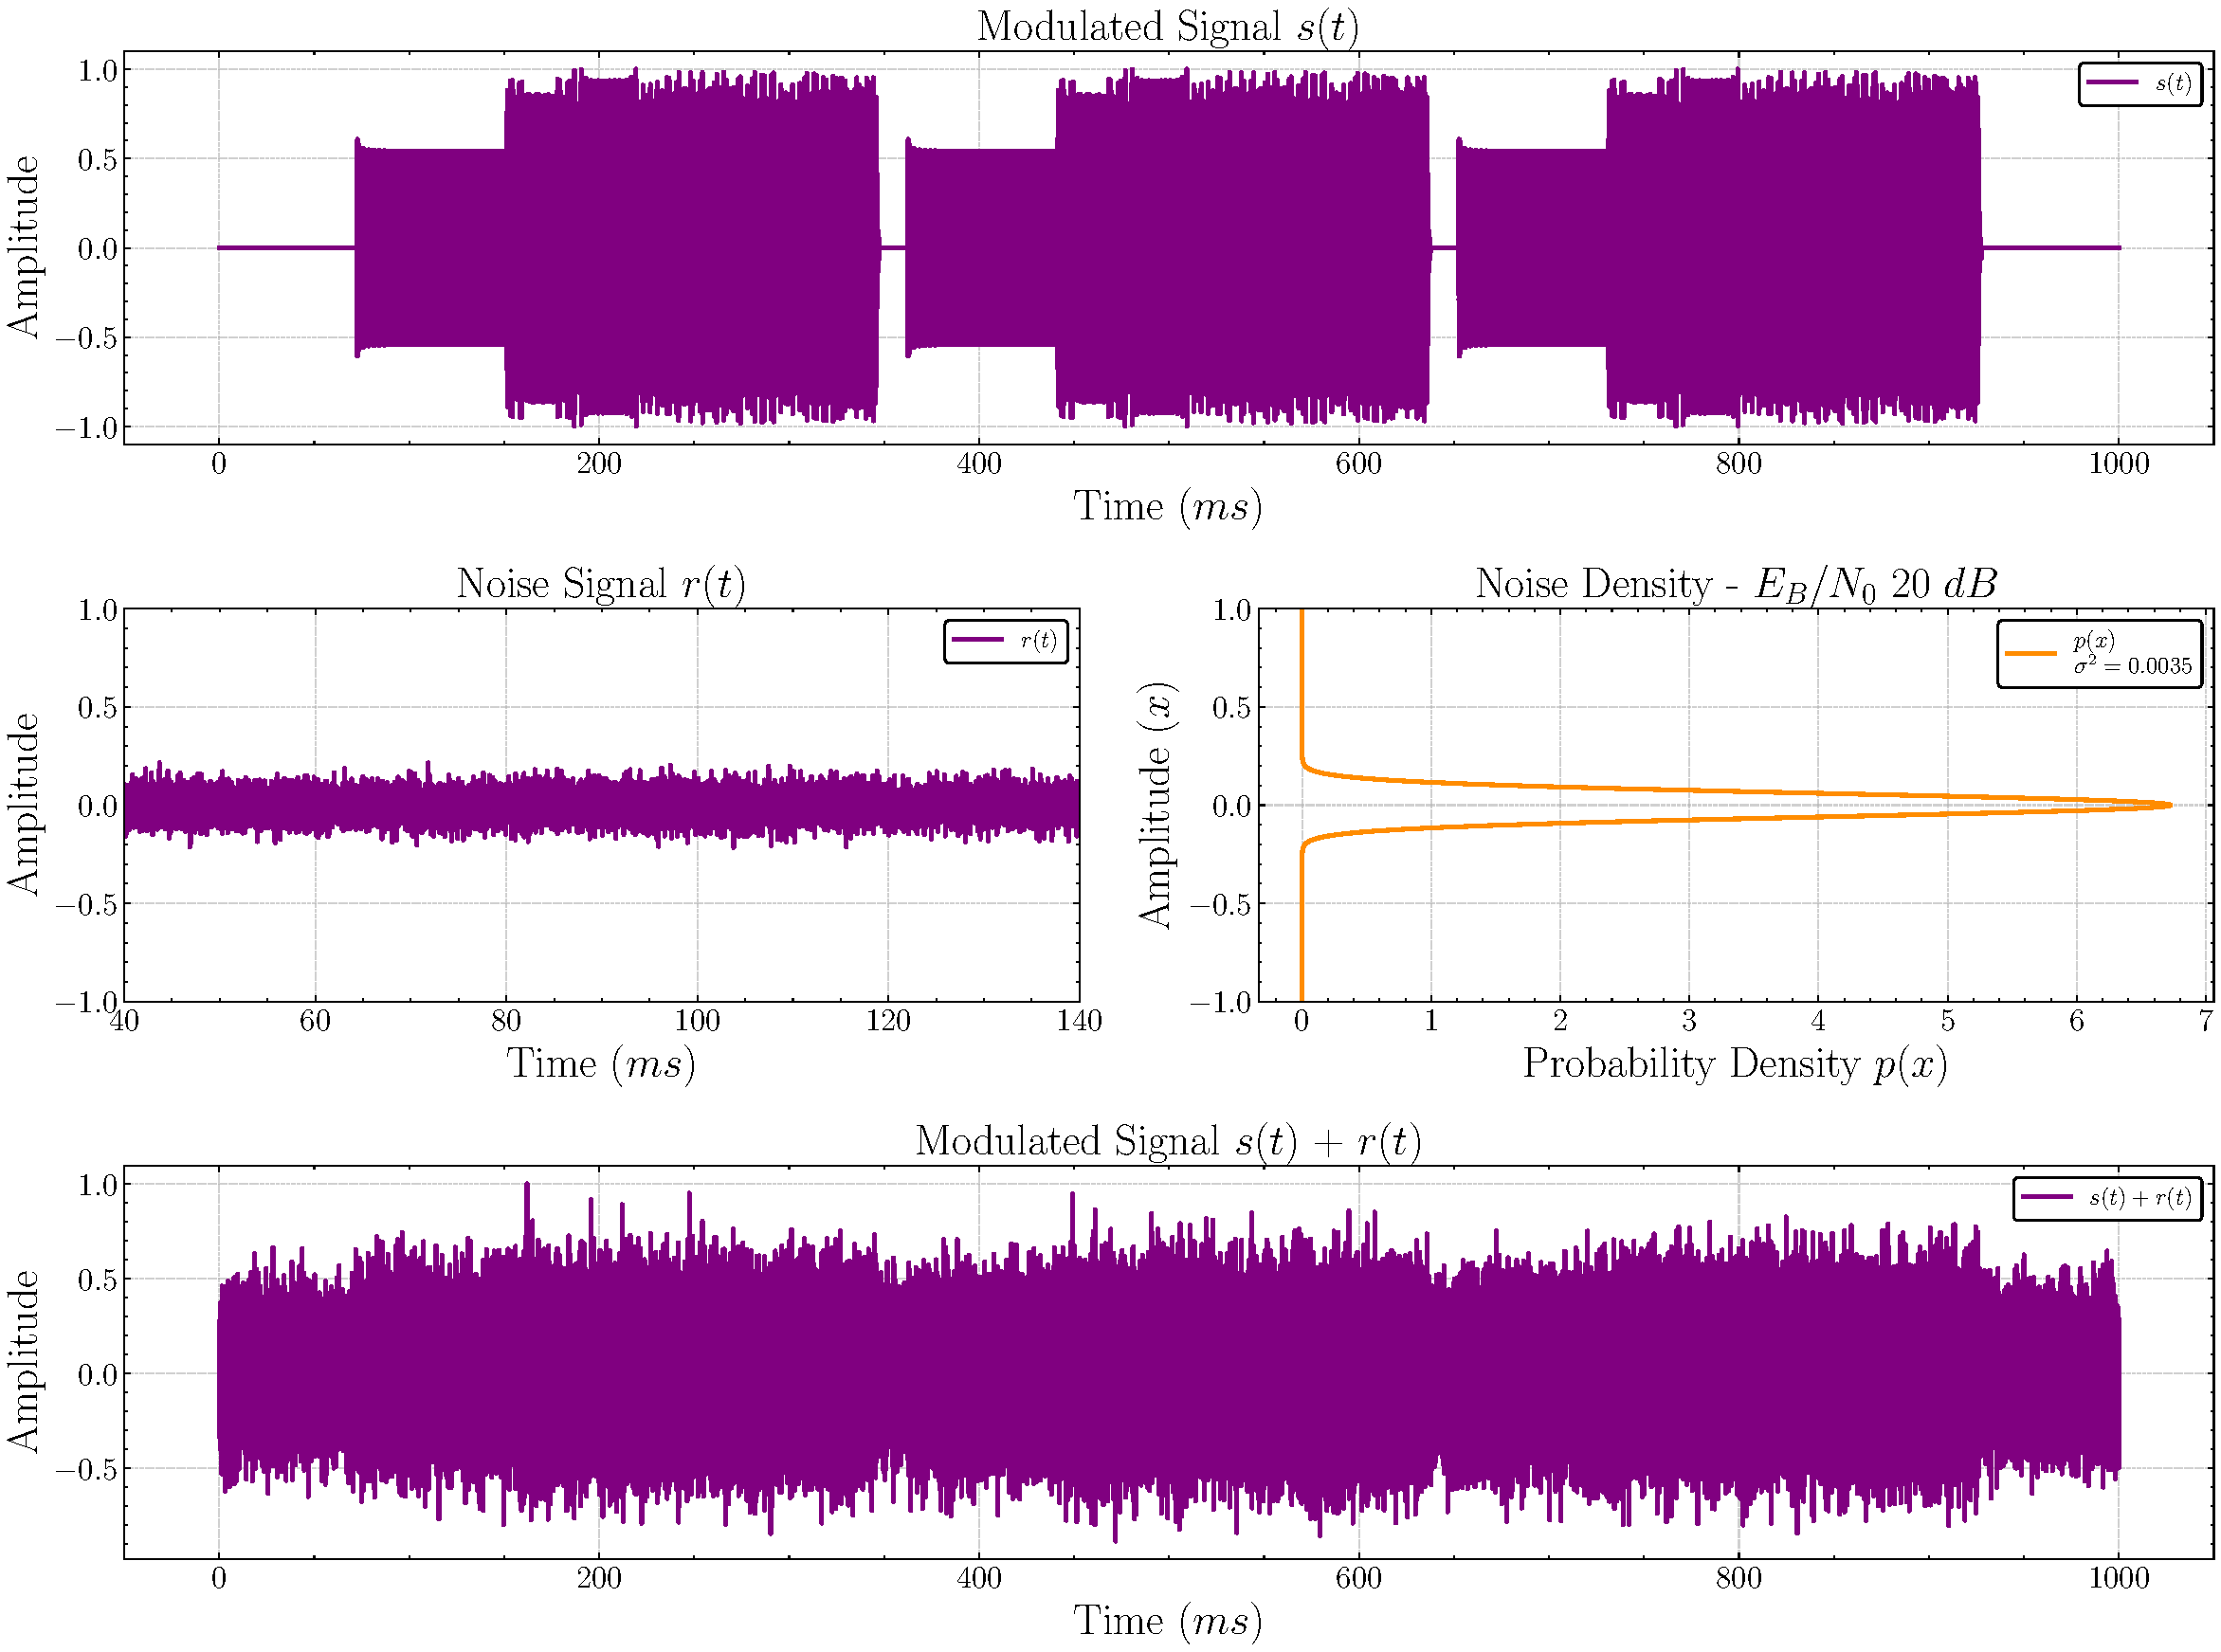
\includegraphics[width=\linewidth]{assets/cap3/example_channel_time_channel.pdf}
\end{figure}

\section{DETECÇÃO DE PORTADORA}\label{sec:detector}

\subsection{Segmentação do sinal recebido}\label{sec:segmentacao}

\begin{figure}[H]
	\centering
	\caption{Diagrama de waterfall do canal}\label{fig:waterfall}
	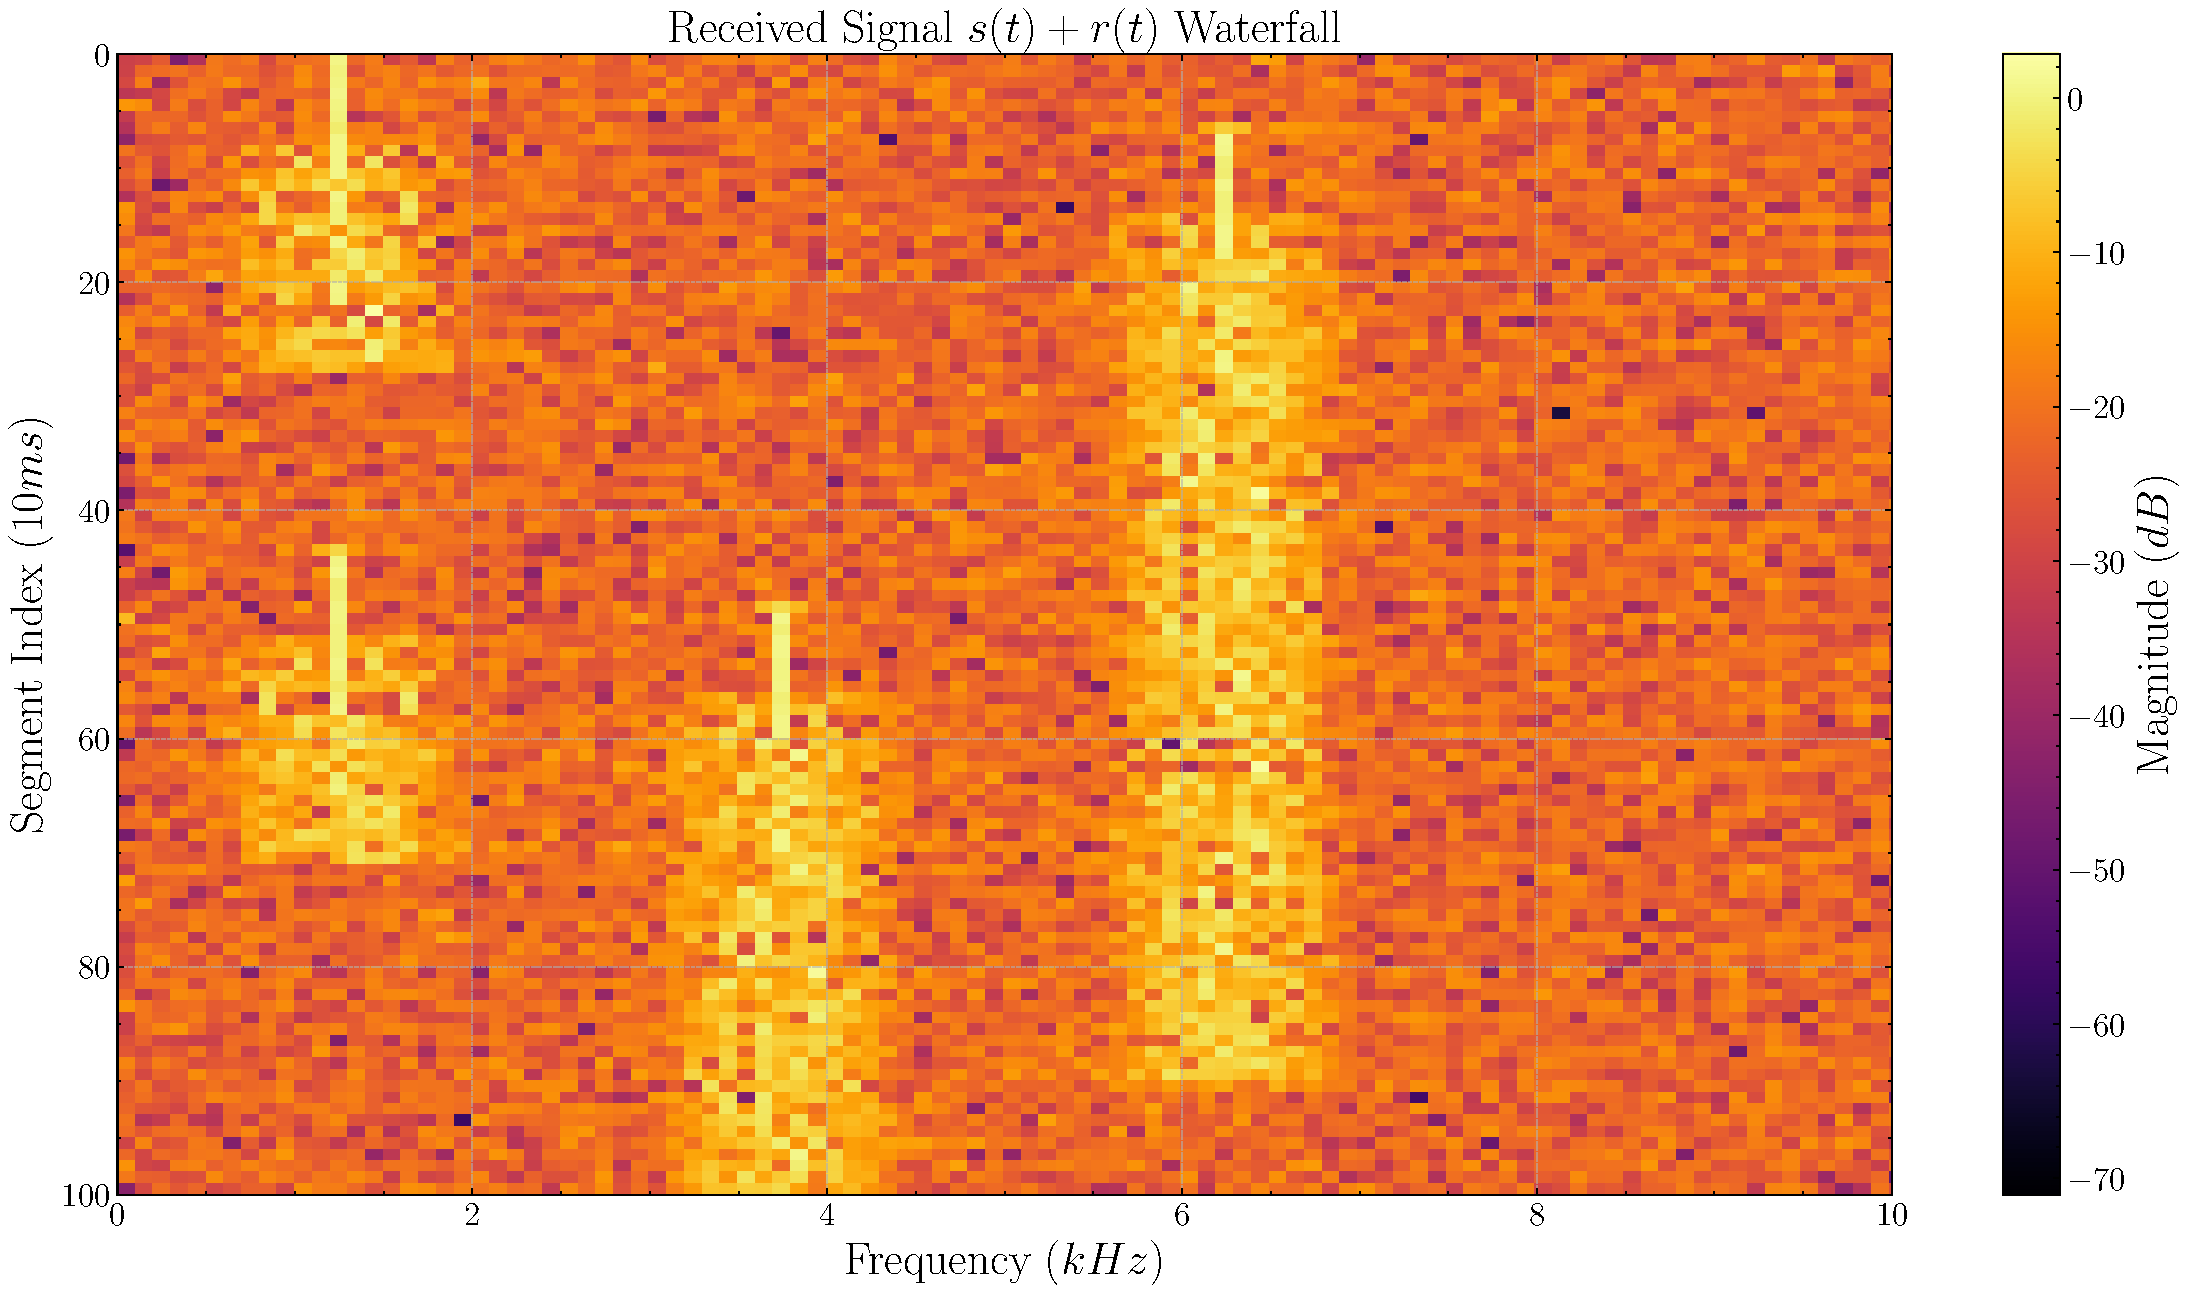
\includegraphics[width=\linewidth]{assets/cap3/example_detector_waterfall.pdf}
\end{figure}


\subsection{Detecção de componentes no espectro}\label{sec:comparacao_potencia}

\begin{figure}[H]
	\centering
	\caption{Detecção de componentes no espectro com base em $P_t$}\label{fig:freq_detection}
	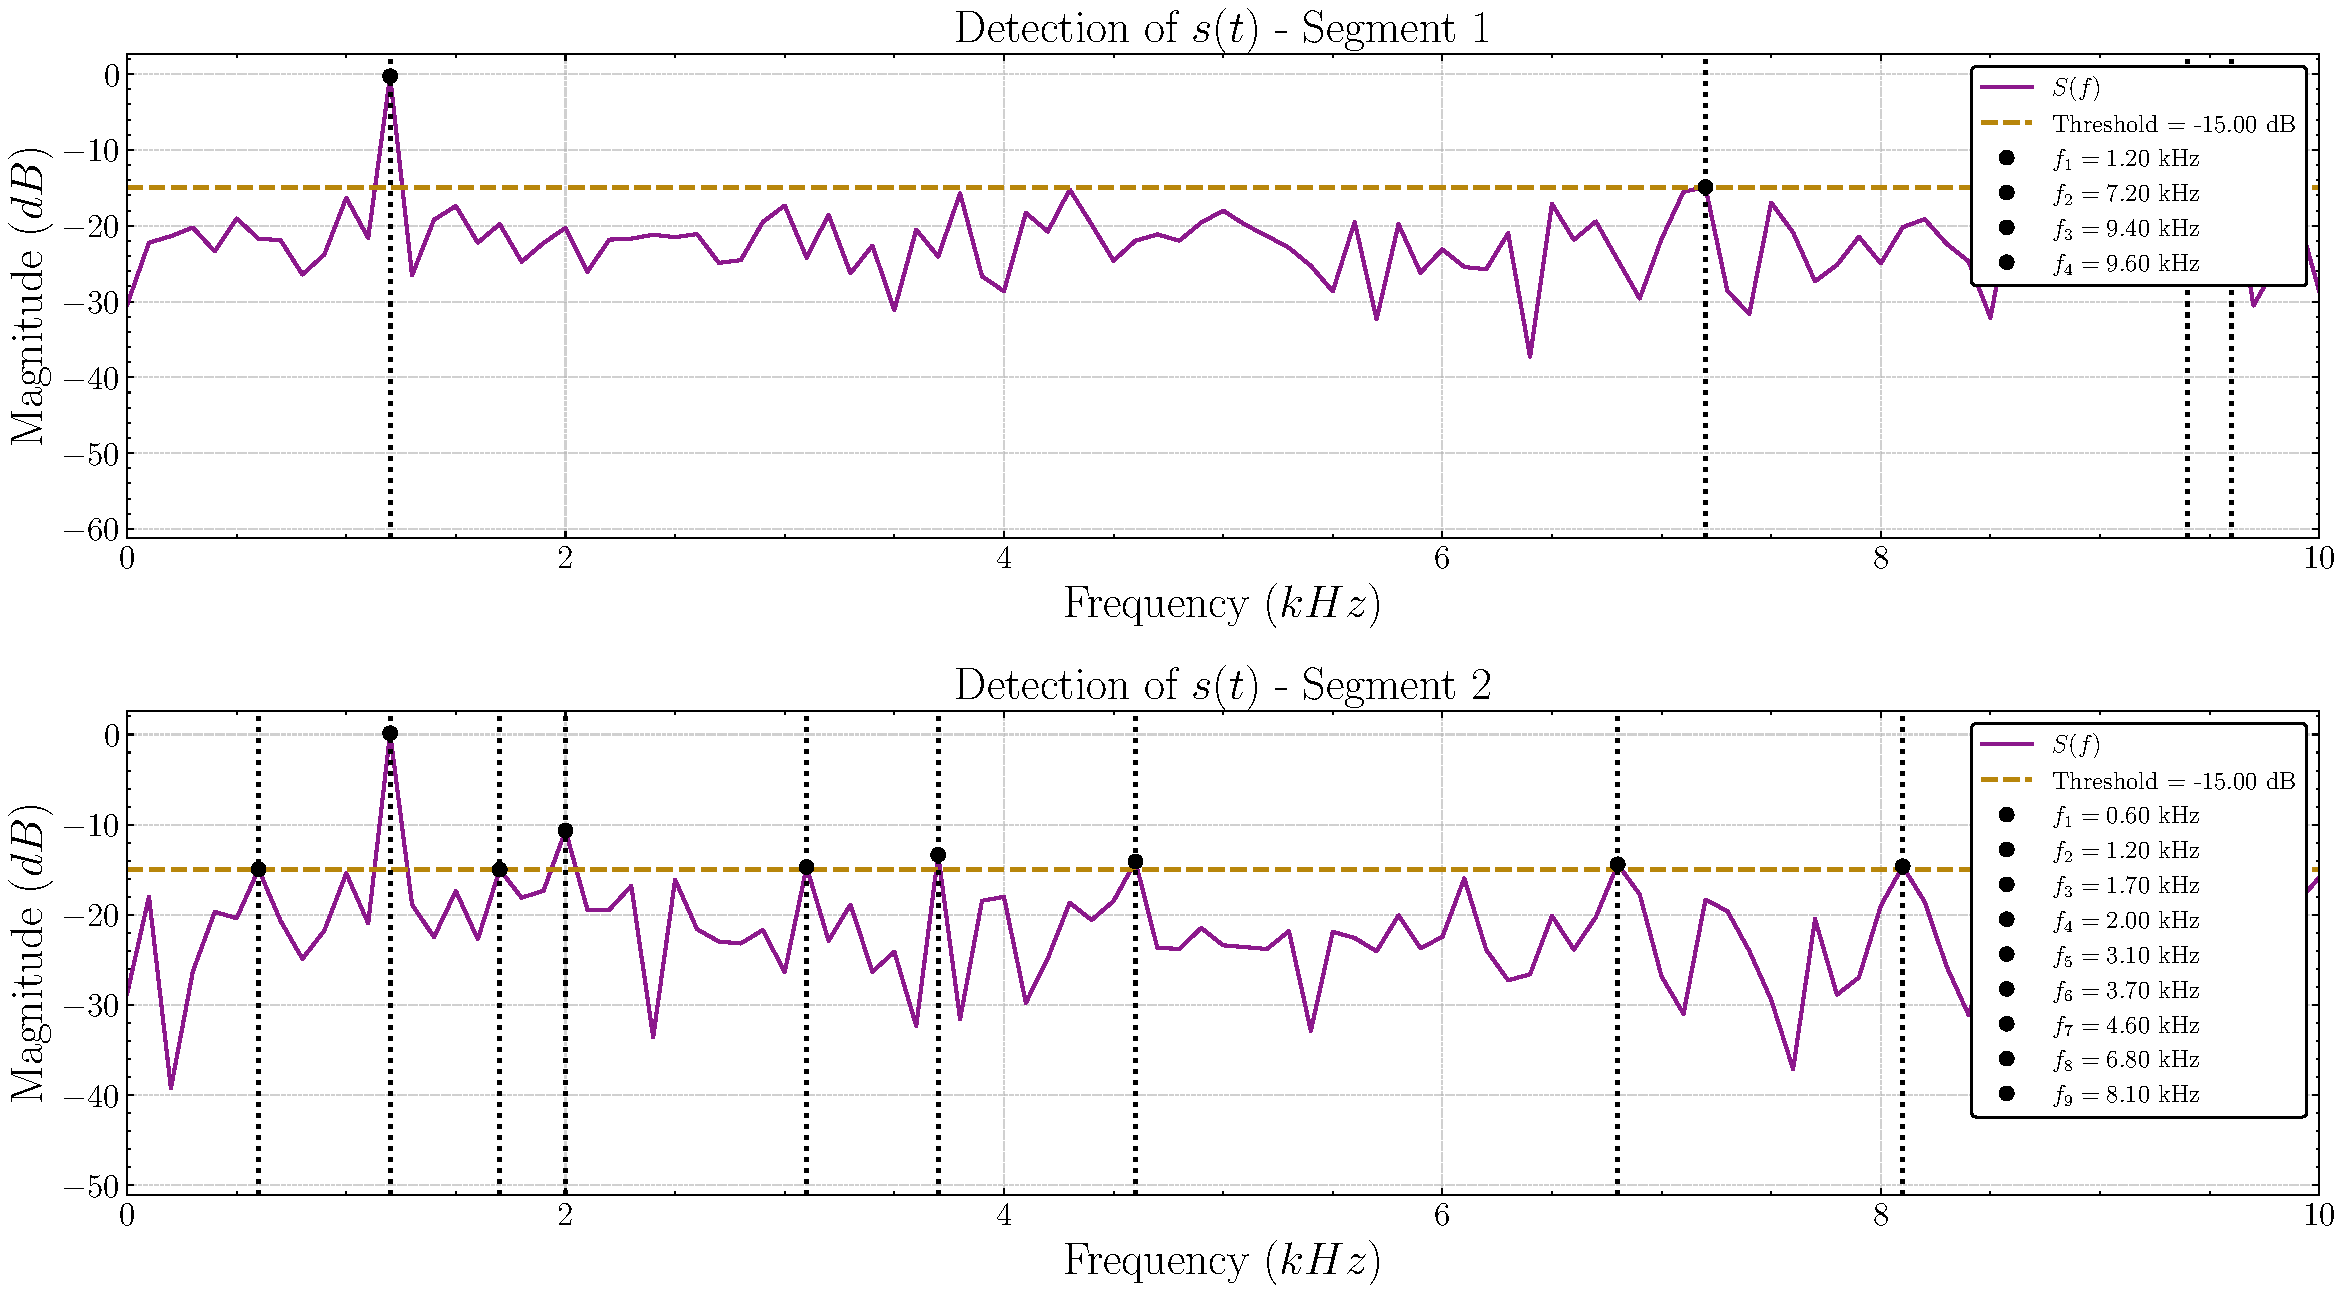
\includegraphics[width=\linewidth]{assets/cap3/example_detector_freq.pdf}
\end{figure}

\begin{figure}[H]
	\centering
	\caption{Diagrama de waterfall de detecção do canal}\label{fig:waterfall_detection}
	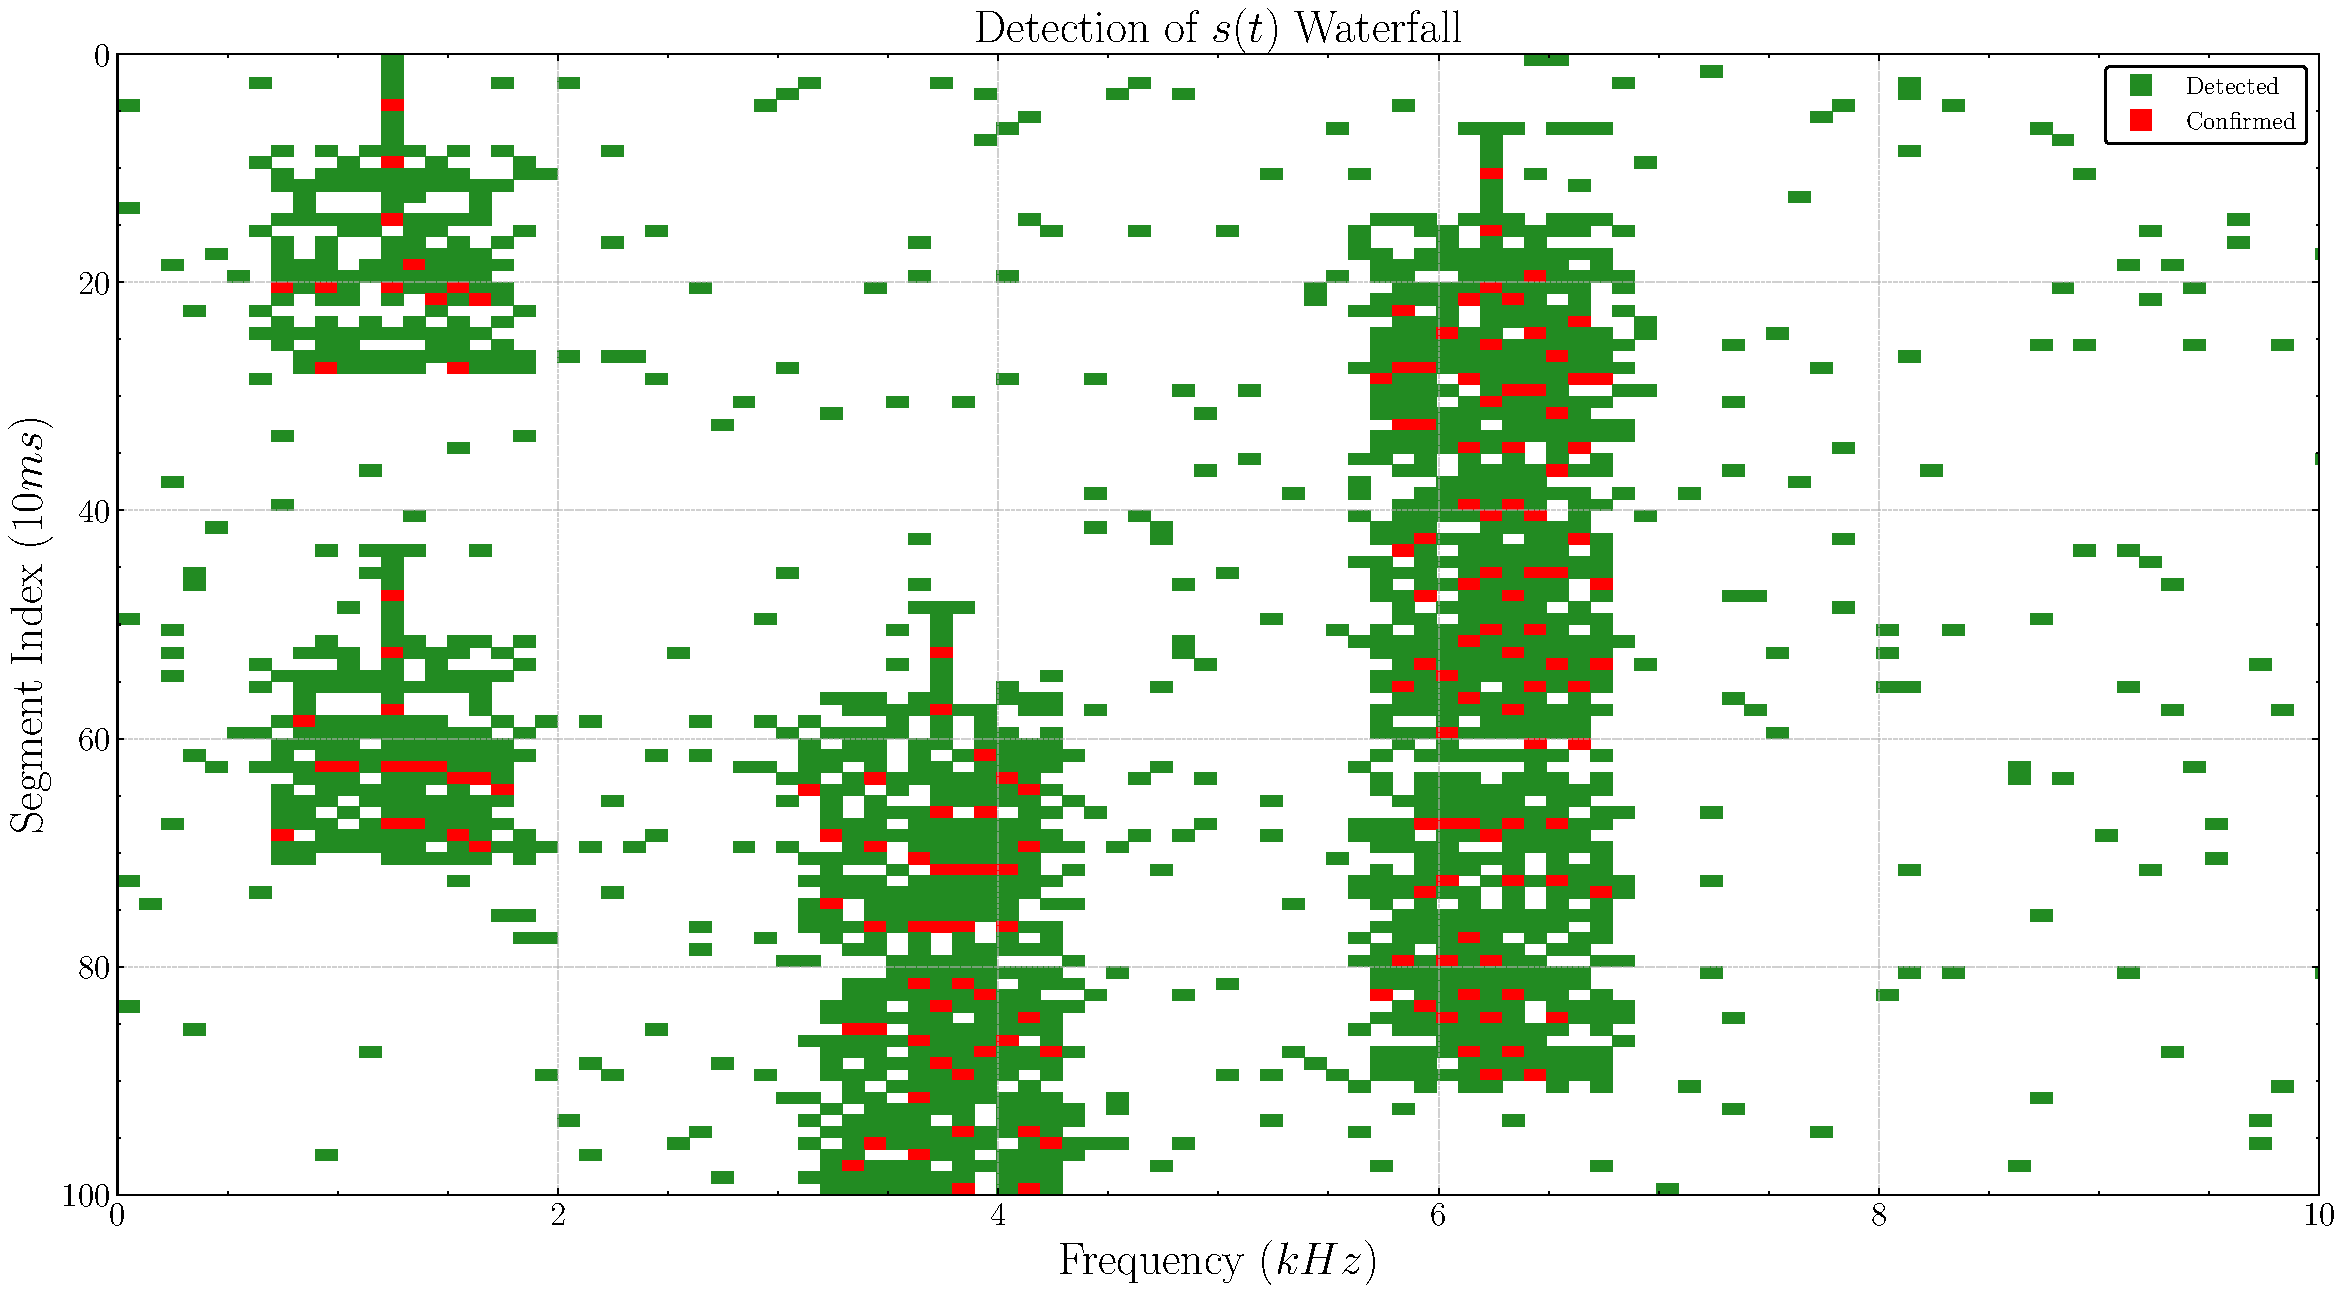
\includegraphics[width=\linewidth]{assets/cap3/example_detector_waterfall_detection.pdf}
\end{figure}


\subsection{Decisão de componentes detectadas}\label{sec:decisao}

\begin{figure}[H]
	\centering
	\caption{Diagrama de waterfall de decisão do canal}\label{fig:waterfall_decision}
	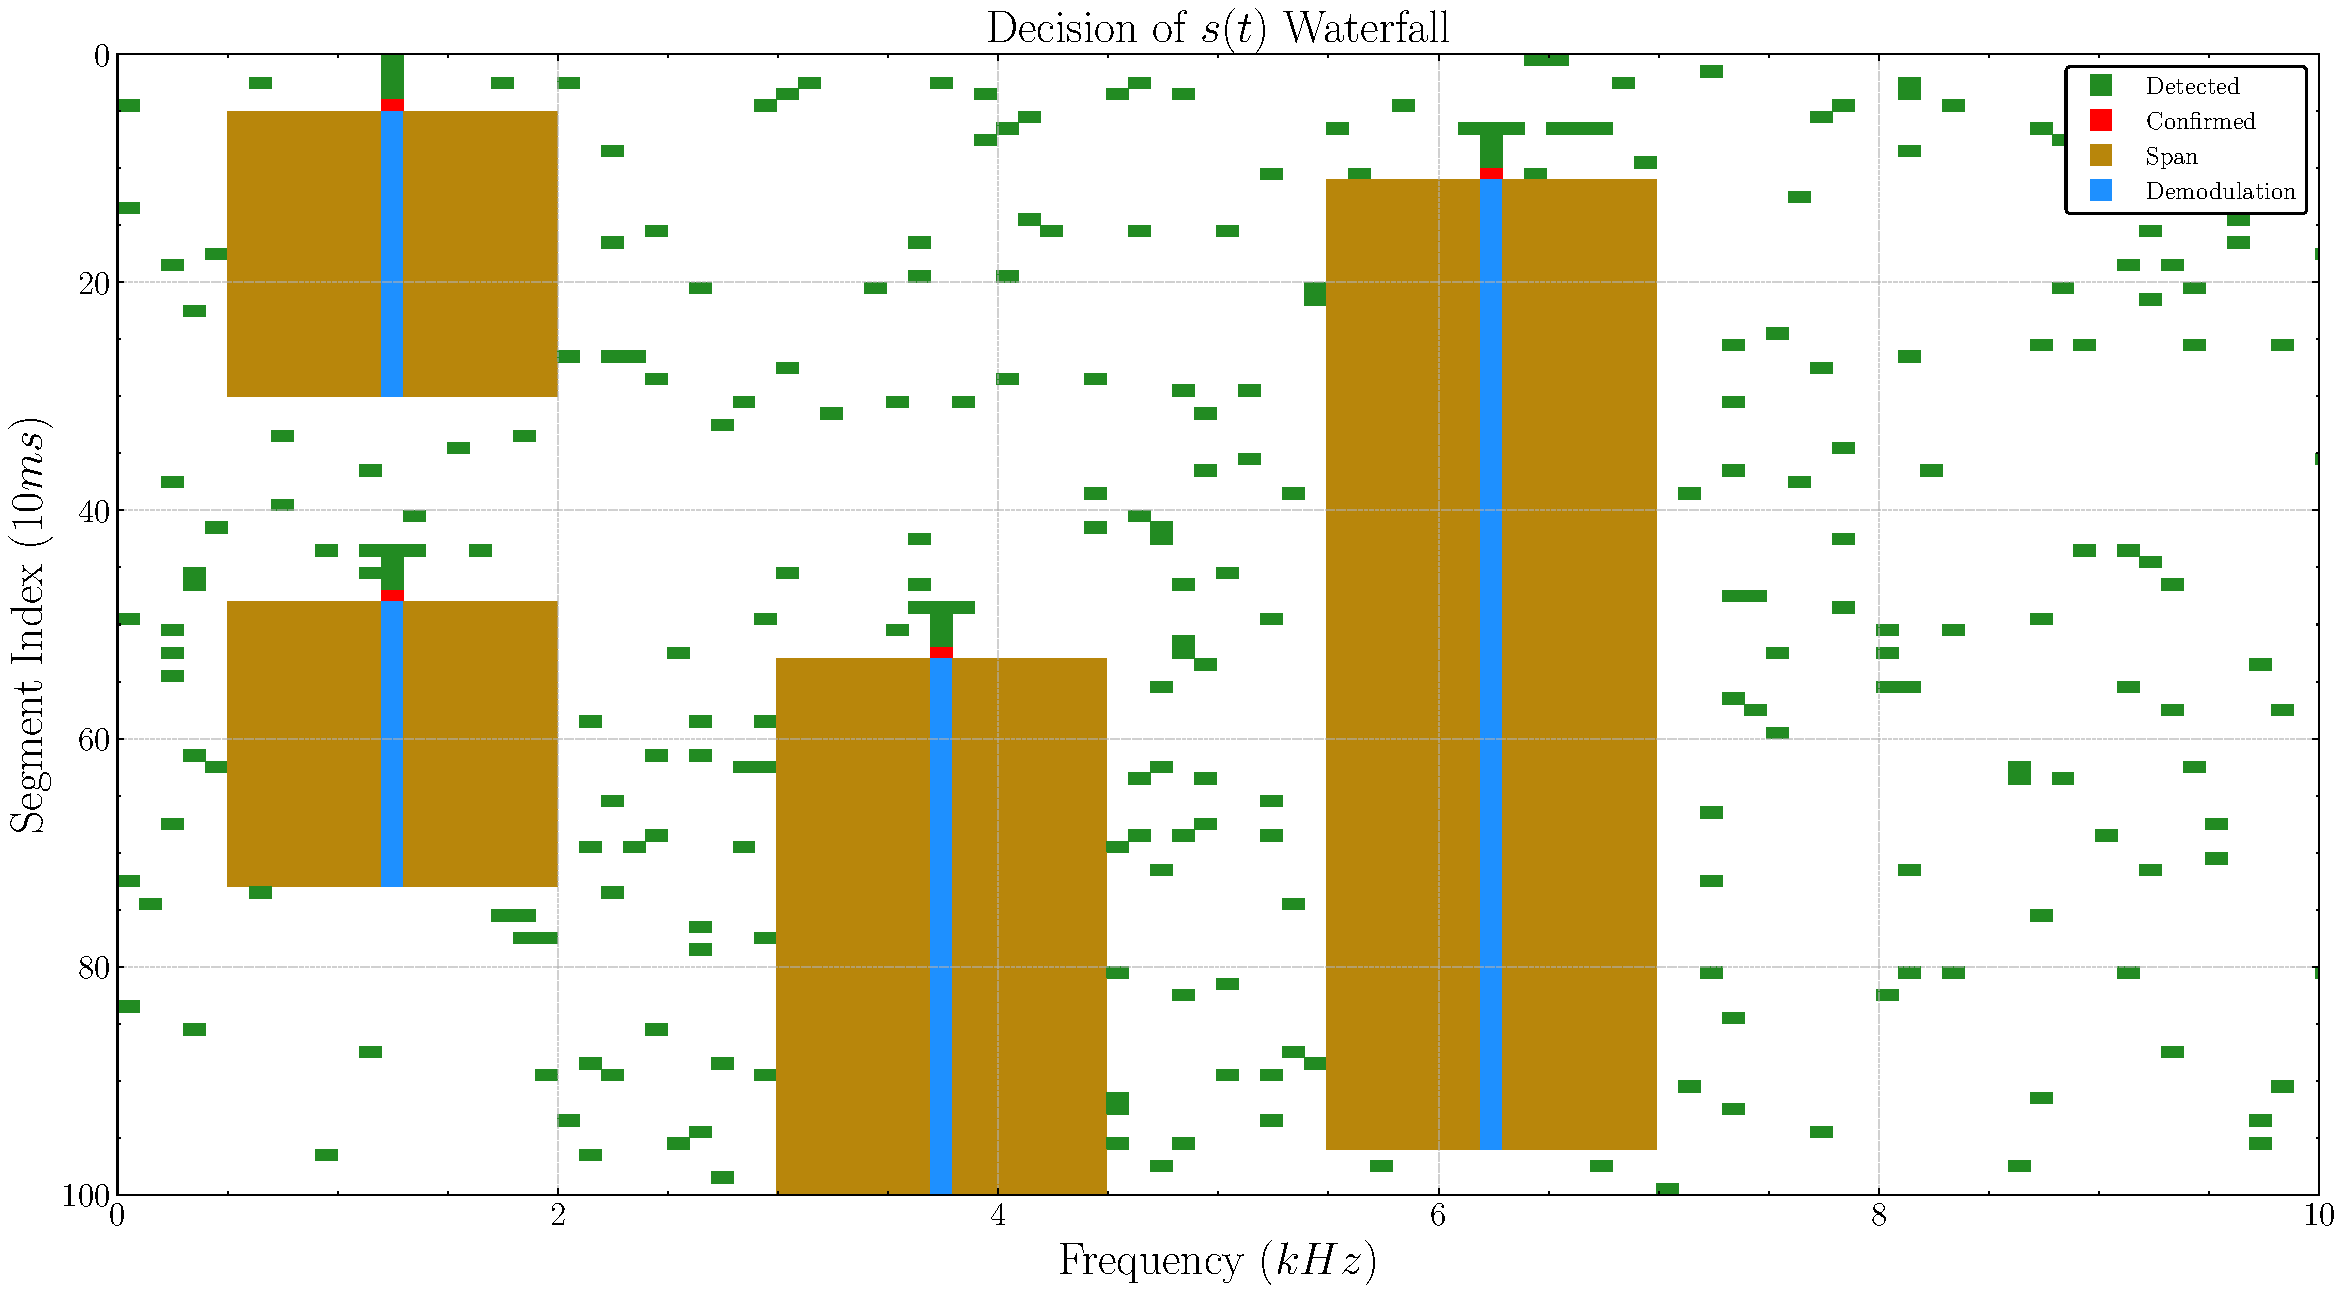
\includegraphics[width=\linewidth]{assets/cap3/example_detector_waterfall_decision.pdf}
\end{figure}

\subsection{Segmentação do sinal recebido para recepção}\label{sec:segmentacao_recepcao}

\section{CADEIA DE RECEPÇÃO}\label{sec:recepcao}    

\subsection{Demodulação banda base}\label{sec:demodulacao}

\begin{figure}[H]
	\centering
	\caption{Demodulação banda base dos canais $I$ e $Q$}\label{fig:receiver_demodulator}
	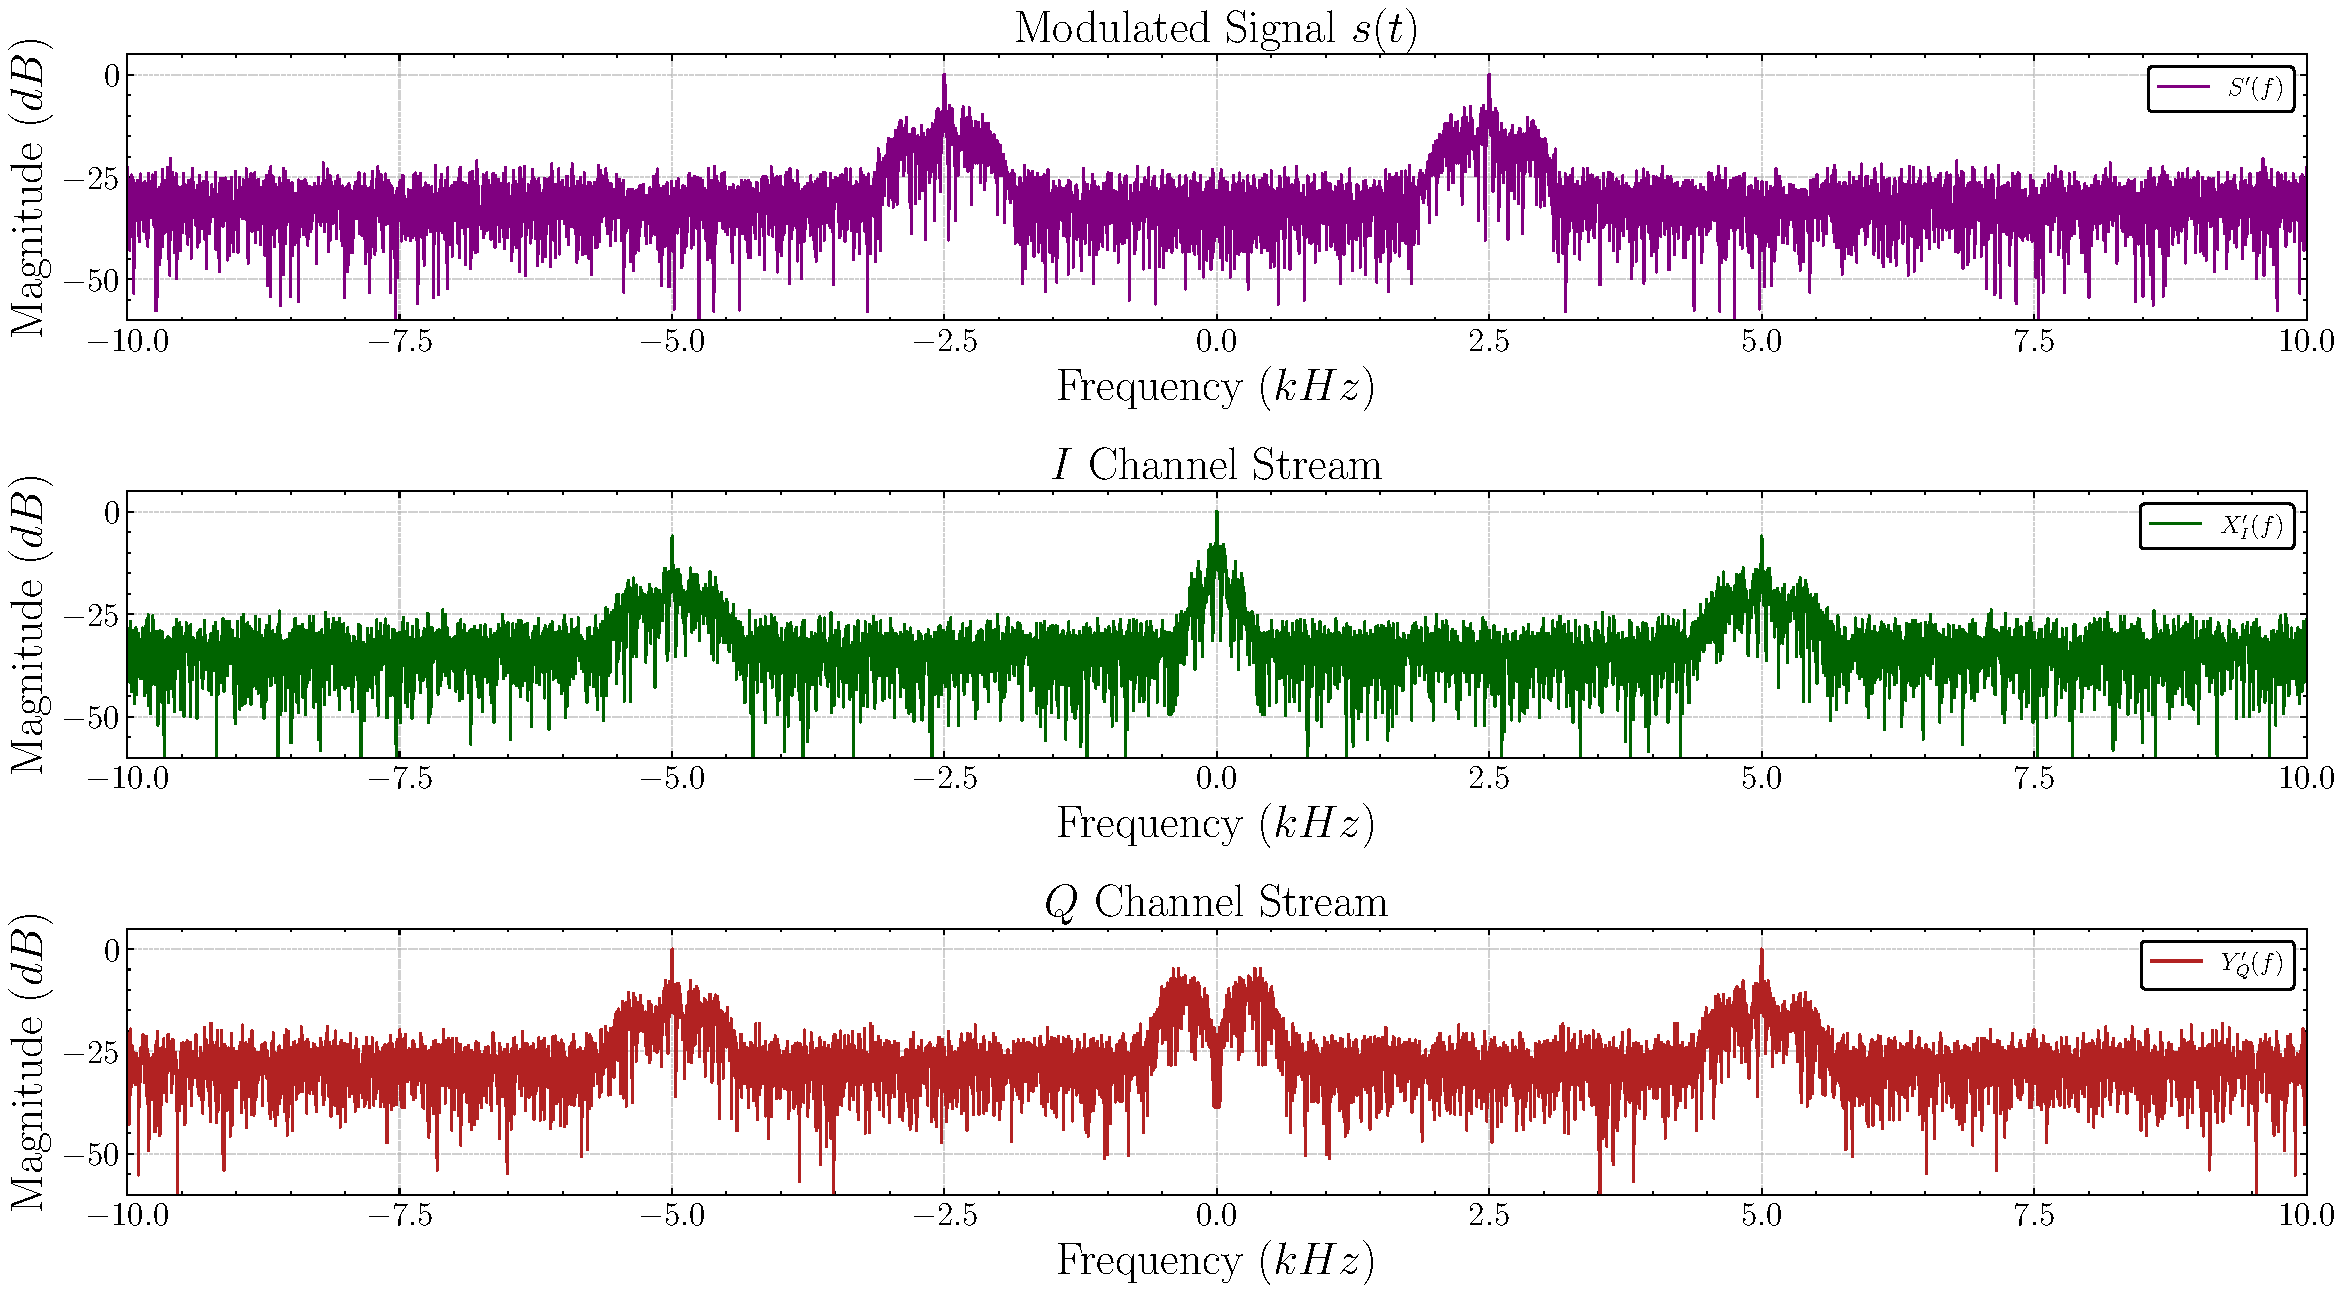
\includegraphics[width=\linewidth]{assets/cap3/receiver_demodulator_freq.pdf}
\end{figure}

\subsection{Filtragem}\label{sec:filtragem}

\begin{figure}[H]
	\centering
	\caption{Filtragem passa baixa dos canais $I$ e $Q$}\label{fig:receiver_lpf}
	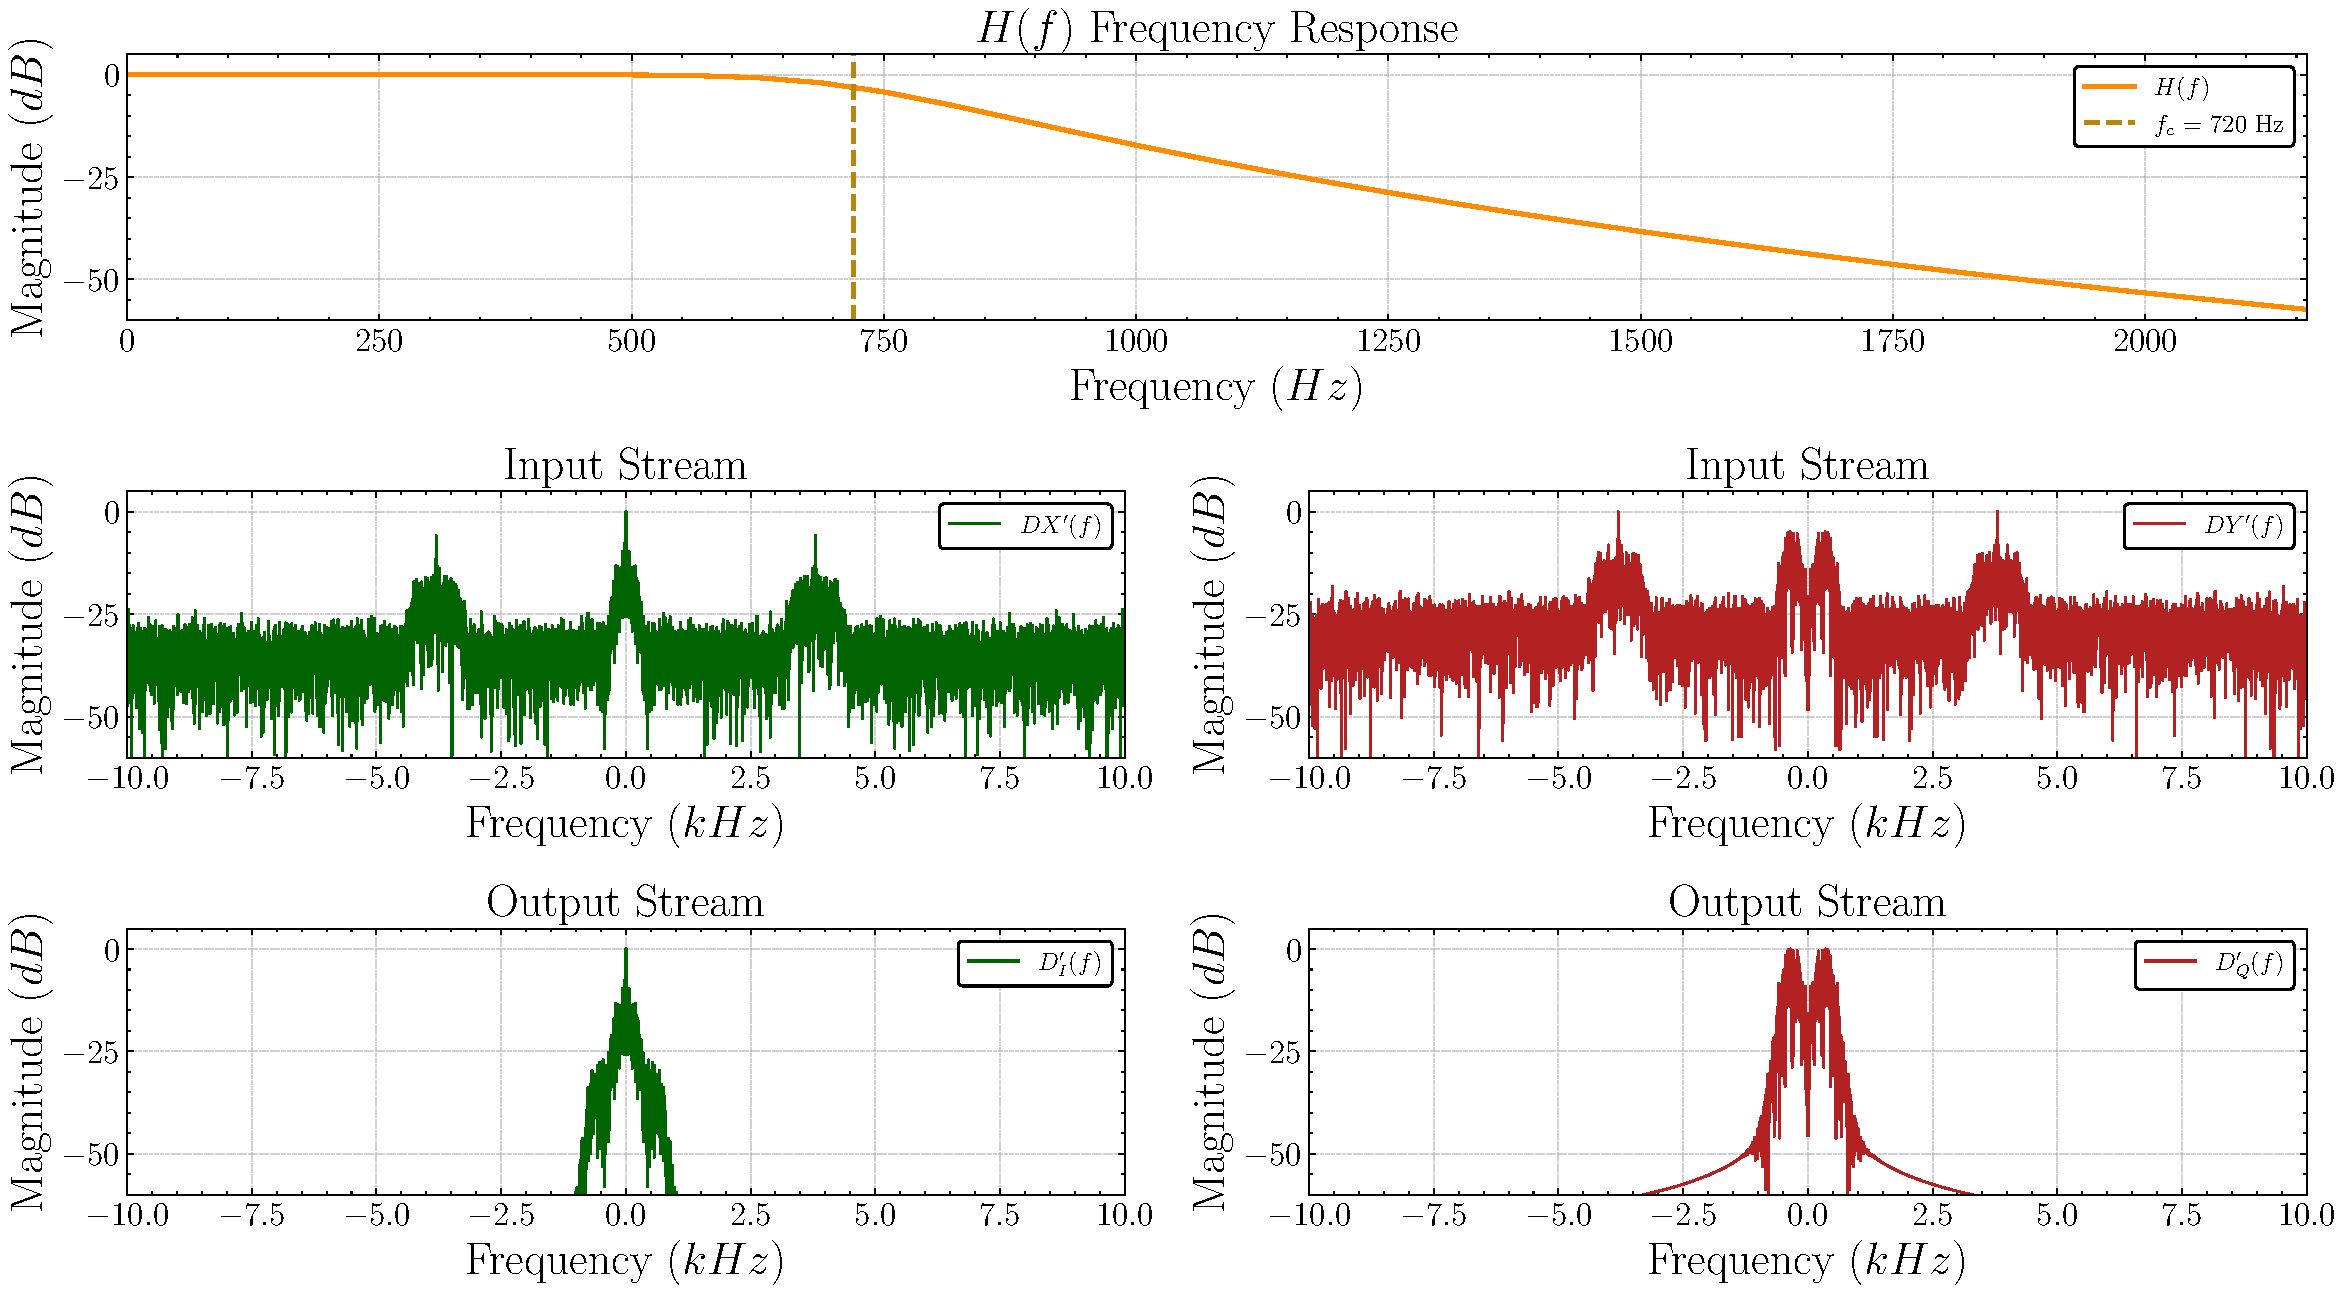
\includegraphics[width=\linewidth]{assets/cap3/receiver_lpf_freq.pdf}
\end{figure}

\begin{figure}[H]
	\centering
	\caption{Filtragem casada dos canais $I$ e $Q$}\label{fig:receiver_matchedfilter}
	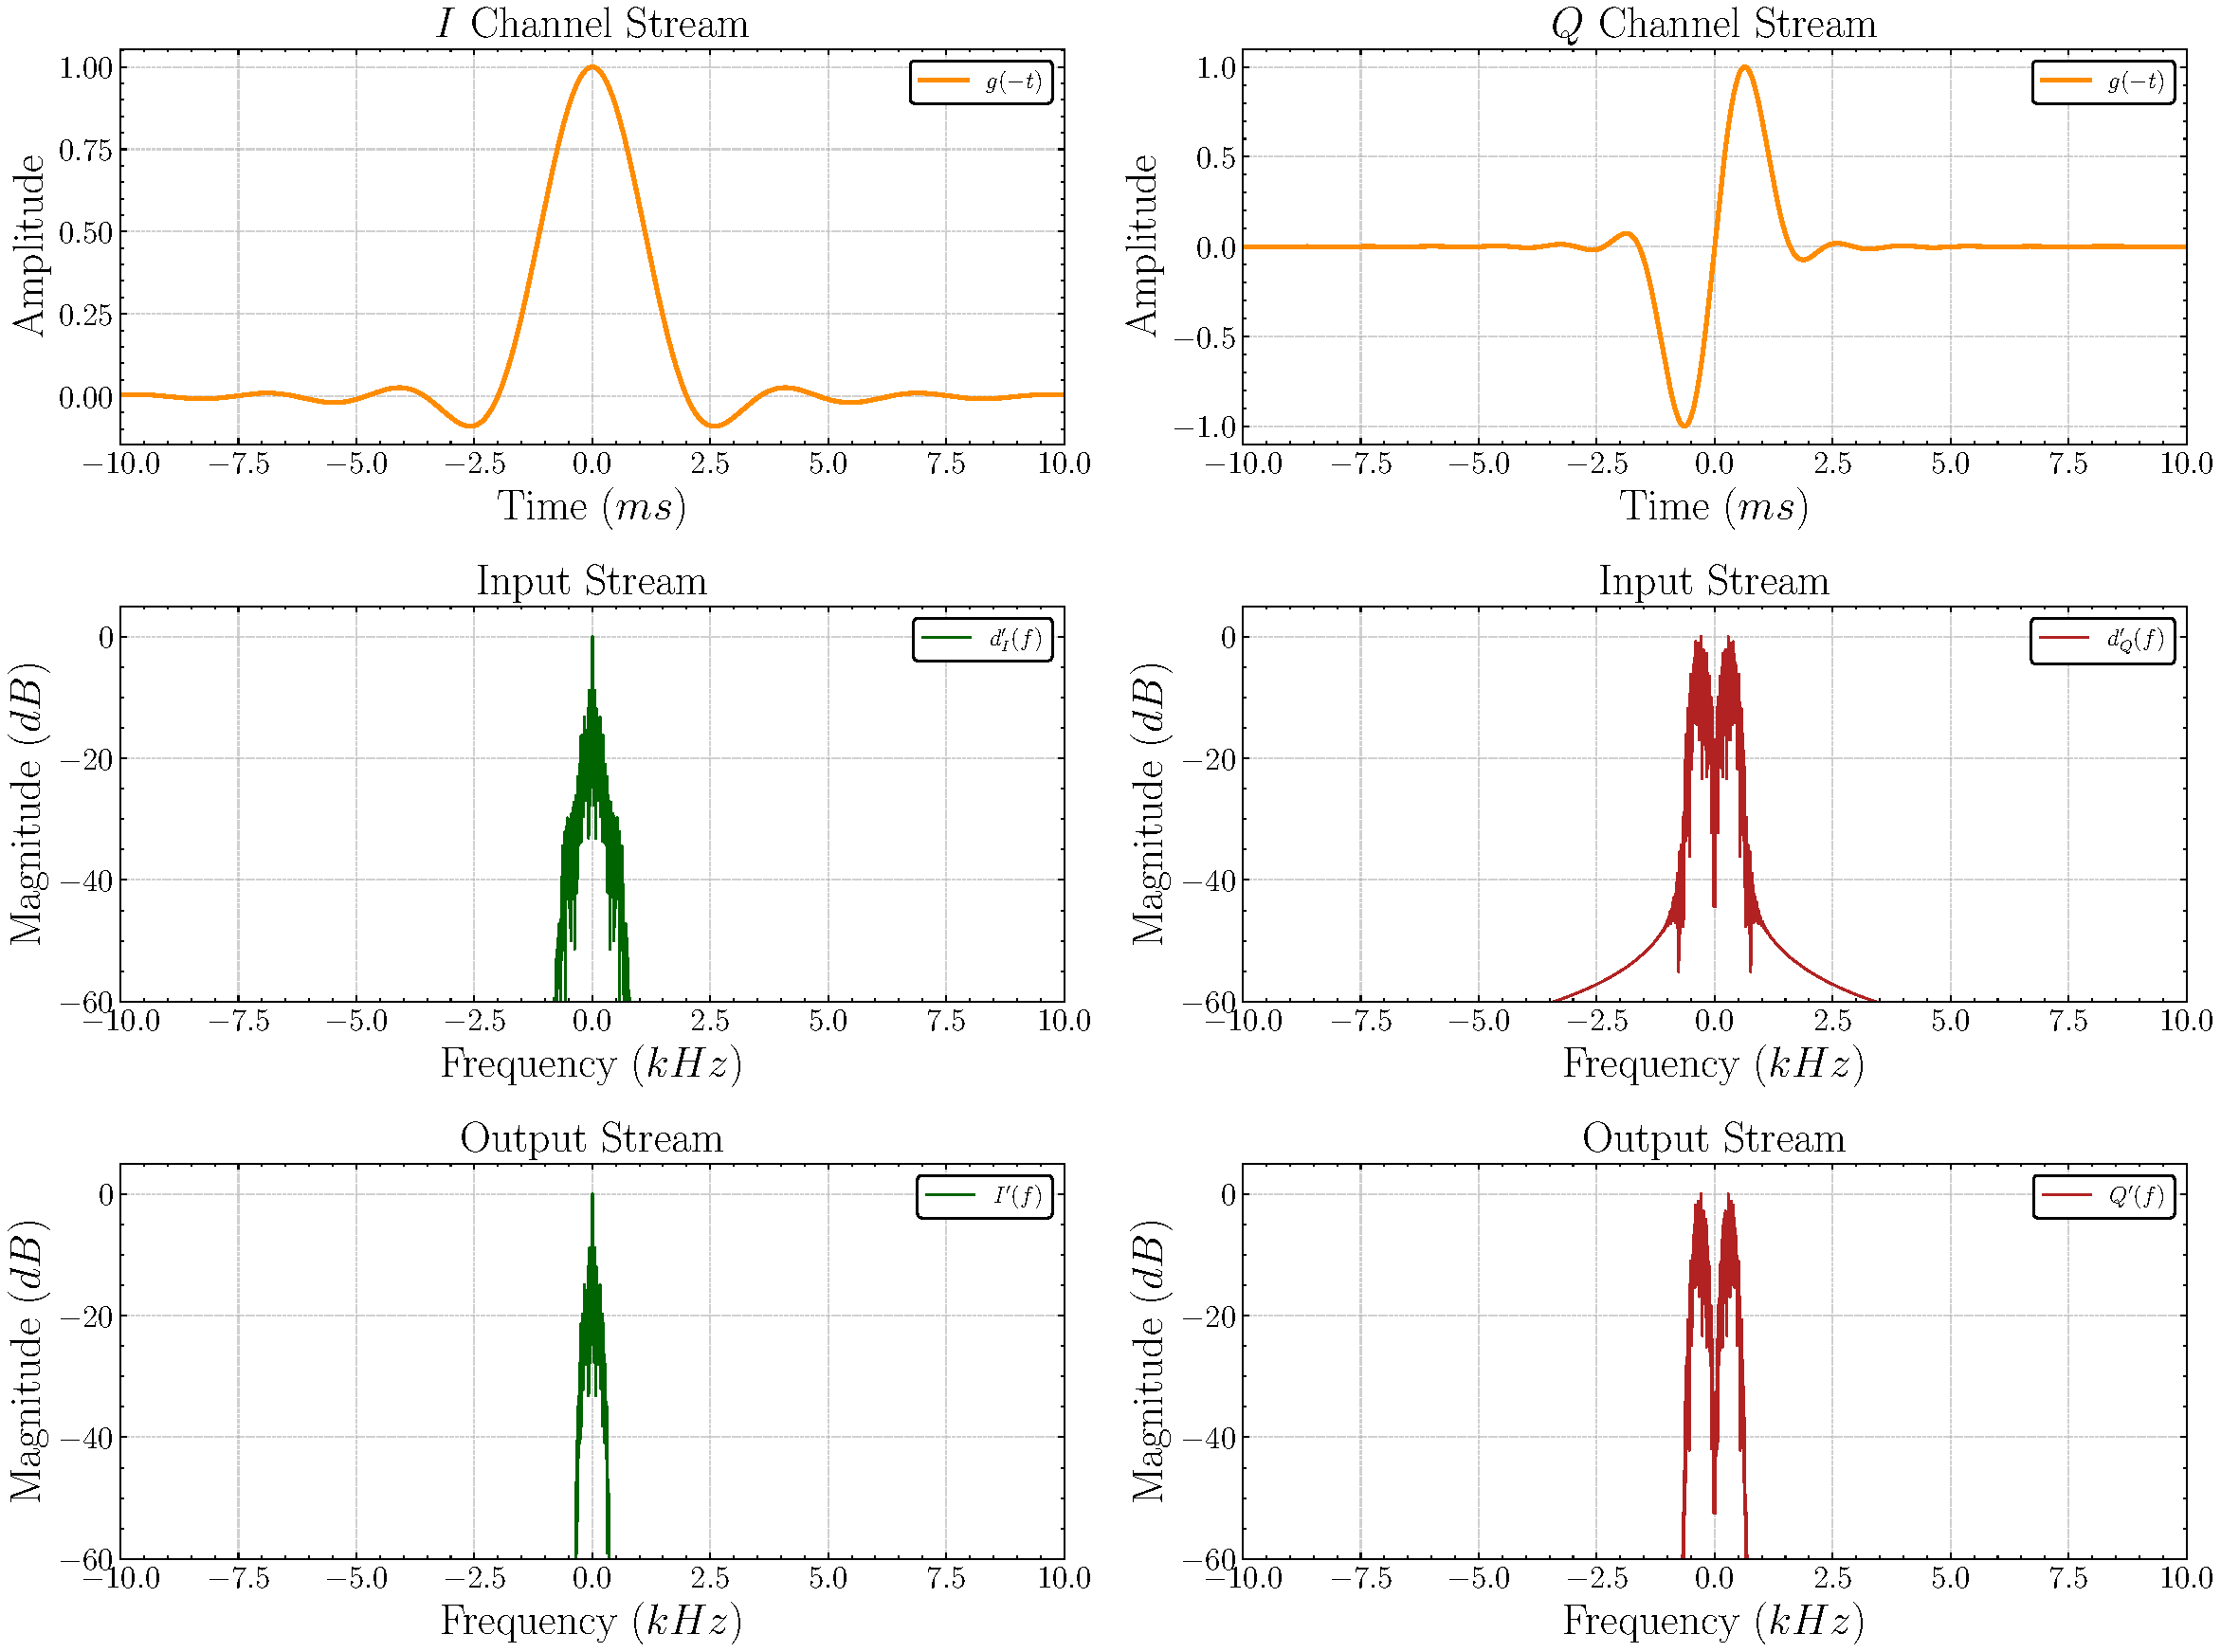
\includegraphics[width=\linewidth]{assets/cap3/receiver_mf_freq.pdf}
\end{figure}

\subsection{Sincronização de símbolos}\label{sec:sincronizacao}

\begin{figure}[H]
	\centering
	\caption{Vetor de amostras esperadas para sincronismo com $I$ e $Q$}\label{fig:receiver_sync_word}
	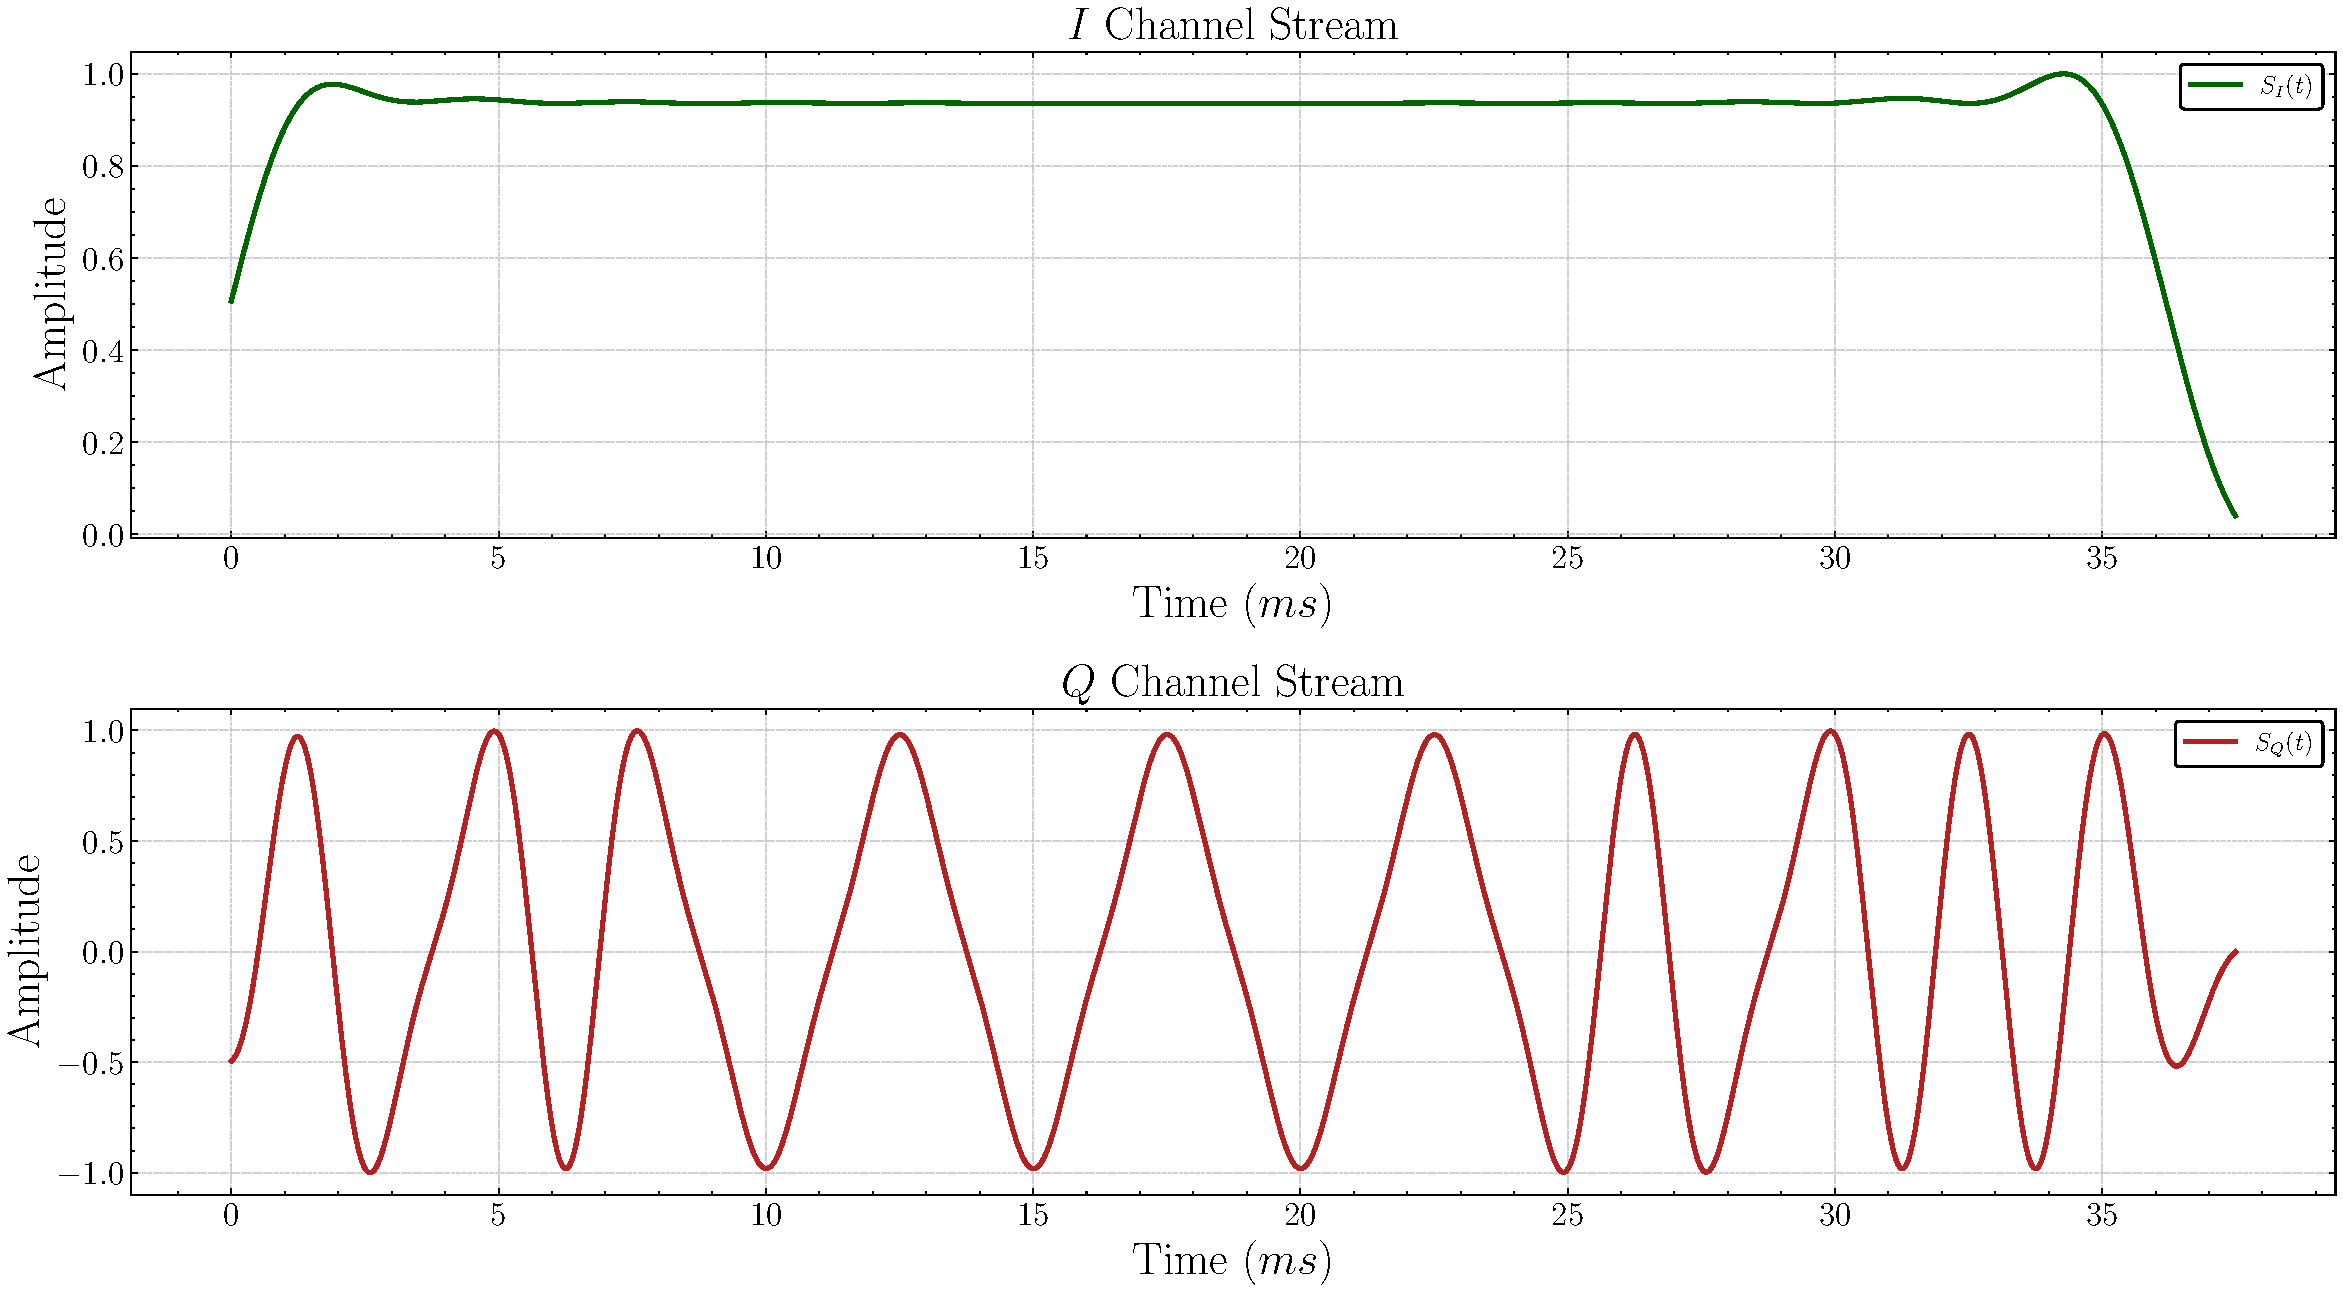
\includegraphics[width=\linewidth]{assets/cap3/example_synchronizer_word.pdf}
\end{figure}

\begin{figure}[H]
	\centering
	\caption{Módulo de correlação entre $I$ e $Q$ e vetor de sincronismo}\label{fig:receiver_corr}
	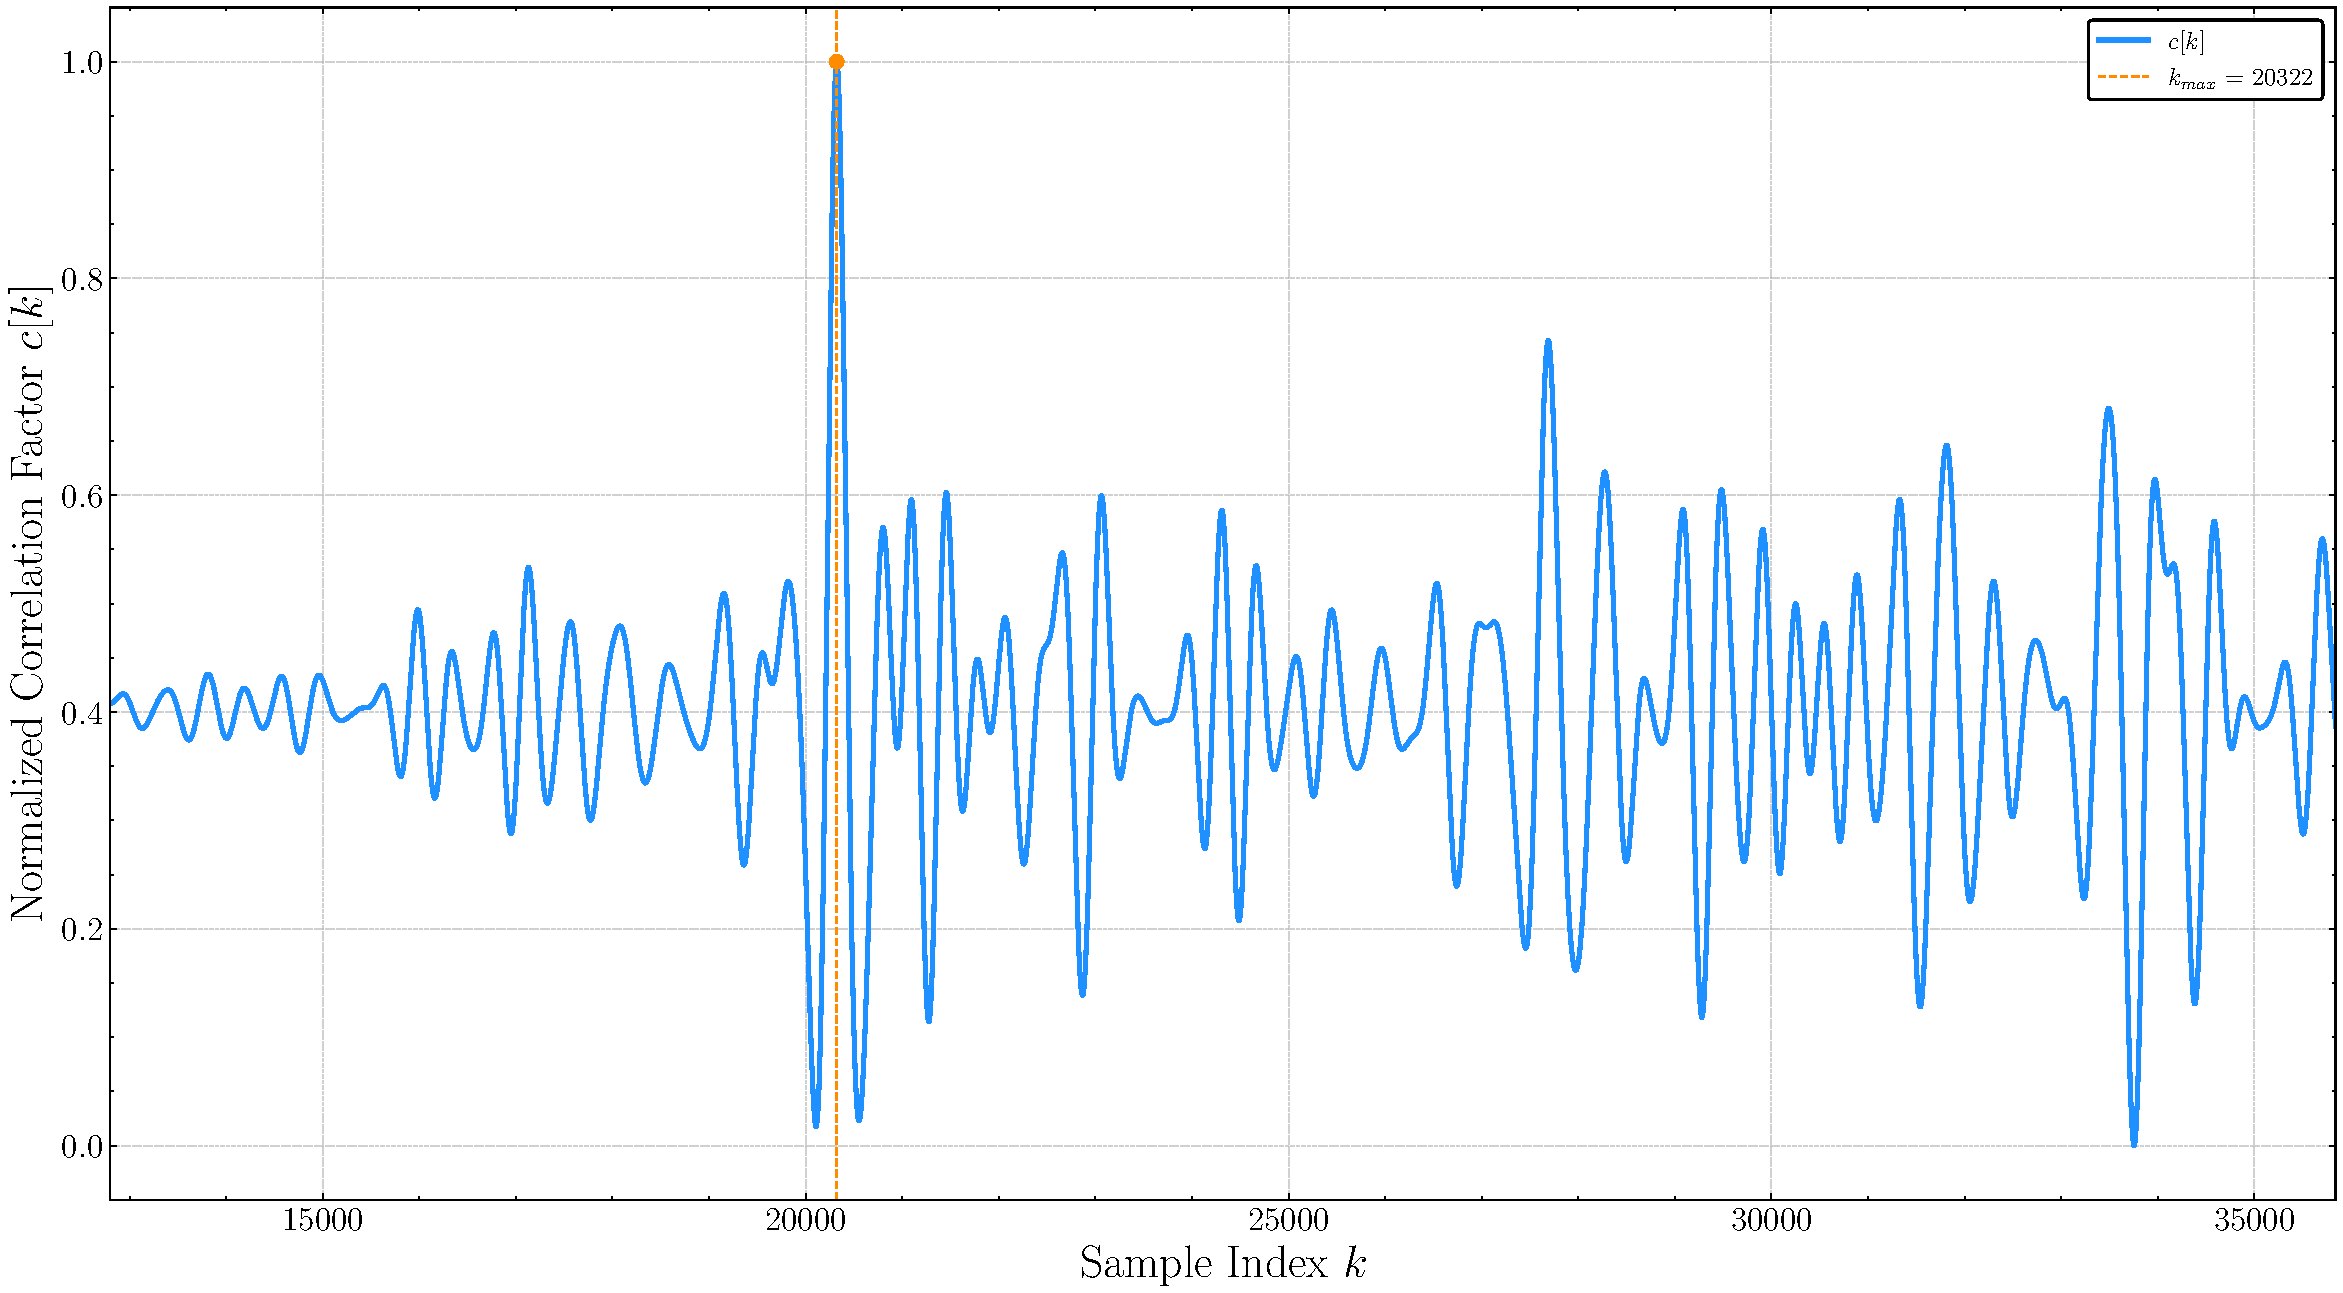
\includegraphics[width=\linewidth]{assets/cap3/receiver_sync_corr.pdf}
\end{figure}

\begin{figure}[H]
	\centering
	\caption{Sicronização de $I$ e $Q$ com vetor de sincronismo}\label{fig:receiver_sync}
	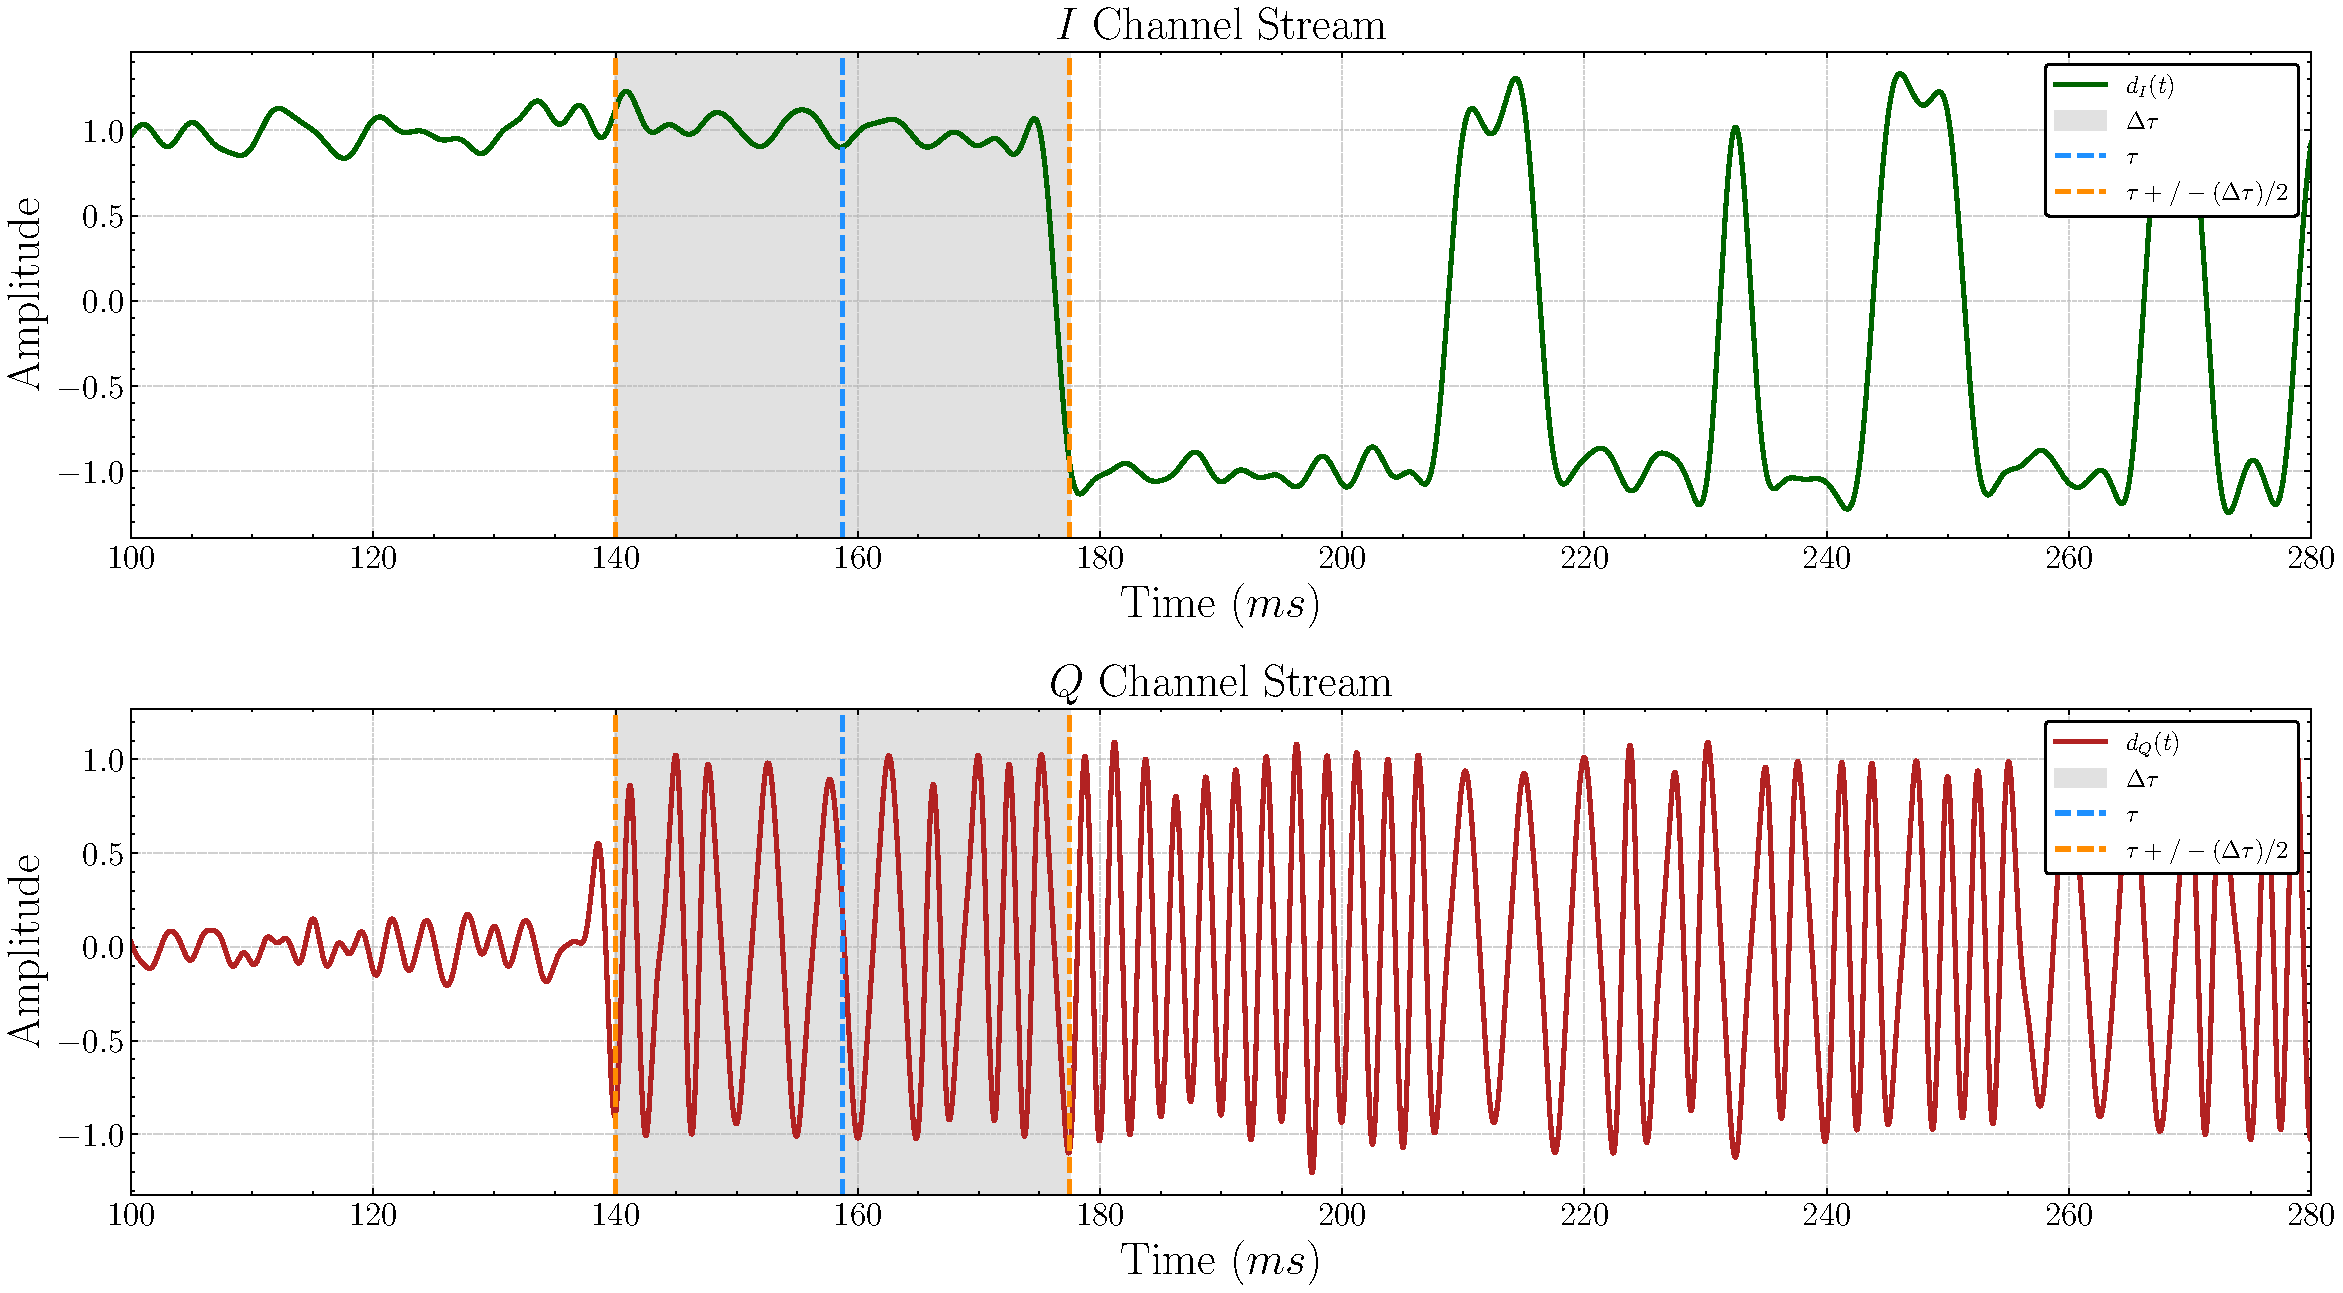
\includegraphics[width=\linewidth]{assets/cap3/receiver_sync_time.pdf}
\end{figure}


\subsection{Decisão de símbolos}\label{sec:decisao_simbolos}

\begin{figure}[H]
	\centering
	\caption{Amostragem dos canais $I$ e $Q$ em $T_b$ a partir de \gls{tau}}\label{fig:receiver_sampler}
	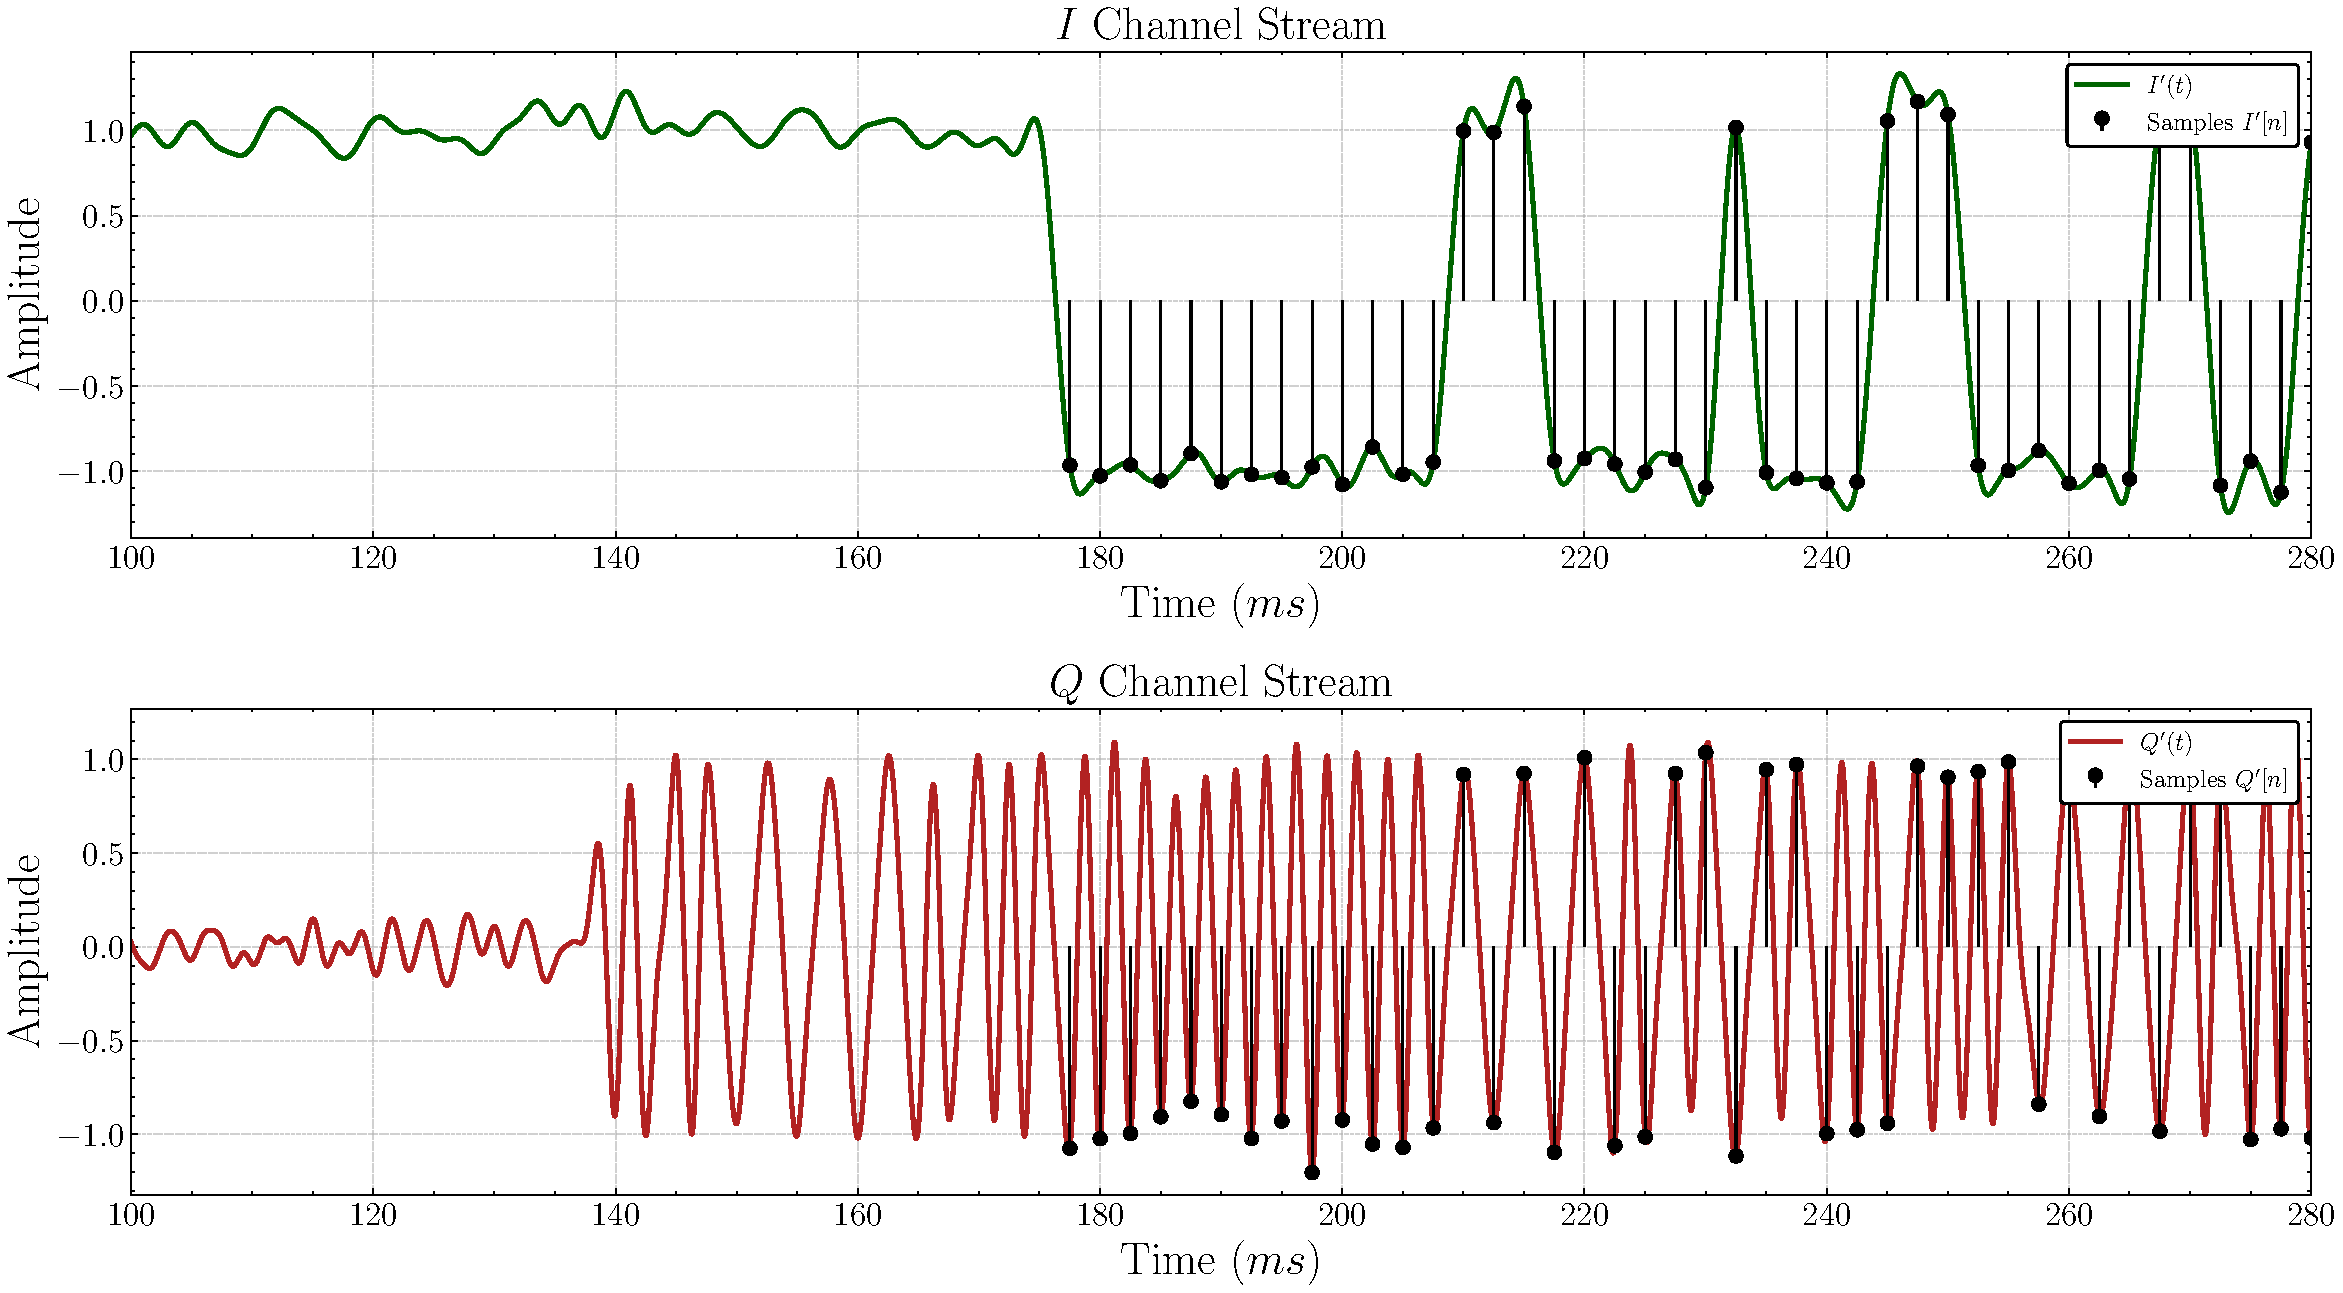
\includegraphics[width=\linewidth]{assets/cap3/receiver_sampler_time.pdf}
\end{figure}

\begin{figure}[H]
	\centering
	\caption{Constelação dos canais $I$ e $Q$ filtrados e amostrados}\label{fig:receiver_const}
	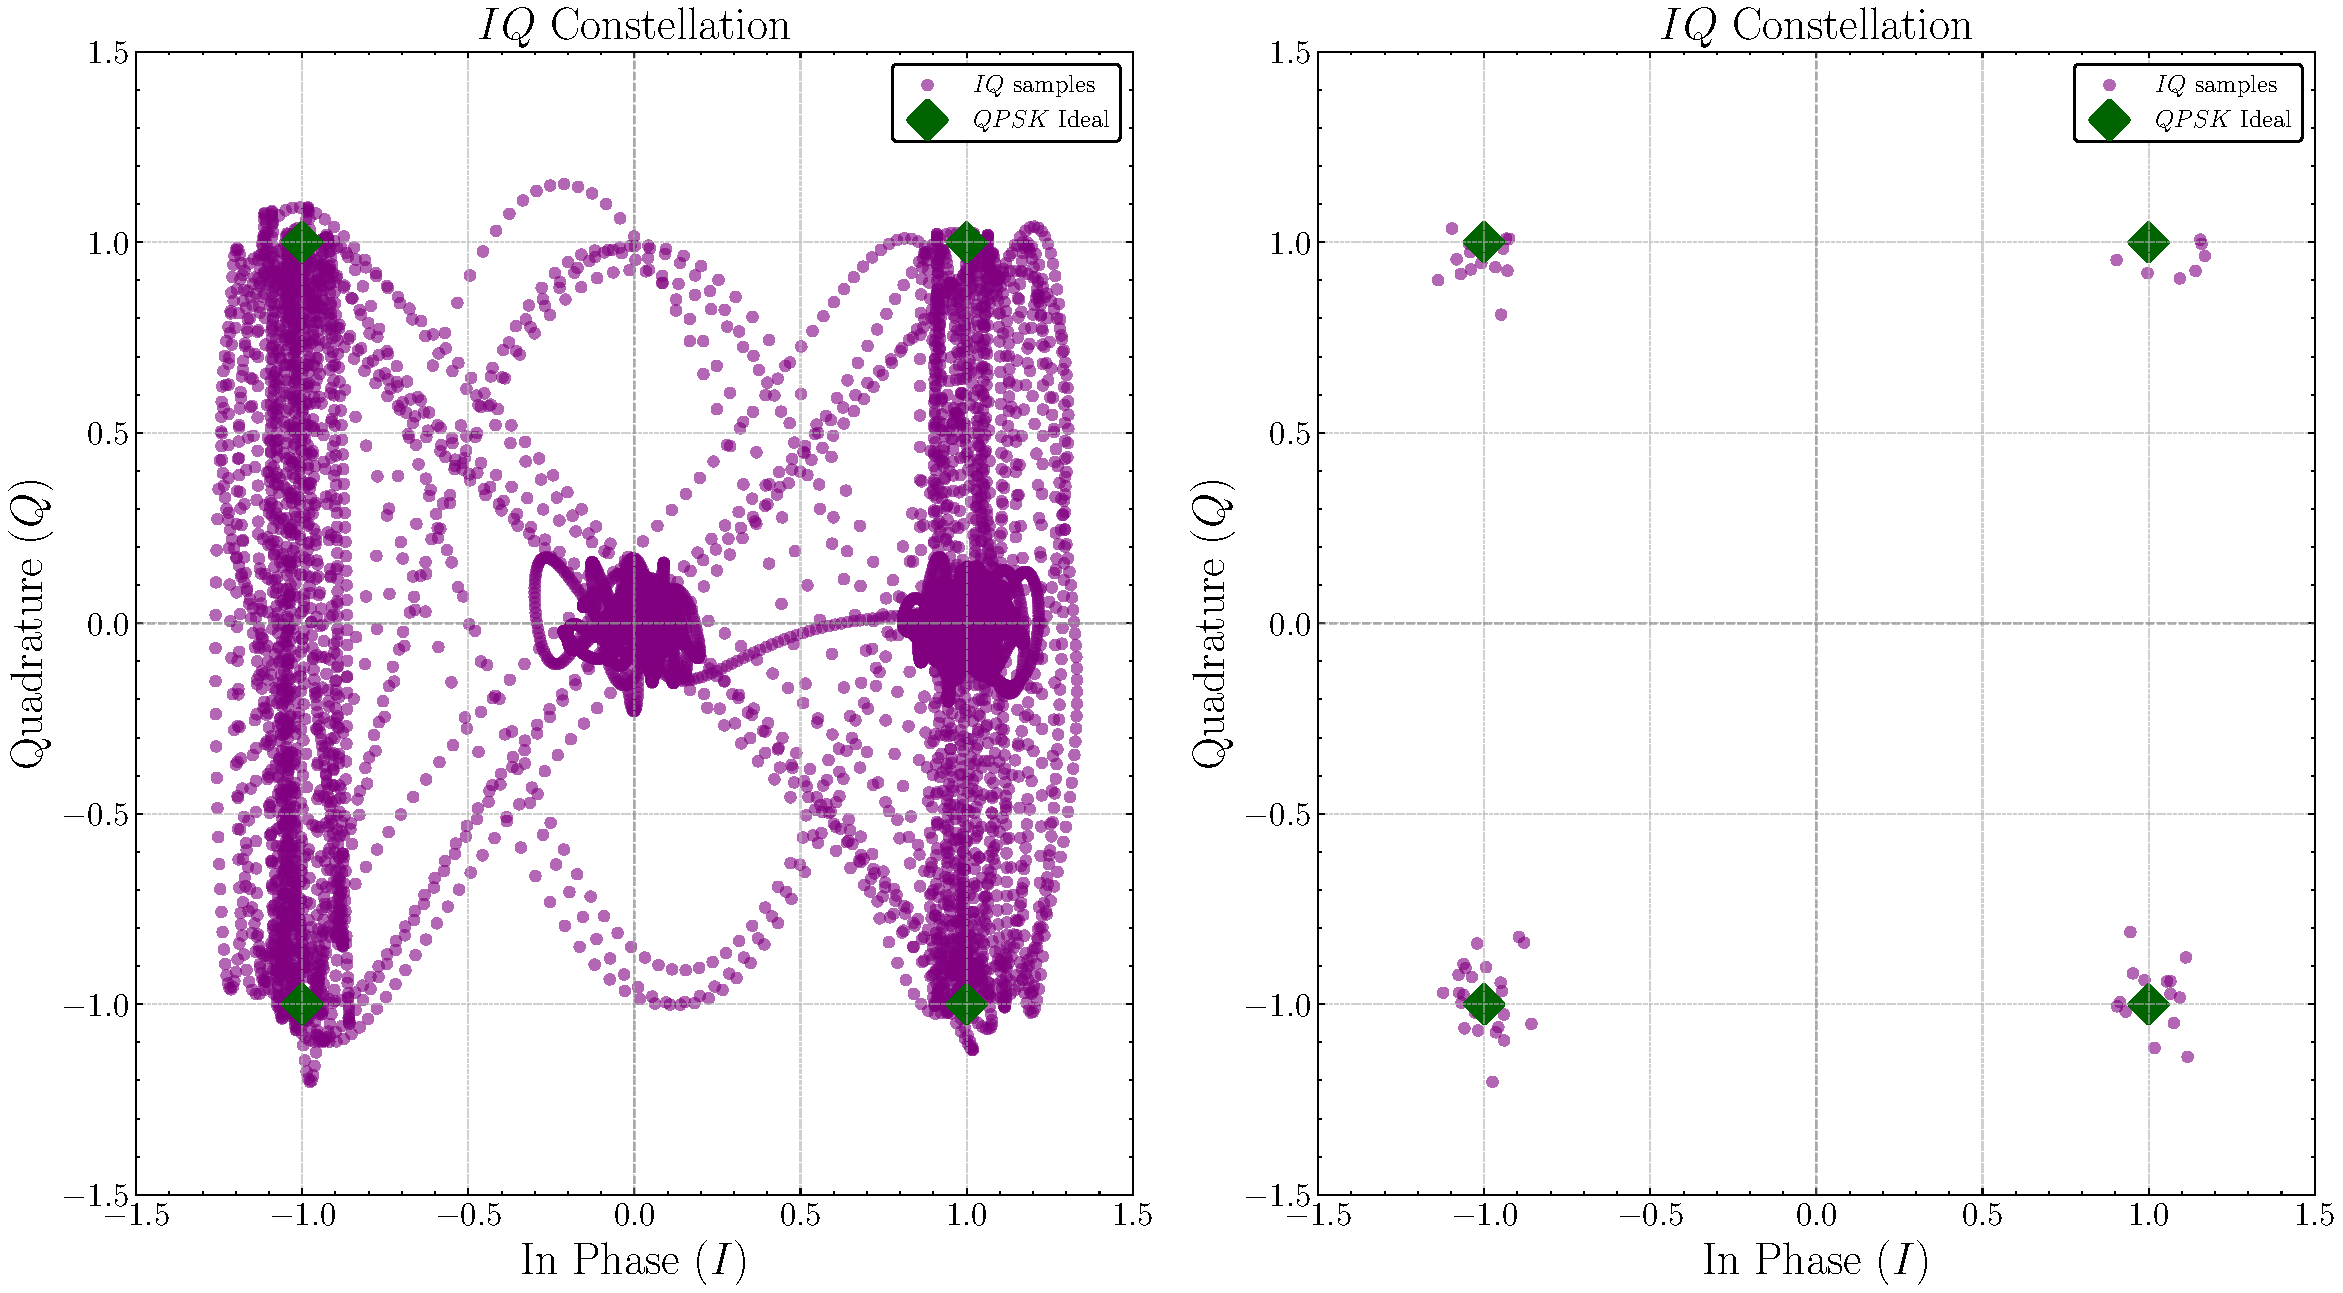
\includegraphics[width=\linewidth]{assets/cap3/receiver_sampler_const.pdf}
\end{figure}

\subsection{Recuperação do Datagrama}\label{sec:decodificacao_convolucional}

\begin{figure}[H]
	\centering
	\caption{Decodificação convolucional dos canais $I$ e $Q$}\label{fig:receiver_conv}
	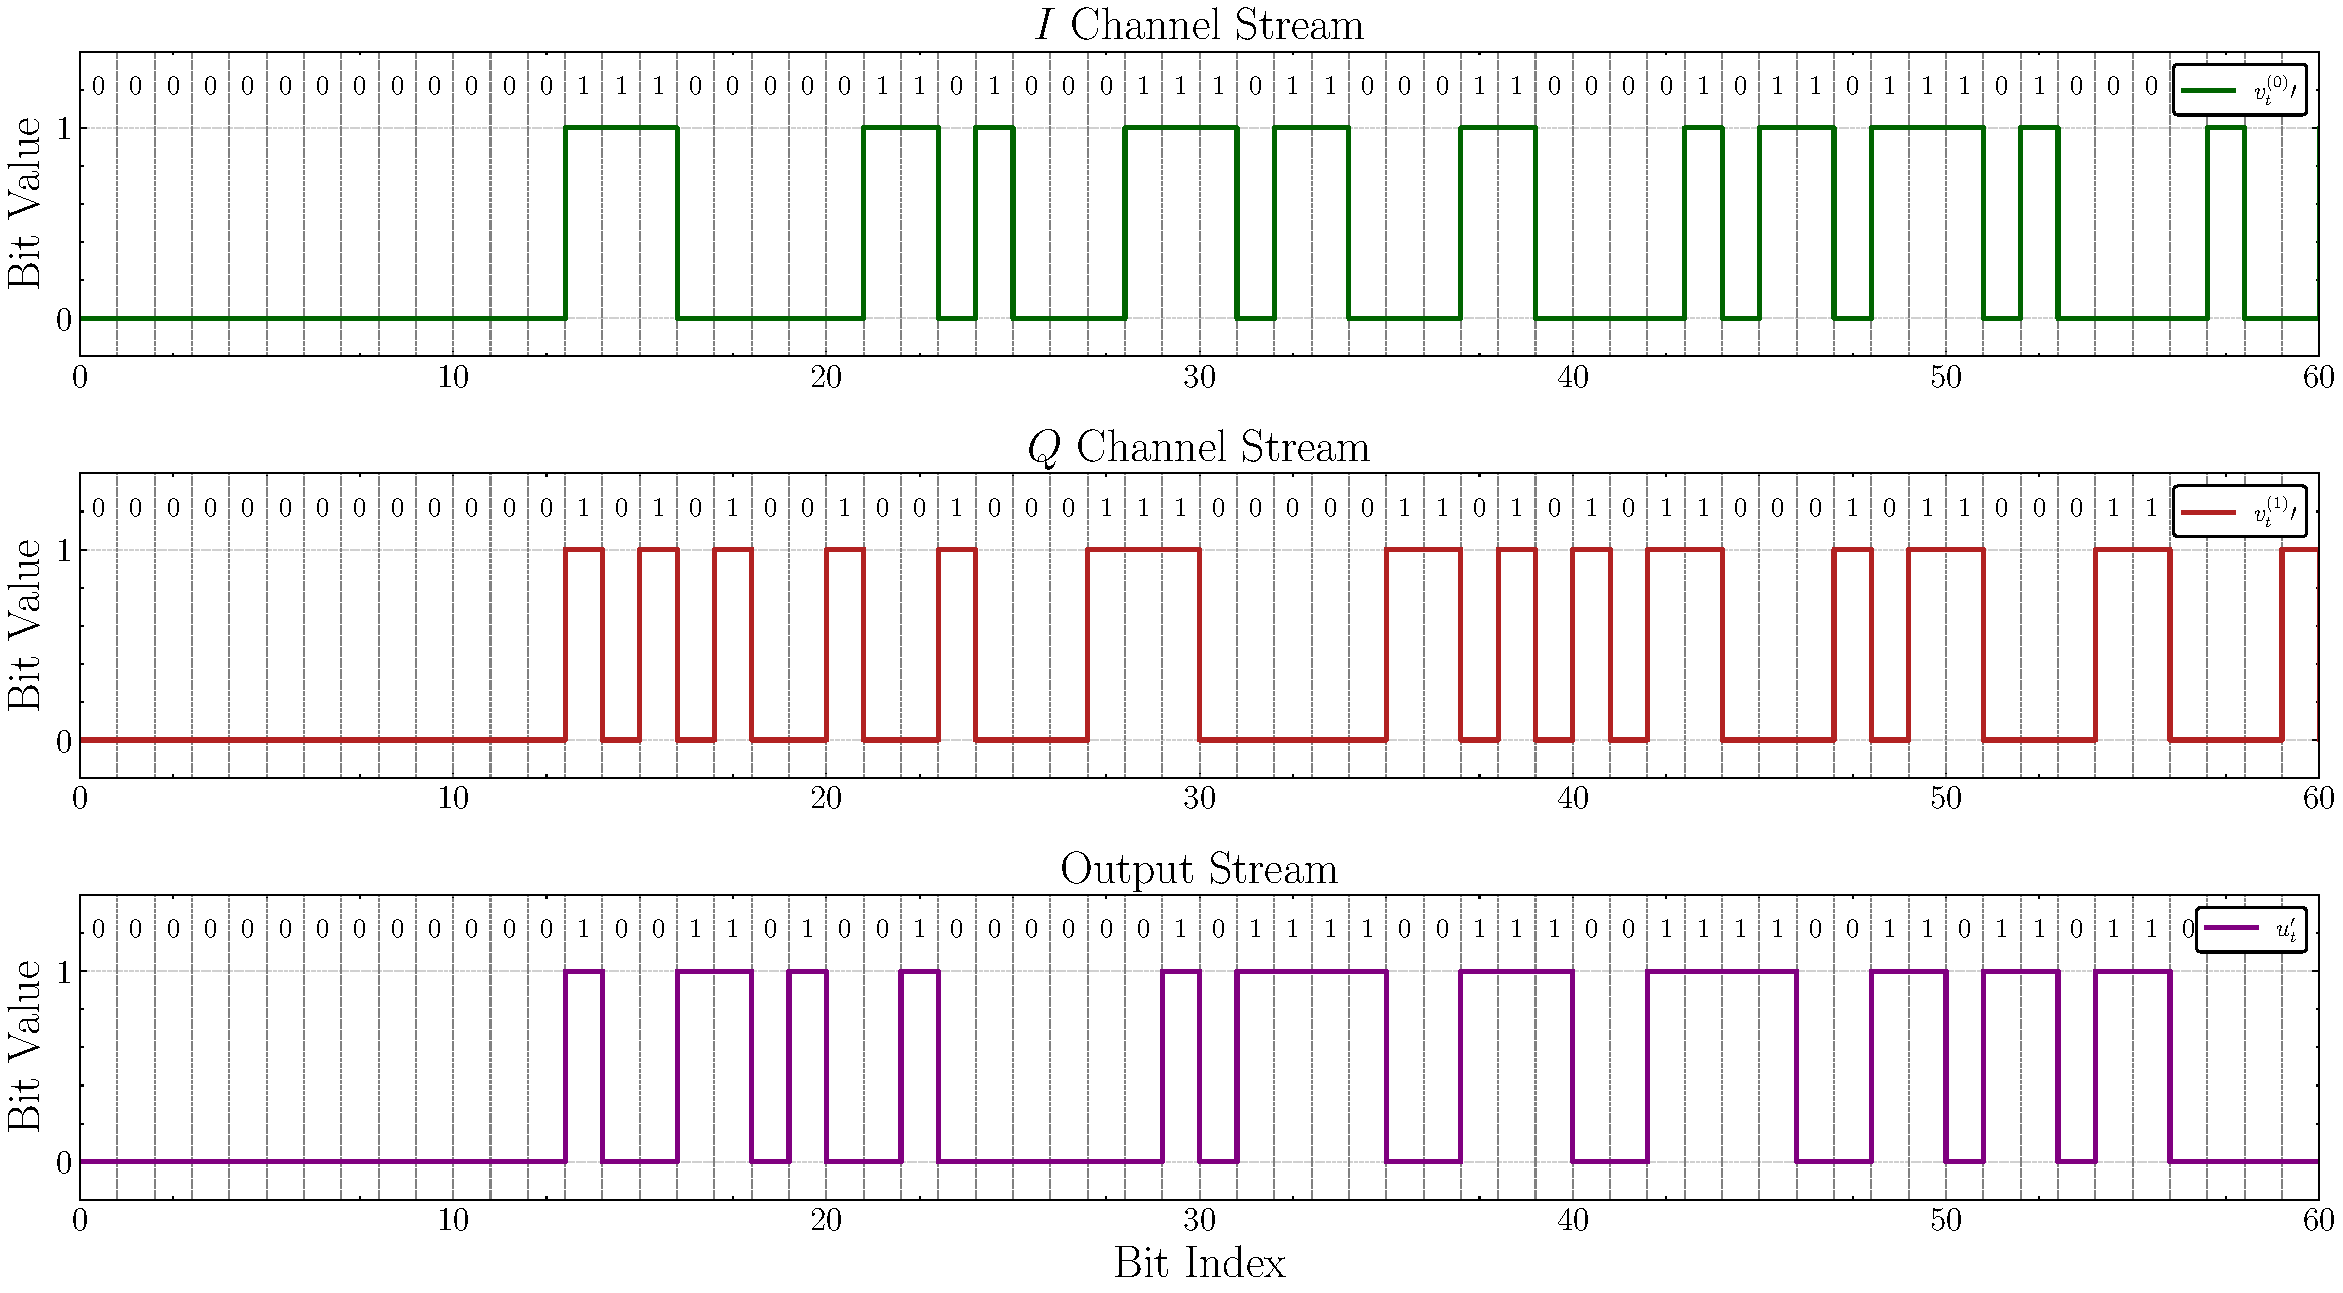
\includegraphics[width=\linewidth]{assets/cap3/receiver_conv_time.pdf}
\end{figure}